\documentclass[a4paper]{report}
\usepackage{color}
\usepackage{listings}
\usepackage{multicol}
\usepackage{hyperref}
\usepackage{mathtools}
\usepackage{url}
\usepackage{pgfplots}
\usepackage{natbib}
\usepackage{xcolor}
\usepackage[english]{babel}
\usepackage[]{algorithm2e}
\usepackage{float}
\usepackage{hyperref}
%\usepackage[utf8]{inputenc}
\usepackage{amsmath}
\usepackage{natbib}
\usepackage{amsfonts}
\usepackage[cc]{titlepic}
\usepackage{graphicx}
\usepackage[colorinlistoftodos]{todonotes}
\usepackage[affil-it]{authblk}
\usepackage{tikz}
%\setlength{\droptitle}{-20em} 
\usetikzlibrary{trees}
\usetikzlibrary{arrows}
\lstset {basicstyle=\tiny,
    language=C++,
    backgroundcolor=\color{blue!7},
    stringstyle=\color{red}}
\title{UPMC Research Intern. at DI ENS Ulm\\ with St\'ephane MALLAT\\Scattering decomposition for massive signal classification :
from theory to fast algorithm and implementation with validation on
international bioacoustic benchmark}
\author{Randall BALESTRIERO\\
\texttt{\url{randallbalestriero@gmail.com}}}

\affil{Pierre et Marie Curie University, Paris 6}
%\author{Vincent LOSTANLEN}
%\affil{Department of Computer Science, ENS Ulm}
%\author{Herv\'e GLOTIN}
%\affil{Aix Marseille Université, ENSAM, Marseille\\
%Universit\'e de Toulon, CNRS, LSIS UMR, La Garde\\
%Institut Universitaire de France (IUF), Paris
%}
%\author{St\'ephane MALLAT}
%\affil{Department of Computer Science, ENS Ulm}

\titlepic{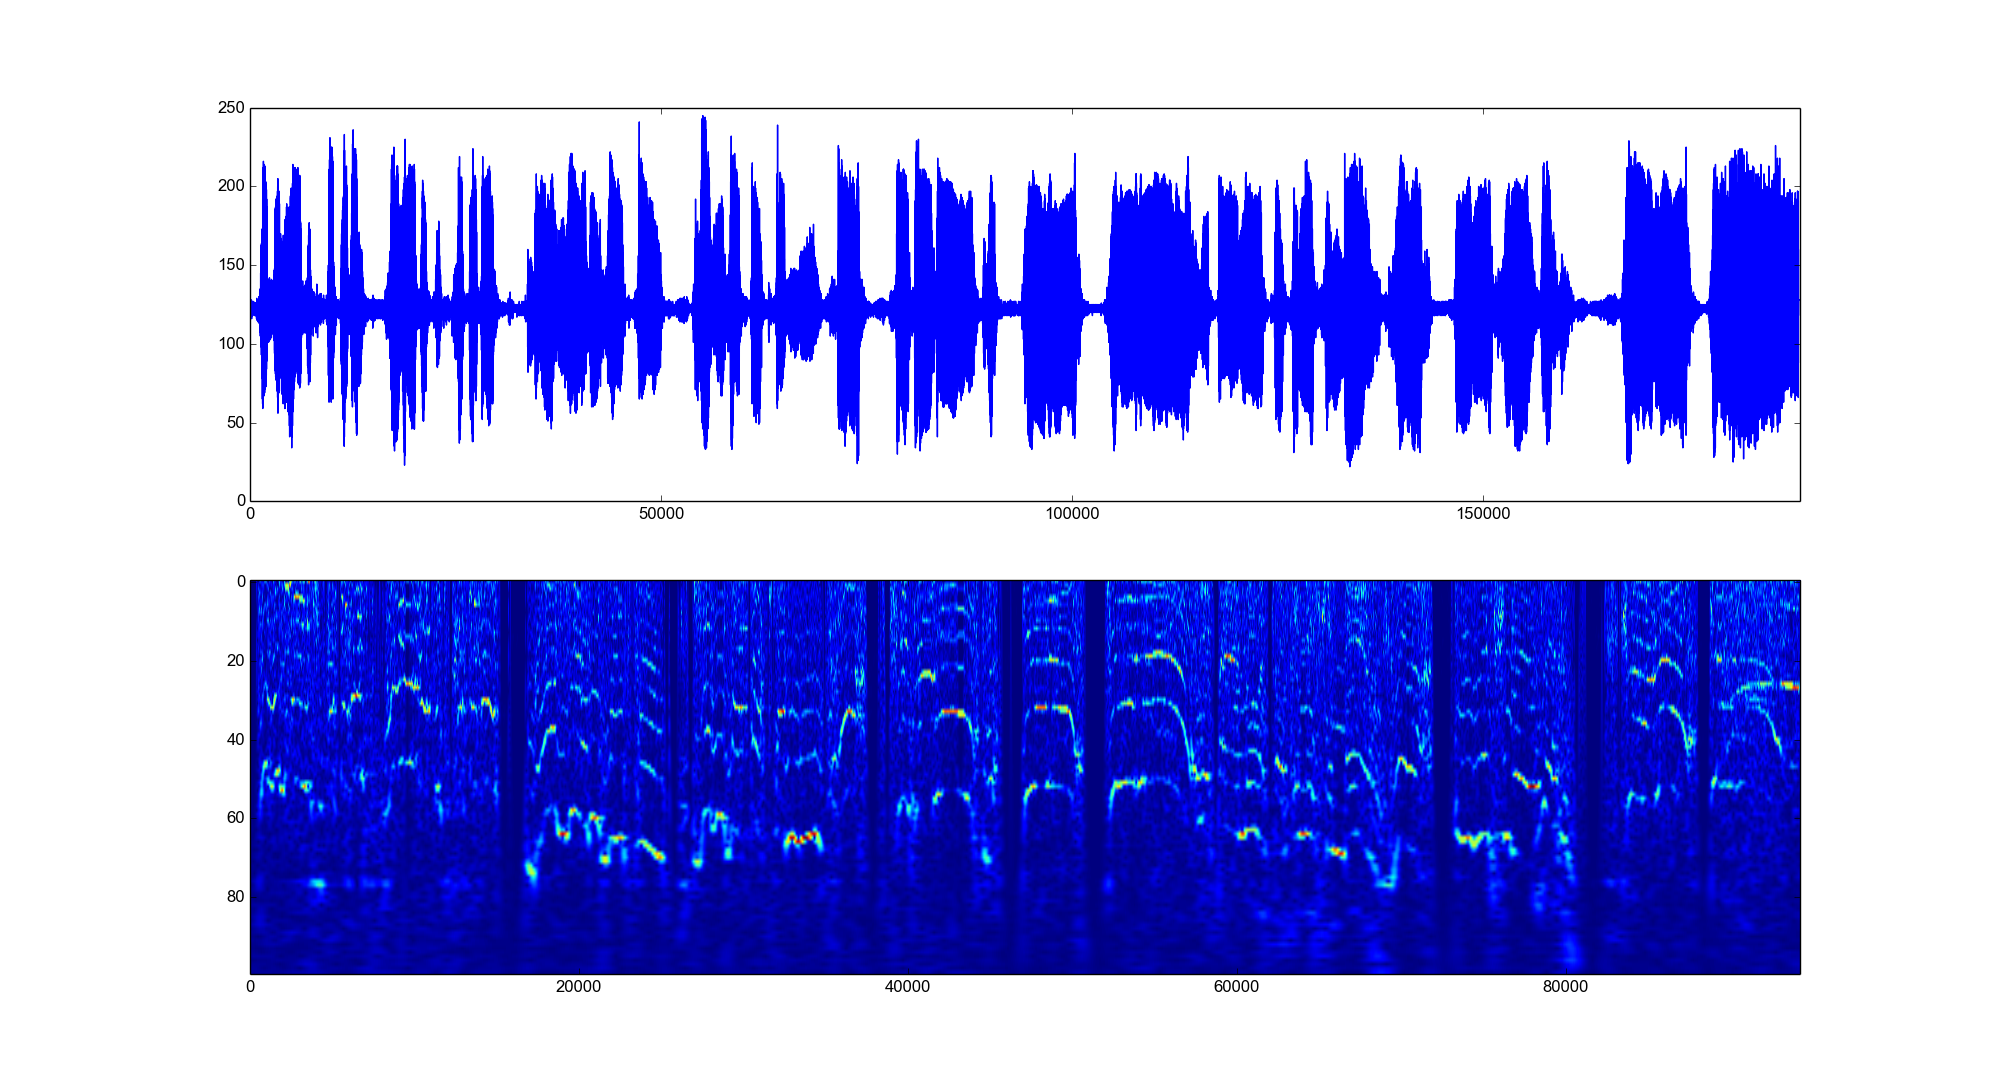
\includegraphics[scale=0.22]{figure_1.png}\\[2pt]

\includegraphics[scale=0.22]{couv_logo.png}}
\date{}



\begin{document}
\maketitle


\newpage

\tableofcontents
\newpage
\section{Introduction}

With the computational power available today, machine learning is becoming a very active field finding its applications in our everyday life. One of its biggest challenge is the classification task involving data representation (the preprocessing part in a machine learning algorithm). In fact, classification of linearly separable data can be easily done. The aim of the preprocessing part is to obtain well represented data by mapping raw data into a "feature space" where simple classifiers can be used efficiently.
For example, almost everything around audio/bioacoustic uses MFCC features until now.
This toolbox gives the basic tools for audio representation using the C++ programming language by providing an implementation of the Scattering Network \cite{m3} which brings a new and powerful solution for these tasks. 
The toolkit of reference in scattering analysis is SCATNET from Mallat et al. \footnote{\url{http://www.di.ens.fr/data/software/scatnet/}}. This
tool is an attempt to have some of the scatnet features more
tractable in large dataset.
Furthermore, the use of this toolbox is not limited to machine learning preprocessing. It can also be used for more advanced biological analysis such as animal communication behaviours analysis or any biological study related to signal analysis.\\
This toolbox gives out of the box executables that can be used by simple bash commands. Finally, for each presented algorithm, a graph is provided in order to summarize how the computation is done in this toolbox.\\

As we will review in the next part, we will need to perform data manipulation on huge dataset. It becomes important to have fast and efficient implementations in order to deal with this new "Big Data" era. The first descriptions concern mandatory utilities, such as audio file IO and basic tools (fft,...) that are necessary for the scattering network implementation.

\part{Fast Scattering}
\chapter{Scattering Network}


The Scattering Network aims to find a better data representation after numerous transformations of a raw input. It's been developed by St\'ephane MALLAT and its team and the only available implementation is in Matlab which provides high-level programming but is not optimal in term of execution time. 
In fact, this algorithm just started to be applied in concrete challenges and finds its limitation in the required time to complete the transformation on massive dataset. We will review its core ideas and the implementation architecture chosen in C++.

\section{Introduction}\label{conv}


The basic idea is to perform series of linear and non linear operations on a $1D$ given input signal $x$. The linear operations are done through the convolutions while the non linear ones are the use of the absolute value on these convolutions. The use of the latter allows fast convergence by the contractive property. The convolutions of the first layer $|x \star \psi_{\lambda_1}|$ are basically decomposing the signal into a wavelet basis. A parallel can be made with the FFT and the complex sine decomposition. In addition, the application of the low-pass filter $\phi$ brings time invariance (of length depending on the $\phi$ support/bandwidth).


The structure itself of the network can be compared to a Convolutionnal Neural Network where the filters are given and fully determined by the meta parameters and not learned during a training phase. This is a huge difference in term of computation time allowing good representation without training. We have to keep in mind that filters generation is also complex and time consuming.


The mapped data into the feature space can be used for simple data analysis or data learning but it finds its best use in classification. In fact, this feature space is much more suited for the use of linear classifier.
Note that in this implementation we won't look at the reconstruction problems since our main goal is not to use the Scattering Network for compression,reconstruction,...
Let's look at the general picture of the scattering network and analyse it briefly.
\\
\begin{figure}[H]
\begin{center}
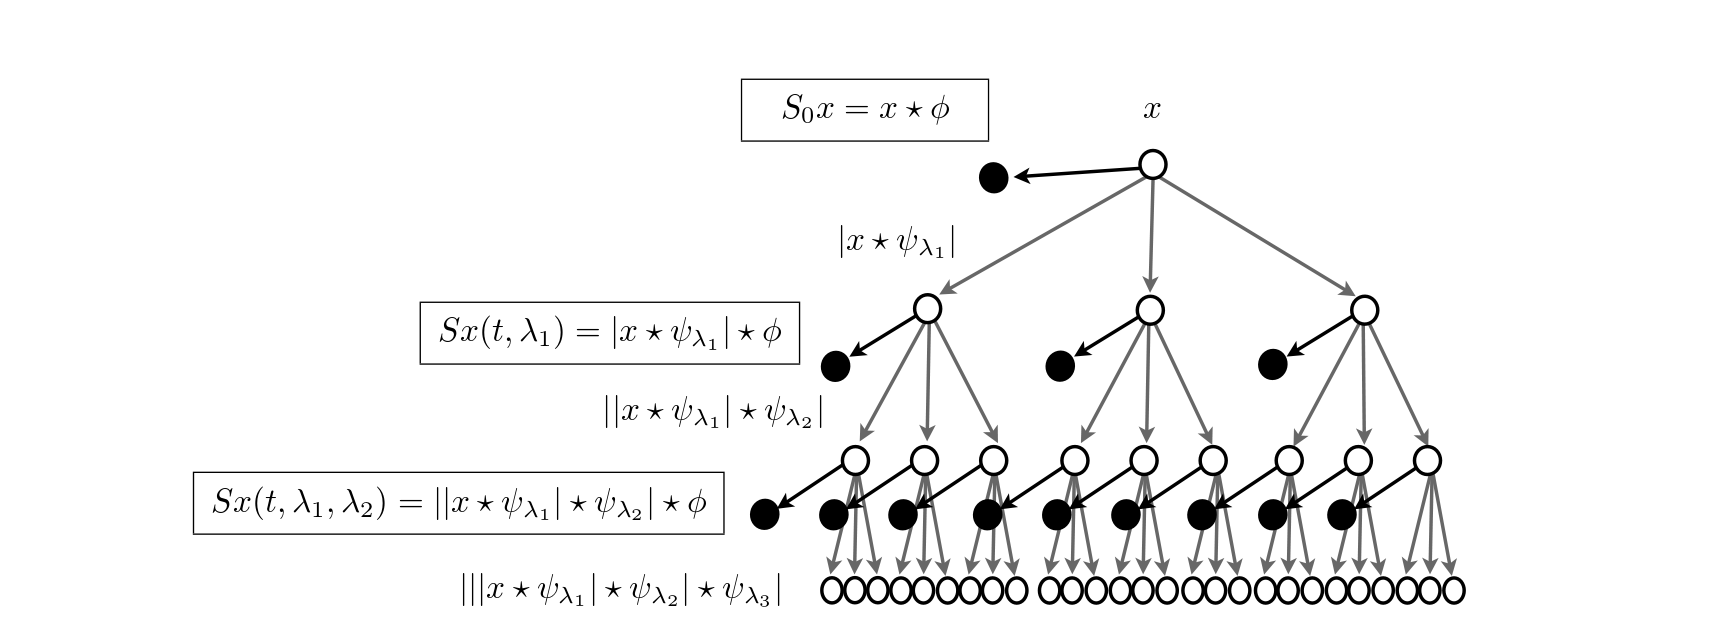
\includegraphics[scale=0.23]{scattering.png}\label{oo}\caption{Scattering Summary.\cite{m2}}
\end{center}
\end{figure}


In this case the scattering network is made of $3$ layers. Each layer has a specific low-pass filter ($\phi_i,i=0,1,2,3$) and high-pass filter banks ($\psi_1,\psi_2,\psi_3$). In our specific case of $1D$ signals, there is only one $\phi$ per layer. Given an input signal $x$ of size $N$ we perform a low-pass decomposition $|x \star \phi_0|:=S_0x$ and a high-decomposition $ x \star \psi_{1,\lambda_1}$. Note that the convolutions are then sub-sampled leading to a output size of $|\lambda_1| \times 2N/T$ for $U_1$. The sub-sampling only reduce coefficient redundancy and depends on the $T$ coefficients. The $i^{th}$ filter of a given high-pass filter bank is generated by the meta parameters of the corresponding layer.
\\Finally on these convolutions is applied the absolute value operation leading to the high-decomposition $U_1:=|x \star \psi_{1,\lambda_1}|$ of the first scattering layer. The scattering coefficients are then easily computed with the application of the low-pass filter $\phi_1$ leading to the scattering coefficient per say $U_1 \star \phi_1:=S_1$. 
\\
Then for the second layer, each one of the previous high-decomposition row is treated as an input signal and the same algorithm is performed again. Details about this will be given in the scattering layer section\ref{ll} but we can already note that the meta parameters are specific to each scattering layer.
Finally let's review what the meta parameters are about :
\begin{itemize}
\item $T$ determines the $\phi$ support/bandwidth, this is basically the invariant time window. Taking a great $T$ leads to huge time invariance but at the cost of variance (and information) loss with respect to the time dimension.
\item $Q$ determines the quality factor (the number of filters per octave)
\item $J$ determines the number of octave to go through.
\item $PE$ (Periodization Extent) is the constant used in the filter periodization ($1$ by default)
\end{itemize}

\section{Filter Bank}
Filters are created given the meta-parameters, the support size an the filter position in the filter bank. Using this, the coefficients $\sigma$ and $\xi$ are deduced.\\
For the $\psi$ generation, it is efficient to loop through $\gamma$ since the meta parameters and the total size of the filters are the same (only the filter number in the filter bank changes). Note that the support of these filters expands when $\lambda$ increases.
On the other hand, creating a specific filter with just the bandwidth and frequency max. position is more efficient and is thus used for the $\phi$ generation. In fact, since only one low-pass filter is made per layer, we just have to compute $\xi$ and $\sigma$ for this filter.


The filters are directly computed in the Fourier domain to speed up the decomposition algorithm, indeed we only have to compute the FFT of the input to perform the decomposition algorithm now. Here $\xi$ corresponds to the central frequency and so to the global maximum position. It can be seen as a position parameter while $\sigma$ is a scale parameter. In practice, in order to generate the filters we always take the mother coefficients that are transformed through a scaling coefficient with exponential rate. We have then as mother coefficients :
\[
\Xi=\frac{\pi}{2}*(2^{-1/Q}+1)
\]
\[
\Sigma=\sqrt{3}*(1-2^{-1/Q})
\]
The scaling factor for the filter $i$ is :$\lambda_i=2^{-i/Q}$ which leads to the following coefficients for any given filter $i$ for a specific layer having the same meta parameters :
\[
\xi_i=\Xi*\lambda_i
\]
\[
\sigma_i=\Sigma*\lambda_i
\]


\paragraph{Filters} In this implementation, high-pass filters are Morlet wavelets while low-pass filters are Gabor filters. Note that Morlet filters are actually another name for Gabor kernels. The difference between the Gabor function (non-zero-mean function) and the Gabor kernel (zero-mean function) is that the Gabor kernel satisfies the admissibility condition for wavelets (integral equals to $0$), thus being suited for multi-resolution analysis. The admissibility condition ensures that the inverse transform and Parseval formula are applicable.

\paragraph{Filter Periodization}
In order to increase resolution of the filters, we can compute them on a bigger interval than the one we are interested in and then periodize them in the Fourier domain :
\[
f(x)=\sum_{n\in \mathcal{Z}} f(x+2\pi n) 
\]
In practice nothing assures the convergence for any function $f$ but our filters are generated through Gaussian functions which actually guarantees the convergence. In practice, we use $n\in \{-PE, -PE+1,...,PE,PE+1 \}$ with $x \in \{ x \in \mathbb{R}, i=0,...,T-1 : x= i*2\pi/T\} $ which is similar to $x \in \{0,2\pi/T,2*2\pi/T,...,(T-1)2\pi/T \} $.
With this definition $x$ covers $[0,2\pi[$ with $T$ points linearly separated by a distance of $1/T$.
In all the examples presented here a periodization extent of $1$ is used.
\\
The $n$ coefficients affect the range on which the wavelet is evaluated which grows with bigger $n$ : 
\[ [  -2\pi * PE, 2\pi*(1+PE)-1/T ] \]
It is then shrunk into the desired support size by the periodization process.

\section{Scattering Layer}\label{ll}
The scattering layer performs the decomposition of the raw input given the meta parameters and the filter banks by performing the decomposition process. 
\\
With the filter bank, all the $\psi$ filters are available and we can apply Littlewood-Paley normalization necessary because of the logarithmic spaced filters.

\paragraph{Decomposition Implementation}
The core of the algorithm lies in this decomposition. Firstly, the convolution defined in the section \ref{conv} is redundant and so is only performed on every $T/2$ spaced points. This implies a reduced output length and faster computation. Thus, it is necessary to perform a periodization before computing the IFFT (allowing a time sub-sampling). The output length must then be $\text{InputSize}*2/T$. Doing this for each $\psi$ filter gives the output of the layer.
Here is a simple scheme to emphasize the algorithm :
\\
\\
\begin{algorithm}[H]
 \KwData{Input,inputN,inputM,Meta Parameters}
 \KwResult{Output,outputN,outputM}
 NumberOfPsis=J*Q\;
 outputN=inputN*NumberOfPsis\;
 outputM=inputM$*2/T$\;
 $\psi$ Filter Bank creation\;
 $\phi$ creation\;
 \For{$i=0 \rightarrow$inputN}{
 inputFFT=FFT(input[i]);))\;
 \For{$j=0 \rightarrow$ NumberOfPsis}{	HighDecomposition[i*NumberOfPsis+j]=abs(IFFT(inputFFT$.*\psi_{L,j}$)\;
 Scattering[i*NumberOfPsis+j]=IFFT(periodize( FFT(HighDecomposition[i*NumberOfPsis+j]$.*\phi_{L}$)))
  }
  }
 \caption{Decomposition Algorithm of the layer $L$}
\end{algorithm}

With "periodize" being the function that will periodize the result in order to sub-sample in the time domain to obtain the desired output size. 
For example the array $[0,1,2,3,4,5]$ is equal to $[3,5,7]$ after a periodization by a factor of $2$.

\chapter{Choice for Fast Audio File Manipulation}

\section{File Structure}
The WAV file is an instance of a Resource Interchange File Format (RIFF) defined by IBM and Microsoft. The header part of this file is made of complementary chunks describing the architecture of the wav allowing easy information storing.
Let's see how these chunks are organized in a WAV file :

\begin{figure}[H]
\begin{center}
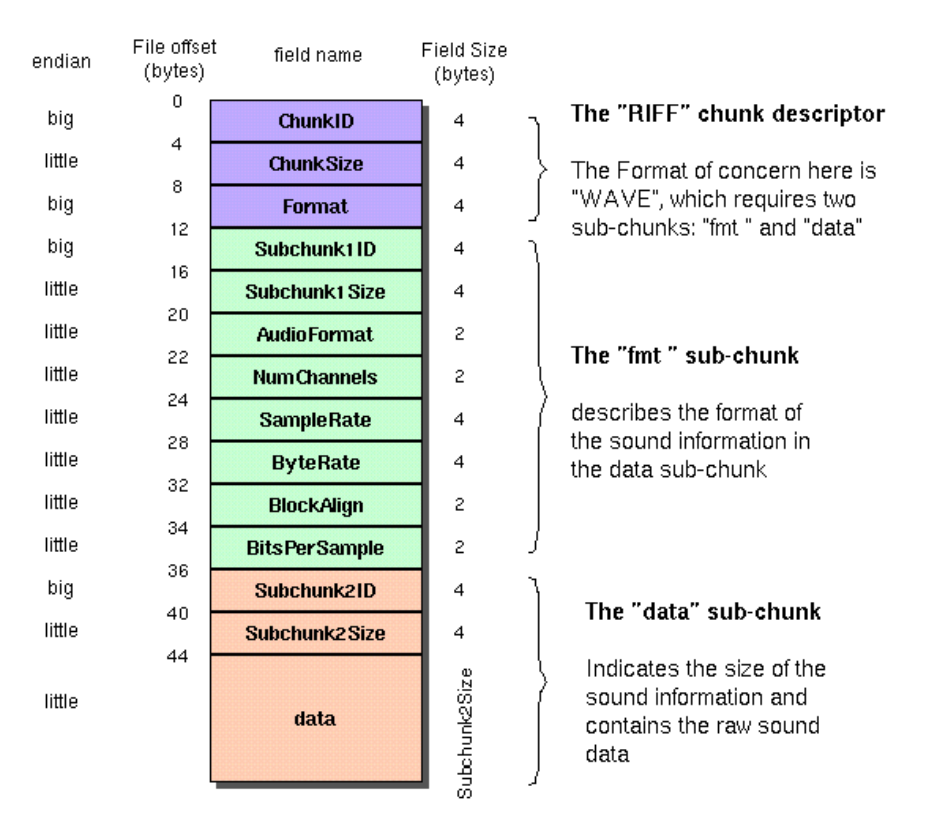
\includegraphics[scale=0.31]{wavformat.png}\caption{The Canonical WAV file format \url{https://ccrma.stanford.edu/
courses/422/projects/WaveFormat/}}
\end{center}
\end{figure}

The file is made of three main chunks each having a specific role that we will describe here.
\subsection*{Chunk}
\begin{itemize}

\item ChunkID identifies the type of the first chunk with four characters : "RIFF".
\item ChunkSize is the size of the file left from this point. It will be 36 (sum of the other chunks sizes) plus Subchunk2Size and this can be easily seen by summing the different sizes on the right of the header representation.
\item Format will be four characters : "WAVE" (this allows us to check if we are really reading a wav file during the process).
\end{itemize}

\subsection*{Sub Chunk 1}
\begin{itemize}
\item SubChunk1ID identifies the second chunk. It is a four characters name : "fmt "  and starts the data description block. 
\item SubChunk1Size is simply the size of this block which is 16. 
\item AudioFormat, also called Format tag, is the option indicating the data compression used. It is almost always equal to $1$ which stands for : no compression is used. 
\item NumChannels is the number of channels ($1$ for mono and $2$ for stereo). 
\item SampleRate is simply the number of samples per second, the frequency. 
\item ByteRate is the average number of bytes per second, this can be found with the following formula : $\text{SampleRate} * \text{NumChannels}*\frac{\text{BitsPerSample}}{8}$. 
\item BlockAlign won't be necessary for us. It can be computed with the formula : $NumChannels*\frac{\text{BitsPerSample}}{8}$.
\item BitsPerSample can either be $8$ or $16$ but in general the later is used.
\end{itemize}

\subsection*{Sub Chunk 2}
\begin{itemize}
\item SubChunk2ID identifies the last chunk block, it is made of the four characters : "data".
\item Subchunk2Size is the size of the file left which is just the size of the data. 
\item Data is the block containing the values of the signal in the standard pulse-code modulation representation.
\end{itemize}


\section{Implementation}
The use of the built-in class WAV is simple, the only thing to provide is the name of the wav file. This can be done during the instantiation of the class or at any other time. Let's look at an example.
\begin{lstlisting}[basicstyle=\tiny]
    WAV<double> Signal("mysignal.wav");
    WAV<double> Signal2;
    "mysignal.wav">>Signal2;
    "mysignal2.wav">>Signal;
\end{lstlisting}
The template parameter can be ignored leading to the default value : float. One instance of the class can be used for different wav files which can be useful. This WAV variable allows easy interactions and can provide informations about the loaded file :

\begin{lstlisting}[basicstyle=\tiny]
    Signal._Size;
    Signal._SampleRate;
    Signal_NumberOfChannel;
    Signal[i];//return the ith value of the loaded signal
\end{lstlisting}
Finally, to export the loaded file two options are available. Firstly, it is possible to export it into a .txt file which only exports the signal data disregarding all the other informations. This loss can be avoided using a special method which exports the data back into a wav file, with the following syntax :

\begin{lstlisting}[basicstyle=\tiny]
    Signal>>"newsignal.txt";//to .txt
    Signal.PrintWav("newsignal.wav");//to .wav
\end{lstlisting}
With this implementation, WAV can be seen as a special type. Note that no normalization is used. In fact, only the user can define the normalizing constant he is interested in (max, $L^2$-norm,...) and so has to apply it after the import.
Finally, for an external use of this toolbox, one should not need to use this class since it is just here as a input/output convenience for the other algorithm we will now describe.

\chapter{Fast Fourier Transform implementation}
\section{Definitions}
A sinusoidal wave is characterised by three parameters: amplitude, frequency and phase.
\begin{itemize}
\item The amplitude is the amount the function varies, positively or negatively, from zero in the y direction.
\item The frequency is how many complete cycles there are of the wave in unit distance on the x axis (which often measures time).
\item The phase is relevant when comparing two waves of the same frequency. It is how much (measured in degrees or radians) one is shifted relative to the other on the x axis.
\end{itemize}
This terminology comes from sound engineering where higher frequency sounds have higher pitch and waves of greater amplitude are louder.
As an alternative of specifying the frequency, the number of cycles in unit distance, we can instead specify the wavelength : the length of one cycle. The higher the frequency, the shorter the wavelength. The lower the frequency the longer the wavelength.
\\
The Nyquist frequency is the maximum frequency that can be detected for a given sampling rate and it is half of this sampling rate. This is because in order to measure a wave one needs at least two sample points to identify it (trough and peak).
We will abbreviate the continuous Fourier transform with CFT and the discrete Fourier transform with DFT.
\paragraph{Interpretation of the CFT}
Using the Euler's formula, we can see the Fourier Transform as a decomposition of a signal into complex sinus by the use of convolutions.
\[
e^{ix}=\cos(x)+i\sin(x)
\]
\begin{align*}
\hat{f}(\xi)&=\int_{-\infty}^{\infty} f(x) e^{-2\pi i x \xi}dx\\
&=\int_{-\infty}^{\infty} f(x) (\cos(-2\pi x \xi)+i\sin(-2\pi x \xi))dx\\
&=\int_{-\infty}^{\infty} f(x) \cos(-2\pi x \xi)+f(x)i\sin(-2\pi x \xi)dx\\
&=\int_{-\infty}^{\infty} f(x) \cos(-2\pi x \xi) dx + \int_{-\infty}^{\infty} f(x)i\sin(-2\pi x \xi)dx
\end{align*}

\section{Fast Fourier Transform}
We will now denote $x_k$ as the $k^{th}$ value on the signal in the time space and $X_k$ the $k^{th}$ value of the signal in the frequency domain, $N$ will denote the length of the signal. A length of $N$ means the indices range from $0$ to $N-1$.
\\
The fast Fourier transform (FFT) is a instance of DFT which is able to perform the DFT in $O(N\log(N))$ complexity.\\
The DFT formula using the Twiddle Factor notation :
\begin{align*}
\forall k \in \mathbb{Z},&X_k=\sum_{n=0}^{N-1} x_n e^{\frac{-2\pi i k n}{N}}\\
&X_k=\sum_{n=0}^{N-1} x_n W_N^{kn}
\end{align*}
As we can see, we need to perform $N$ operations for each $X_k,k\in \{0,1,...,N-1\}$ thus we are in $O(N^2)$ complexity.
\\
Note that it is possible to use the scaling factor :$1/\sqrt{N}$ in order to have an unitary operator (Parseval's theorem) which implies that the sum (or integral) of the square of the function is equal to the sum (or integral) of the square of its transform which is not needed in this toolbox thus not used.\\
In order to go from $N^2$ operations to $N\log(N)$ operations, three main concepts have to be defined :
\begin{itemize}
\item The Danielson-Lanczos Lemma
\item The Twiddle Factor properties
\item The Butterfly Scheme
\end{itemize}

\paragraph{Danielson-Lanczos Lemma}
This theorem is the foundation of the FFT by allowing a divide and conquer strategy. In fact, we have the following relations :
\begin{align*}
X_k=&\sum_{n=0}^{N-1} x_n e^{\frac{-i2 \pi k n}{N}}\\
=&\sum_{n=0}^{\frac{N}{2}-1} x_{2n} e^{\frac{-i2 \pi 2k n}{N}}+ x_{2n+1} e^{\frac{-i2 \pi (2k+1) n}{N}}\\
=&\sum_{n=0}^{\frac{N}{2}-1} x_{2n} e^{\frac{-i2 \pi k n}{N/2}}+\sum_{n=0}^{\frac{N}{2}-1}x_{2n+1} e^{\frac{-i2 \pi 2k n-i2 \pi n}{N}}\\
=&\sum_{n=0}^{\frac{N}{2}-1}x_{2n} e^{\frac{-i2\pi k n}{N/2}}+W_N^k\sum_{n=0}^{\frac{N}{2}-1}x_{2n+1} e^{\frac{-i 2 \pi k n}{N/2}}
\end{align*}
For every $X_i$ we can now divide the $N$ sums into two different summation group (Even and Odd). Note that for the special case $N=2$ the sums are removed and n is replaced by $0$ which means that we are left with a simple linear combination of the input signal and the Twiddle Factor. 
If we apply this recursively we obtain the following architecture :


And now for any given input size we are able to break it done into a linear combination of the input signal with twiddle factors.
For example, if $N=4$ we have after full decomposition :
\[
X_k=x_0+W_2^kx_2+W_4^kx_2+W_4^kW_2^kx_3
\]
And for $N=8$ :
\[
X_k=x_0+W_2^kx_4+W^k_4x_2+W_4^kW_2^kx_6+W_8^kx_1+
W_8^kW_2^kx_5+W_8^kW_4^kx_3+W_8^kW_4^kW^k_2x_7
\]
This puts a constraint though, the signal length has to be a power of $2$. The number of decomposition is thus $\log_2 (N)$.
If the signal size is not a power of $2$ it is necessary to use zero padding (add as may $0$ as necessary at the end of the input). Padding with $0$ in time domain leads to an interpolation of the FFT. Middle zero padding the FFT (in the frequency domain) interpolates the IFFT (time domain). Periodizing in the frequency domain implies sub-sampling in the time domain (this will be useful for the Scattering Network).
\\
One last thing to notice here is the order of the input values in the decomposition. Because of the nature of this decomposition (even/odd) we end up with the $x$ terms being rearranged in a specific order : the bit-reversal order. This can be found by taking the symmetric of the binary position of the input value as seen in this little example for $N=8$:
\begin{align*}
0:000\rightarrow000:0\\
1:001\rightarrow100:4\\
2:010\rightarrow010:2\\
3:011\rightarrow110:6\\
4:100\rightarrow001:1\\
5:101\rightarrow101:5\\
6:110\rightarrow011:3\\
7:111\rightarrow111:7\\
\end{align*}

\paragraph{Twiddle Factor Properties}
Complexity has already been broken down but we can still optimize the implementation by exploiting the Twiddle Factor properties using roots of unity properties. In fact we have :
\[
W_N^k=e^{\frac{-i 2 \pi k}{N}}=\cos(2\pi k/N)-i\sin(2 \pi k/N)
\]
Thus for $N=2$:
\begin{align*}
&W^0_2=W^2_2=W_2^4=...\\
&W_2^1=W_2^3=W_2^5=...
\end{align*}
\\And for $N=4$
\begin{align*}
&W_4^0=W_4^4=W_4^8=...\\
&W_4^1=W_4^5=W_4^9=...\\
&W_4^2=W_4^6=W_4^{10}=...\\
&W_4^3=W_4^7=W_4^{11}=...
\end{align*}
And so on using trigonometric properties, with functions here being $N\pi$-periodic.
So using this will allow us to perform less Twiddle Factor computation at each level.
\paragraph{Butterfly Scheme}
Finally, the last brick is the butterfly scheme that can be seen in the next diagram\ref{bb} allowing an in-place FFT which is memory friendly.

\section{Inverse Fourier Transform}
In order to simplify the algorithm we sill use the following formula :
\[
IFFT(x)=\frac{1}{N}conj(FFT(conj(x)))
\]
\section{Algorithm}
Firstly, our implementation is made of three nested loops, the main one which will go through the $\log(N)$ levels of decomposition. The second one will go through the blocks inside a specific level (the last level as $1$ block whereas the first level as $N/2$ blocks). Finally the last loop will go inside a block (a block on the first decomposition level will have size $2$ while the block in the last decomposition level will be of size $N$). For each level ($i$), only $2^i$ Twiddle factors are computed in the main loop where $i$ is the decomposition level from $0$ to $\log(N)-1$. A simple temporary variable is used in order to perform the swapping operations. Here is an instance of this implementation for $N=8$ and a human friendly output explaining the performed steps.
\begin{figure}[H]
\begin{center}
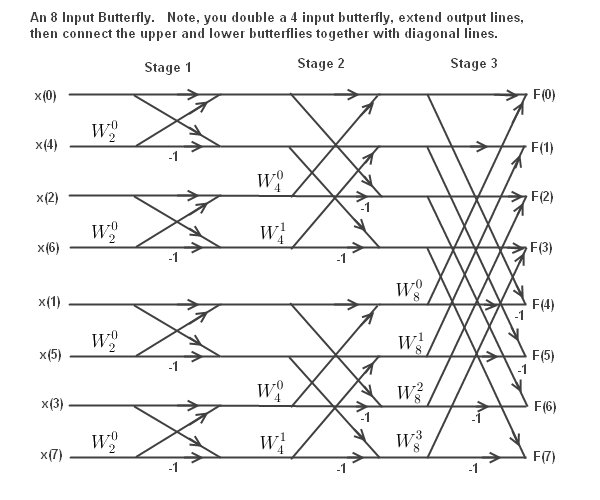
\includegraphics[scale=0.7]{Butterfly8.jpg}\label{bb}
\caption{Full FFT computation with $N=8$ \cite{learnfft}}
\end{center}
\end{figure}
This simple example performs the following computation in the implemented algorithm :

\begin{lstlisting}[basicstyle=\tiny,caption=Computation done during the FFT computation of a signal of size $8$. Each column represents the overall loop 9$log(N)$ iterations. $W$ is the Twiddle Factor and each block is the inner loop performing the butterfly scheme.]

Level : 0
   W[0]=W(0,2)
   Block : 0
     signal[1]*=W[0]
     tmp=signal[0]
     signal[0]+=signal[1]
     signal[1]=tmp-signal[1]

   Block :  1
     signal[3]*=W[0]
     tmp=signal[2]
     signal[2]+=signal[3]
     signal[3]=tmp-signal[3]

   Block :  2
     signal[5]*=W[0]
     tmp=signal[4]
     signal[4]+=signal[5]
     signal[5]=tmp-signal[5]

   Block :  3
     signal[7]*=W[0]
     tmp=signal[6]
     signal[6]+=signal[7]
     signal[7]=tmp-signal[7]
Level :  1
   W[0]=W(0,4),W[1]=W(1,4)
   Block :  0
     signal[2]*=W[0]
     tmp=signal[0]
     signal[0]+=signal[2]
     signal[2]=tmp-signal[2]
     signal[3]*=W[1]
     tmp=signal[1]
     signal[1]+=signal[3]
     signal[3]=tmp-signal[3]

   Block :  1
     signal[6]*=W[0]
     tmp=signal[4]
     signal[4]+=signal[6]
     signal[6]=tmp-signal[6]
     signal[7]*=W[1]
     tmp=signal[5]
     signal[5]+=signal[7]
     signal[7]=tmp-signal[7]
Level :  2
   W[0]=W(0,8),W[1]=W(1,8)
   W[2]=W(2,8),W[3]=W(3,8)
   Block :  0
     signal[4]*=W[0]
     tmp=signal[ 0 ]
     signal[0]+=signal[4]
     signal[4]=tmp-signal[4]
     signal[5]*=W[1]
     tmp=signal[1]
     signal[1]+=signal[5]
     signal[5]=tmp-signal[5]
     signal[6]*=W[2]
     tmp=signal[2]
     signal[2]+=signal[6]
     signal[6]=tmp-signal[6]
     signal[7]*=W[3]
     tmp=signal[3]
     signal[3]+=signal[7]
     signal[7]=tmp-signal[7]
\end{lstlisting}

The Twiddle Factors are computed at the start of each main loop computing the needed values which are then reused throughout the blocks, meaning that for the first level only one value is computed and then reused all along the blocks.
Here is an example of the use :

\begin{lstlisting}[basicstyle=\tiny]
    WAV<> wav("signal.wav");//load a wav into float type array
    fft<> signalfft(signal.ptr(),signal._Size);//default padding option=1
    signalfft.ComputeFFT();
    signalfft.ComputeIFFT();//get back to the original signal
    signalfft[2];//access the second coefficient
    signalfft>>"signalfft.txt";//export it
    wav<<"processed.wav";//load a new wav
    signalfft.ComputeFFT(wav.ptr(),wav._Size);//perform a new FFT
\end{lstlisting}
Note that the parameters of the fft class are by default float and float, the first one stands for the type of the input signal and the latter for the coefficients type (complex$<$float$>$). Finally the padding option which by default is $1$ can be set to $0$ if the user is sure that the given signal is already a power of $2$, this force to skip the padding part resulting in faster computation. Also the coefficients are stored as complex type even after having performed an IFFT meaning that one needs to use a typecast to retrieve the original float type signal for example.


\section{Graph}
\begin{figure}[H]
\begin{center}
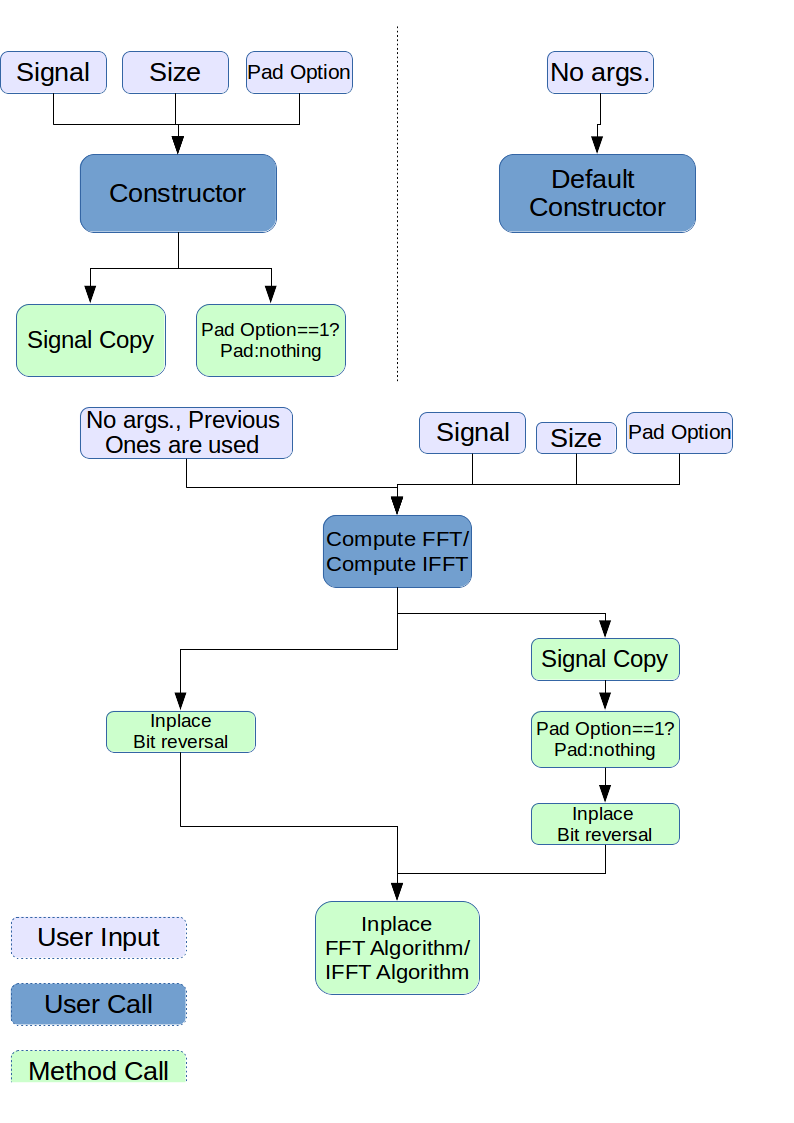
\includegraphics[scale=0.31]{fft_diagram.png}\caption{FFT Summary Diagram}
\end{center}
\end{figure}

\chapter{Spectrogram}
Each $X_k$ is a complex number that encodes how strongly the oscillation at this frequency is represented in the data but by doing an FFT we loose the time component. A useful tool is the spectrogram allowing to retrieve part of the time information. The main idea is to perform multiples FFT on a signal each one being located enough in time so the frequency information gained by the FFT can also be linked to a more or less specific time position in the signal. Note however that precision in both time and frequency is impossible to get but depending on the needs one can choose which one to enhance by modifying the size of the considered window. Larger window gives better frequency resolution but lesser time precision and vice-versa. It is easy to picture the fact that smaller windows are better for the high frequency part allowing good time precision while for low frequency a larger window has to be used for being able to capture it. This problem is lessen in wavelet decomposition and thus the scattering network since this window size is not constant any more.
\section{Algorithm}
Conceptually a spectrogram is computed with the following scheme : 
\begin{itemize}
\item splitting the signal into overlapping (or not) parts of equal length defined by the user.
\item applying to each of these chunk a windowing function (typically hanning or hamming) in order to remove artefacts by periodizing the function so the limit points (start and end of the chunk) are equal. This part is called apodization
\item computing the FFT on each of these chunks
\item for each computed FFT, taking the absolute value of the coefficients will give the columns of the spectrogram.

\end{itemize}
The windowing is needed since the FFT computation presumes that the input data repeats over and over. This is important when the initial and final values of the data are not the same because the discontinuity causes artefacts in the spectrum computed by the FFT.
\\
In addition, in this toolbox, only the first half of the FFT coefficient are put into the spectrogram thus avoiding symmetrical redundancy. This is due to the fact that our input signal is real and so the second half of the FFT coefficients is simply the complex conjugate of the first half, since in the spectrogram we display the absolute value of the coefficients, we get symmetry about the middle point.
\\ 
Most window functions afford more influence to the data at the center of the window than to the data at the edges, which represents a loss of information. To mitigate that loss, it is common to use overlapping in time (usually $50\%$).
\section{Implementation}
It is important to note that the spectrogram ($2D$-matrix) is stored by column and not by line for faster computation. In fact, during the spectrogram calculation we need to access this matrix column-wise. The operator [] returns the column while the operator () takes two arguments and return the corresponding value in a normal way. Let's look at an example :

\begin{lstlisting}[basicstyle=\tiny]
    spectrogram<> b("signal1.wav",256,0.25);//default window function : hamming
    WAV<> wav("signal2.wav");//load another wav
    b.Perform(wav.ptr(),wav._Size);//compute spectrogram given these new entries
        //and default parameters with the already declared spectrogram variable
    b>>"lifespectro.txt";//write the matrix into a txt file
    b[1][0];//second column,first element
    b(0,1);//first line second element same result as above
\end{lstlisting}

The template parameter defines the coefficients type. The default value is float. Also note that no transformation is performed after the absolute value is computed, which means that if one want to apply a logarithmic function (most common one) this has to be done after computation. 
\\
The apodization can be done using one of the available windowing function : 
\begin{itemize}
\item Hamming
\item Hanning
\item triangular
\item Hann Poisson
\end{itemize}
but can also be used with a specific user defined function passed as last argument when calling the Perfom method.
\section{Graph}
The spectrogram graph is simple and emphasizes the default parameters of the class/methods.
\begin{figure}[H]
\begin{center}
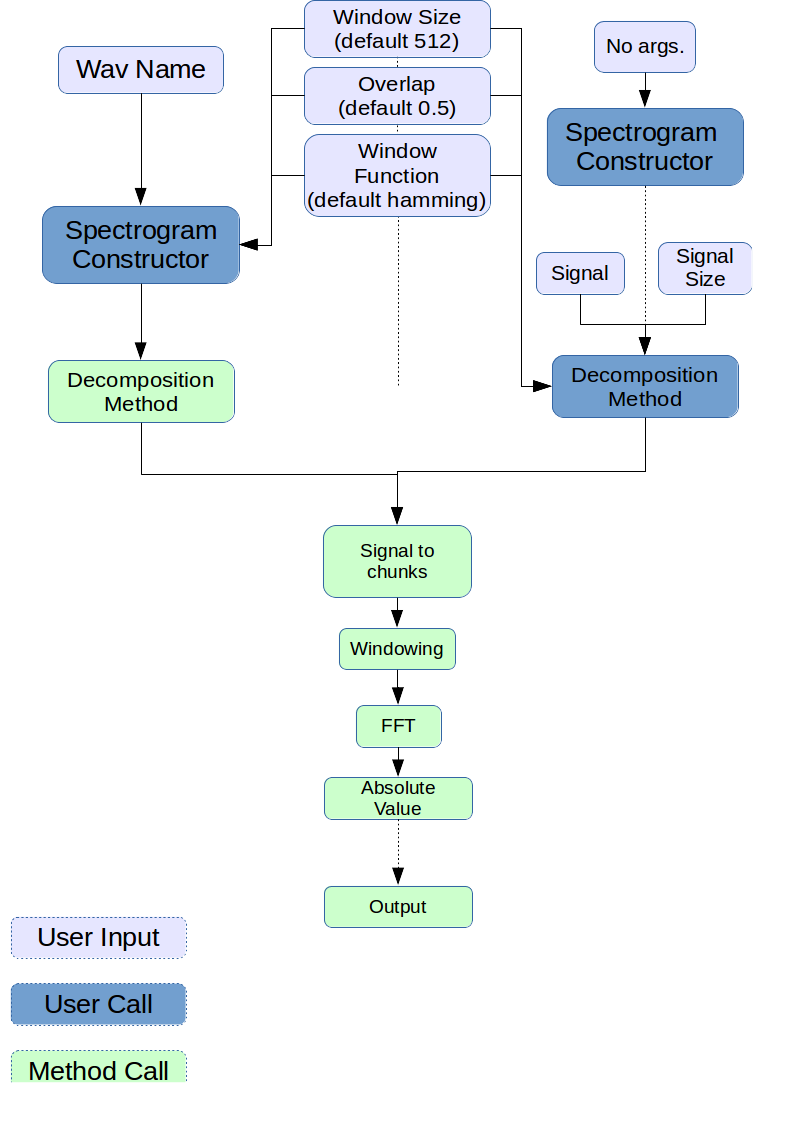
\includegraphics[scale=0.31]{spectro_diagram.png}\caption{Spectrogram Summary Diagram}
\end{center}
\end{figure}
\section{Examples}
Let's look at some spectrogram examples. Note that a logarithmic function has been applied to the computed values (improving coefficient representation for us).
The signals are from a bird of the BIRDLIFE CLEF Challenge 2014 \footnote{\url{http://www.imageclef.org/lifeclef/2015}}.
 and a Inia dolphin.
\begin{figure}[H]
\begin{center}
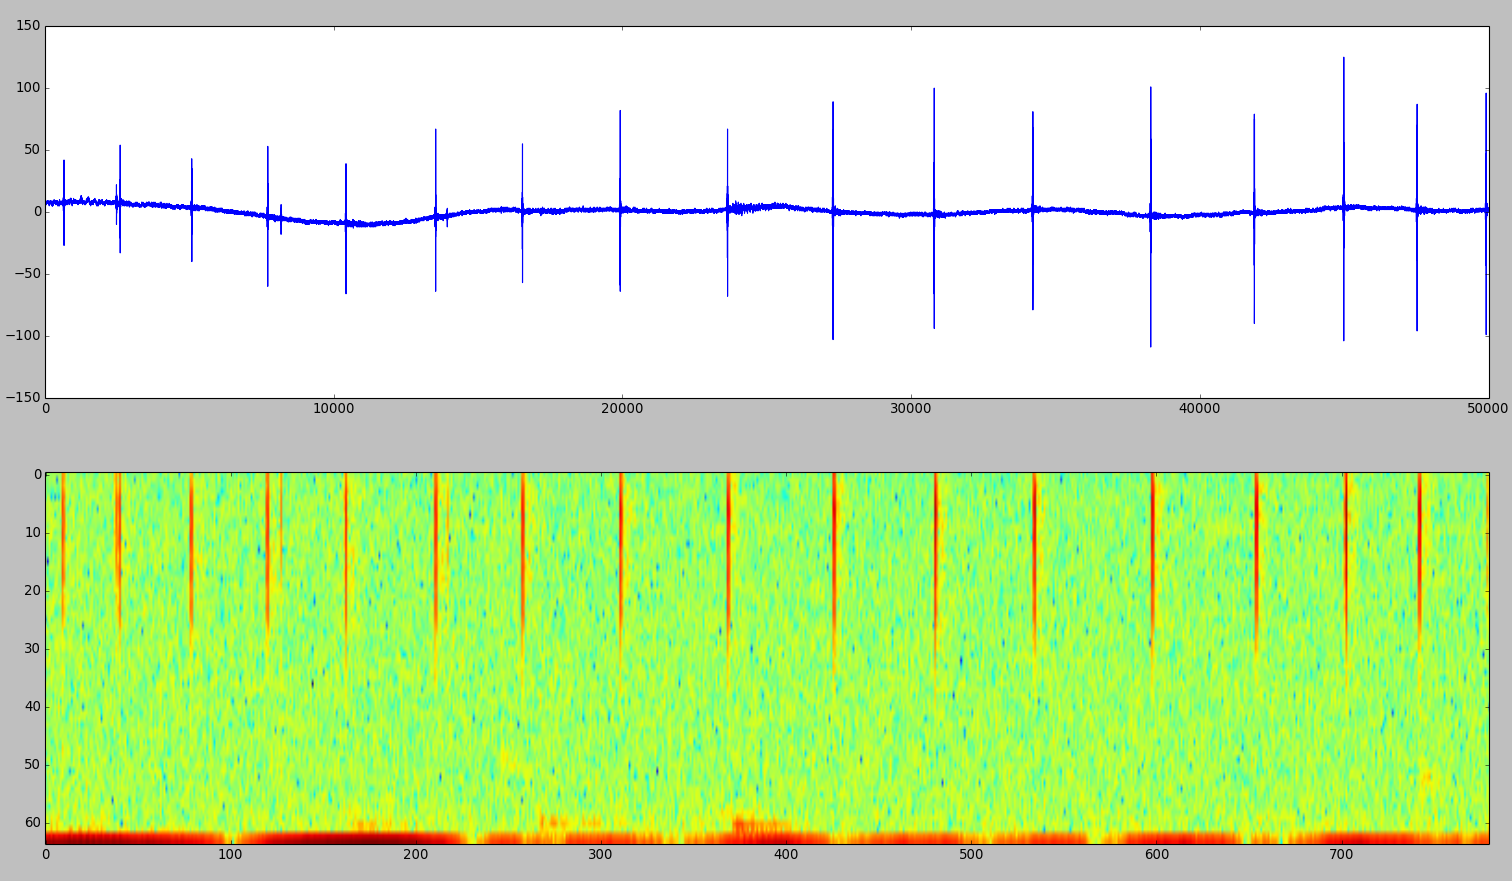
\includegraphics[scale=0.21]{fftslow.png}\caption{Inia Dolphin Slow Clicks : Spectrogram 128 50\%}
\end{center}
\end{figure}

\begin{figure}[H]
\begin{center}
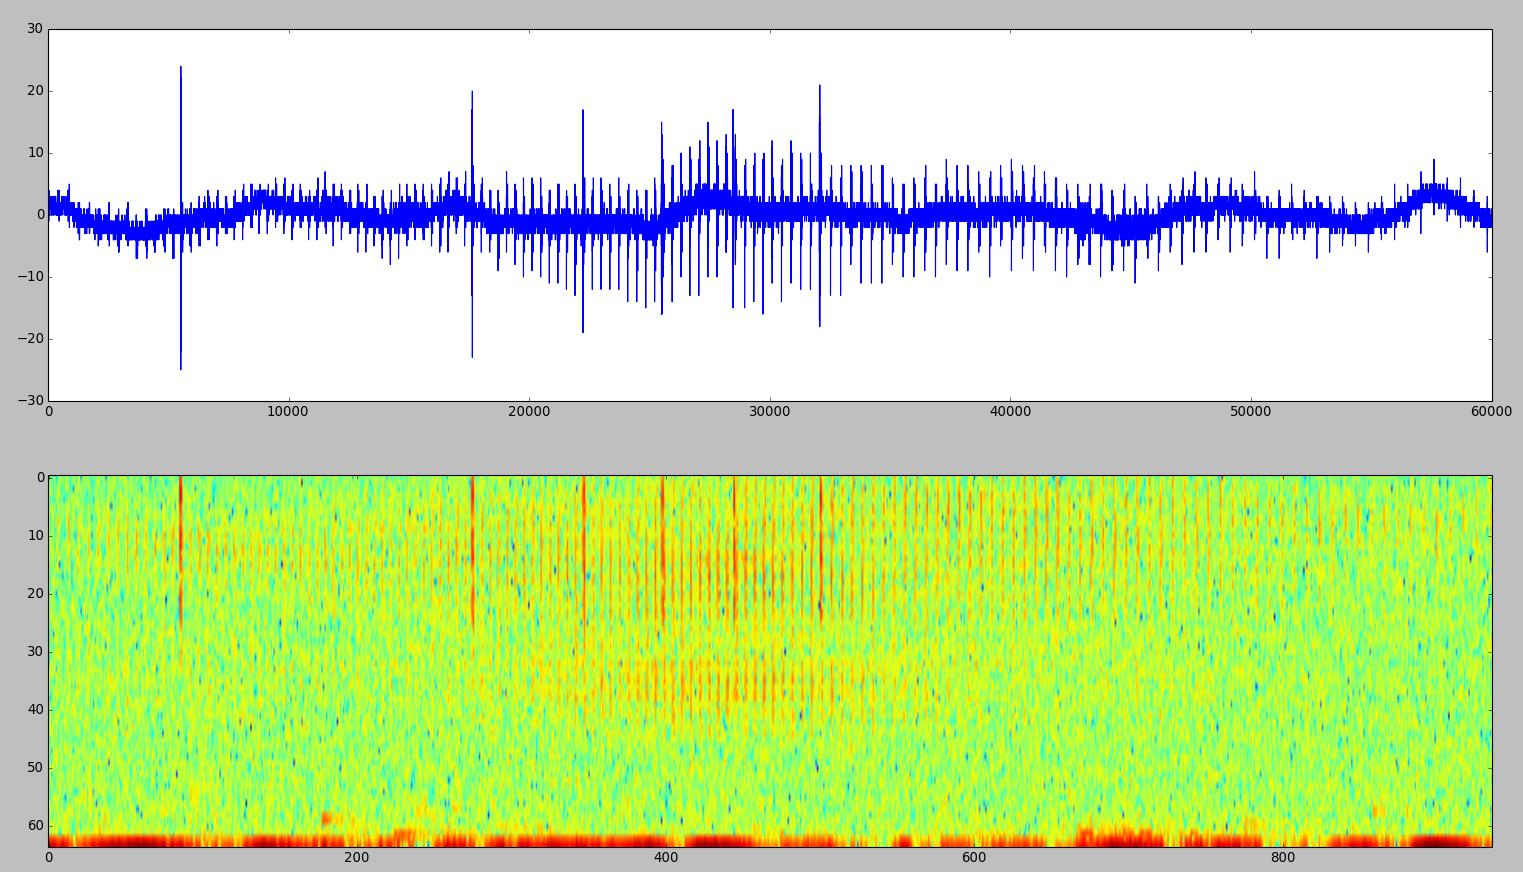
\includegraphics[scale=0.21]{fftfast.png}\caption{Inia Dolphin Fast Clicks : Spectrogram 128 50\%}
\end{center}
\end{figure}

\begin{figure}[H]
\begin{center}
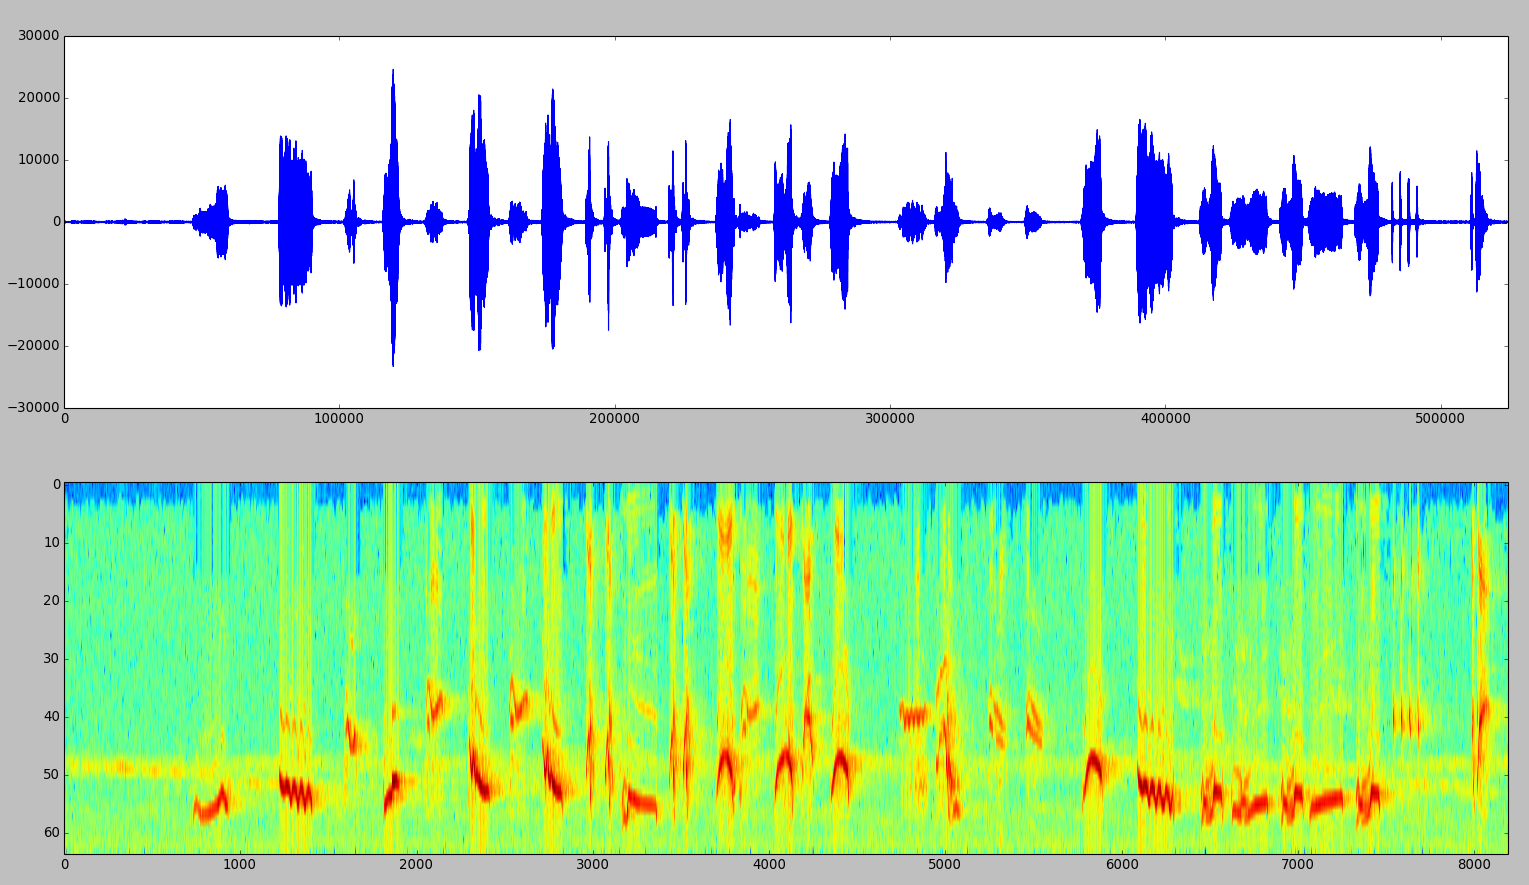
\includegraphics[scale=0.21]{fftbird.png}\caption{Bird : Spectrogram 512, 50\% }
\end{center}
\end{figure}


\chapter{Scattering Network Fast Implementation}
\section{Meta-Parameters}
In order to respect the scattering network architecture, this toolbox uses a specific structure : MetaParam using default parameters and a TtoJ method :

\begin{lstlisting}
   MetaParam L1param(500);
   //L1param._T=500, L1param._Q=1, L1param._J=8, L1param._PE=1
   L1param=MetaParam(500,2);
   //L1param._T=500, L1param._Q=2, L1param._J=6, L1param._PE=1
   L1param=MetaParam(500,2,4);
   //L1param._T=500, L1param._Q=2, L1param._J=4, L1param._PE=1
   L1param=MetaParam(500,4,4,4);
   //L1param._T=500, L1param._Q=4, L1param._J=4, L1param._PE=4
\end{lstlisting}

Let's now see the details of each implementation level and emphasize the implementation architecture used.
\section{Filter Bank Creation}
Filters are created through the constructor of the Filter1D class. Given meta-parameters and a support size, the constructor will initialize all the wanted variables and compute the actual filters. Note that the Filter1D class has two children : the MorletFilter1D and GaborFilter1D. These two specializations have their own filter generation algorithm. This also means that if one wants to implement a new filter, the only thing to do is to create another class of the name of this filter, inherit from the Filter1D class and implement the coefficients generation method.
\\Note that the constructor can be used in two different ways :
\begin{itemize}
\item Giving support size, meta parameters, and the position of the filter in this configuration ($gamma$)
\item Giving a support size, a $\sigma$ and a $\xi$.
\end{itemize}
The first is used to generated the $\psi$ filter bank and the second one for the $\phi$ filter.
\\
Here is an example with arbitrary coefficients :
\begin{lstlisting}
    Filter1D* BankFilter=new Filter1D[5];
    BankFilter[0]=GaborFilter1D(500,0,1,2);//500 points, xi=0,sigma=1,PE=2
    for(int i=1;i<5;++i)
        BankFilter[i]=MorletFilter1D(500,2+0.5*i,0.2*i);//500 points,xi=f(i),
                                                        //sigma=g(i),PE=1 (default)
    ofstream file("filters.txt");
    for(int i=0;i<5;++i){
        file<<BankFilter[i];// use of the overloaded operator
        file<<"\n";
    }
    delete[] BankFilter;
    file.close();

\end{lstlisting}
Giving the following result :
\begin{figure}[H]
\begin{center}
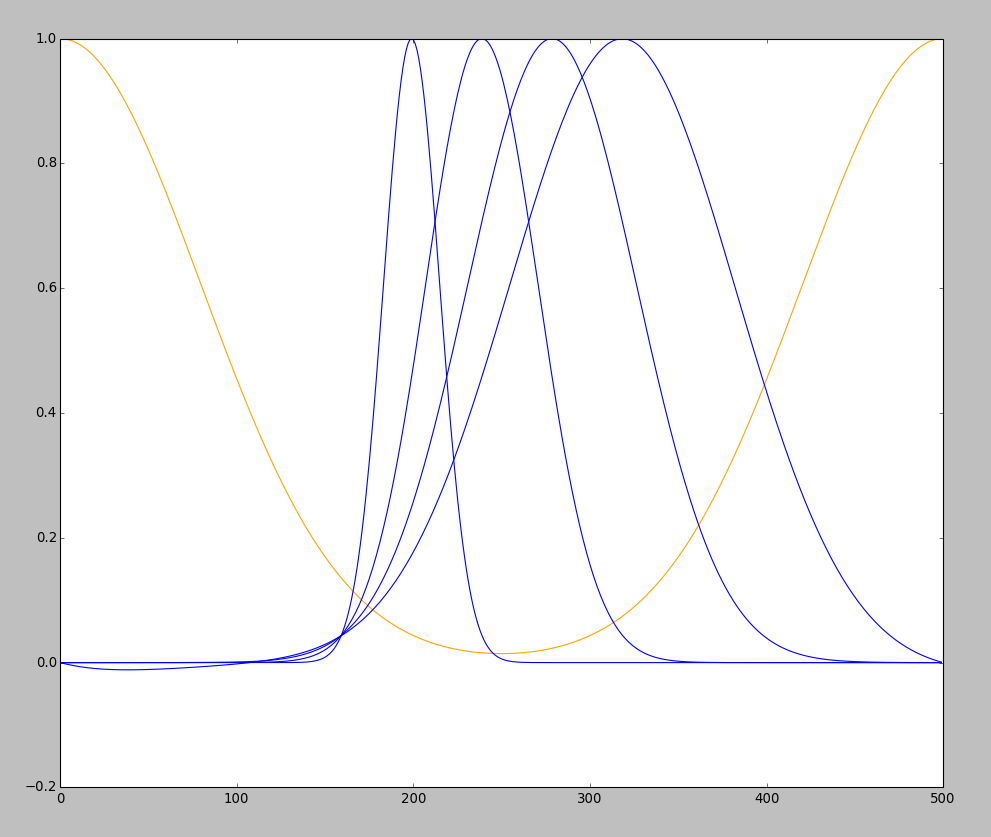
\includegraphics[scale=0.21]{example1.png}\caption{Filters generation example in the frequency domain, orange : Gabor filter, blue : Morlet wavelets.}
\end{center}
\end{figure}
Let's now look at the high-pass filter bank generated through a scattering layer :

\begin{lstlisting}
    
    MetaParam AA;
    AA._Q=8;
    AA._J=5;
    AA._T=4;
    ScatteringLayer LL;
    LL.CreatePsis(pow(2,10),AA);
    ofstream F("psis.txt");
    F<<LL._Psis;
    F.close();

\end{lstlisting}
Giving the following result :
\begin{figure}[H]
\begin{center}
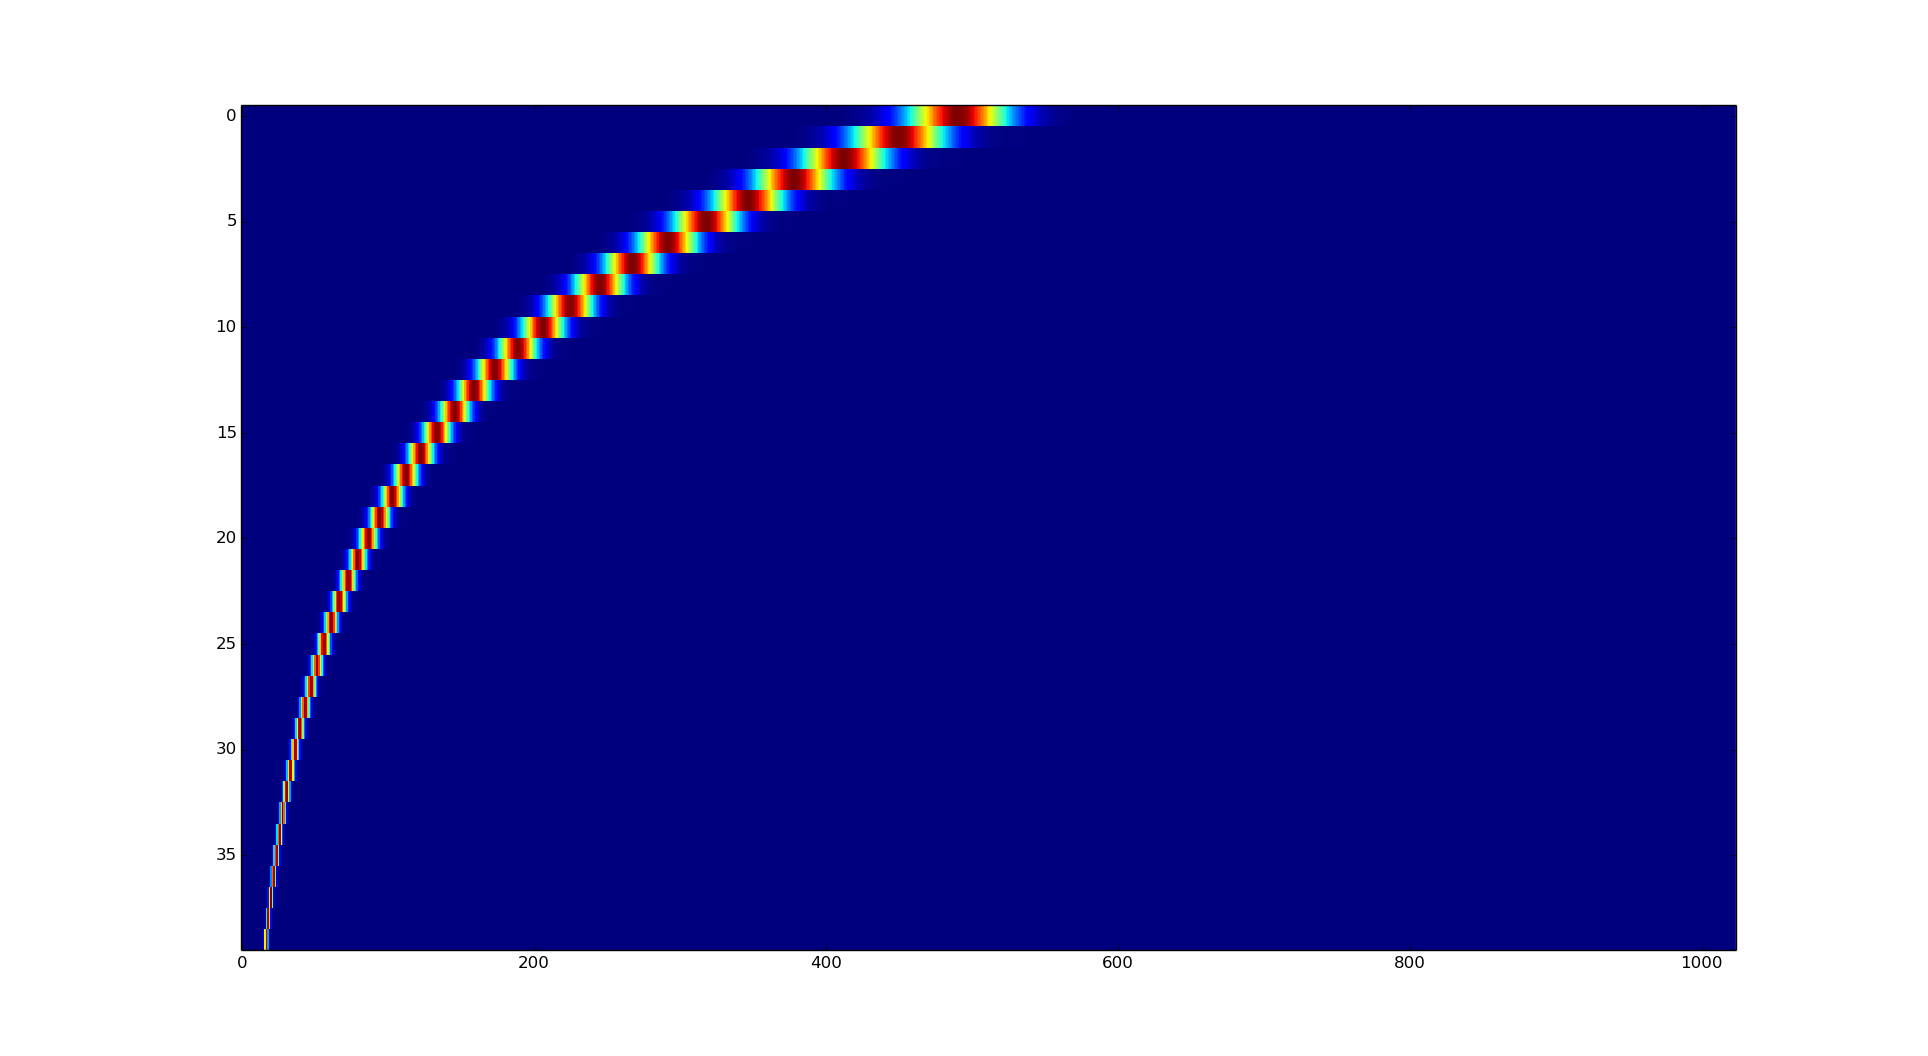
\includegraphics[scale=0.21]{psis.png}\caption{On 1024 bins, Q=8, J=5 without optimization on the support}\label{psis_examples}
\end{center}
\end{figure}
Here is the diagram summary of the layer class.
\begin{figure}[H]
\begin{center}
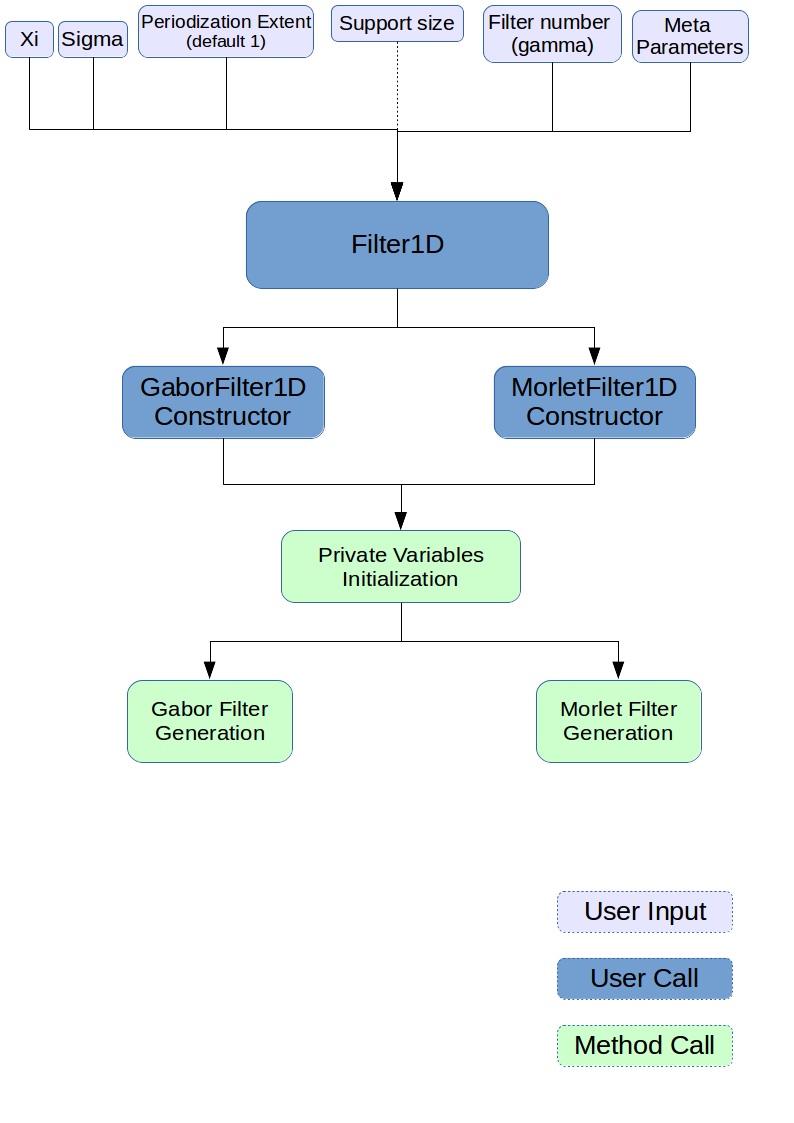
\includegraphics[scale=0.31]{filter_diagram.png}\caption{Filter1D Summary Diagram}
\end{center}
\end{figure}
\section{Layer Implementation}\label{ll}
The role of this class is to be the link between the raw input, the meta parameters, and the filter banks by performing the decomposition process. Firstly, this class takes a $2D$ input (the input signal has to be transformed for the first layer). This allows an easy link between layers by directly setting the input of the next one as the output of the previous one. 
\\
Given the input, private variables are computed determining the structure of the class by computing variables that will be passed to the next layer such as the size of the output (given the input size and the number of $\psi$ filters :$Q*J$). Then when all the $\psi$ filters are available a Littlewood-Paley normalization is performed (due to the logarithmic spaced filters). After this, the filters are generated using the Filter1D class. The Decomposition can now be performed.
\\
Note that the decomposition is stored as a $2D$ matrix for every layer. Normally, layer $i$ has a dimension of $i+1$ which is not true in term of memory management. In fact, in this toolbox, the graph structure of the scattering network\ref{oo} has been kept through $2D$ matrices. For example for the second layer if we have $|\lambda_1|$ filters for the first layer and $|\lambda_2|$ filters for the second layer, the $U_2$ matrix of will be :
\[ U_2:= \left( \begin{array}{c}
||x \star \psi_{1,1}|\star \psi_{2,1}|\\
||x \star \psi_{1,2}|\star \psi_{2,1}|\\
\dots \\
||x \star \psi_{1,|\lambda_1|}|\star \psi_{2,1}|\\
||x \star \psi_{1,1}|\star \psi_{2,2}|\\
||x \star \psi_{1,2}|\star \psi_{2,2}|\\
\dots \\
||x \star \psi_{1,|\lambda_1|}|\star \psi_{2,2}|\\
\dots \\
||x \star \psi_{1,1}|\star \psi_{2,|\lambda_2|}|\\
||x \star \psi_{1,2}|\star \psi_{2,|\lambda_2|}|\\
\dots \\
||x \star \psi_{1,|\lambda_1|}|\star \psi_{2,|\lambda_2|}|\\
\end{array} \right)\]

Here is a summary of the scattering layer graph.
\begin{figure}[H]
\begin{center}
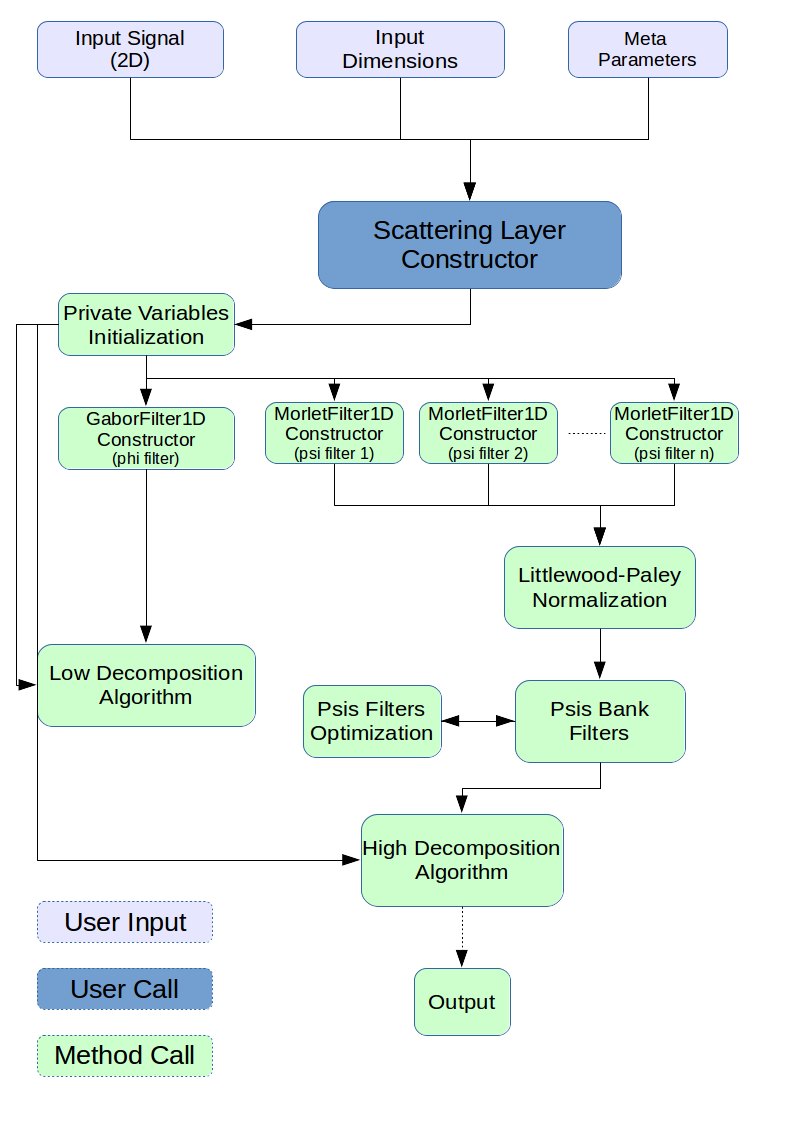
\includegraphics[scale=0.40]{layer_diagram.png}\caption{Scattering Layer Summary Diagram}
\end{center}
\end{figure}

\section{Scattering Network Implementation}
Finally here is how to perform the Scattering Network on a signal and to save the outputs :
\begin{lstlisting}
    MetaParam* opt=new MetaParam[3];
    opt[0]=MetaParam(8,30,4,1);
    opt[1]=MetaParam(64,1,1,1);
    opt[2]=MetaParam(1024,1,1,1);
    ScatteringNetwork decomposition("signal.wav",opt,3);

    ofstream file;
    file.open("layer1.txt");
    file<<decomposition[0];
    file.close();
    file.open("layer2.txt");
    file<<decomposition[1];
    file.close();
    file.open("layer3.txt");
    file<<decomposition[2];
    file.close();
    delete[] opt;
\end{lstlisting}
In fact the operator [] is overloaded to return the specific layer which itself uses its overloaded operator to export the coefficients.
\begin{figure}[H]
\begin{center}
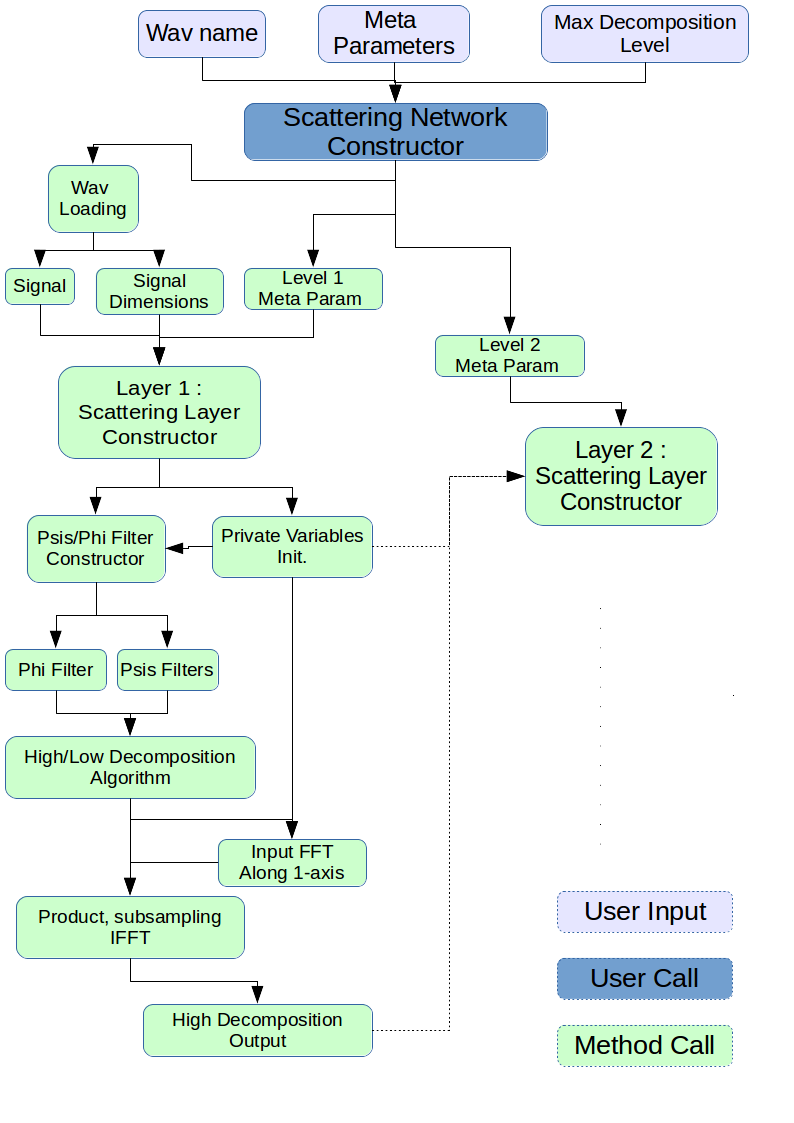
\includegraphics[scale=0.38]{scatteering_diagram.png}\caption{Scattering Network Summary Diagram}
\end{center}
\end{figure}
\section{Optimizations and Computation Time}
\subsection{Filter Bank Optimizations}
Since we want to use this implementation on massive dataset, it is mandatory to optimize the implementation.

The best way to improve the required time to perform the decomposition is around the filters (allocation, creation, application,...). In fact, FFT/IFFT and the periodization algorithms already use efficient algorithms. 


I present here only the improvements concerning the filter bank, other details can be found in the C++ file comments.\\ 
The first big improvement is to only save in memory the coefficients of the filters that are not zero. So by only keeping the support of $\psi$ we can save memory but more importantly when we apply the operation $inputFFT .* \psi_{L,i}$ we only need to perform it on the support and set all the other coefficients to $0$. Doing this is really efficient by the natural sparsity of the filters as shown here : \ref{psis_examples}.
\\
Now that we only save part of the coefficients, the dimension is reduced and it is even possible to optimize again the filters creation. We know that filters are completely determined by the size of the input $N$ and the meta parameters $Q$ and $J$ for the $\psi$ filters. So in other word, it is possible to create a filter bank dictionary and save them in .txt files thus when we need some filters we only need to load them and not explicitly compute them over and over. This is particularly true since the input size must be a power of $2$ so there are not a huge number of input size that we can take as input.
By doing so, when we treat for example thousands of files, we will only load a few files without having to recompute the filters coefficients every single time.
Now, if we use the implementation in a loop over several signals, it is even possible to first load the filters and then perform all the decomposition without having to load filters every time too ! 
\\Note however that this optimization is not always usable. In fact, the use of this toolbox on other platform/servers or just because the user doesn't want IO operations for example, requires to actually compute the filters every time. In this case, the generating algorithm has been optimized using standard C++ optimization techniques such as loop-unrolling, inplace methods,...

\subsection{Computation Time}

Using all the available optimization without the use of the filter bank IO (thus generating the filters every time) this toolbox needs about $30\%$ of the signal duration (in second) to perform the loading of the wav, scattering decomposition and saving of the scattering coefficients into a .txt files). This required time obviously varies with the meta-parameters, the ones use here are the common ones (also used for the classification challenge presented later).
Note that using the filter bank IO will lead to better performance on huge dataset by not recomputing the filters for every signal.
The Scatnet implementation available in matlab requires $400\%$ of the signal time to perform the decomposition algorithm.
\\
Note that this toolbox is now used as the reference implementation for the scattering decomposition on ENS and UTLN servers for massive dataset decomposition (such as bioacoustic challenges). 
\section{Examples}
In the examples below we did not apply any operation (logarithm, re-normalization,...). The sub-plots are from top to bottom the
signal, and the $U_1$, $U_2$, $U_3$.
\begin{figure}[H]
\begin{center}
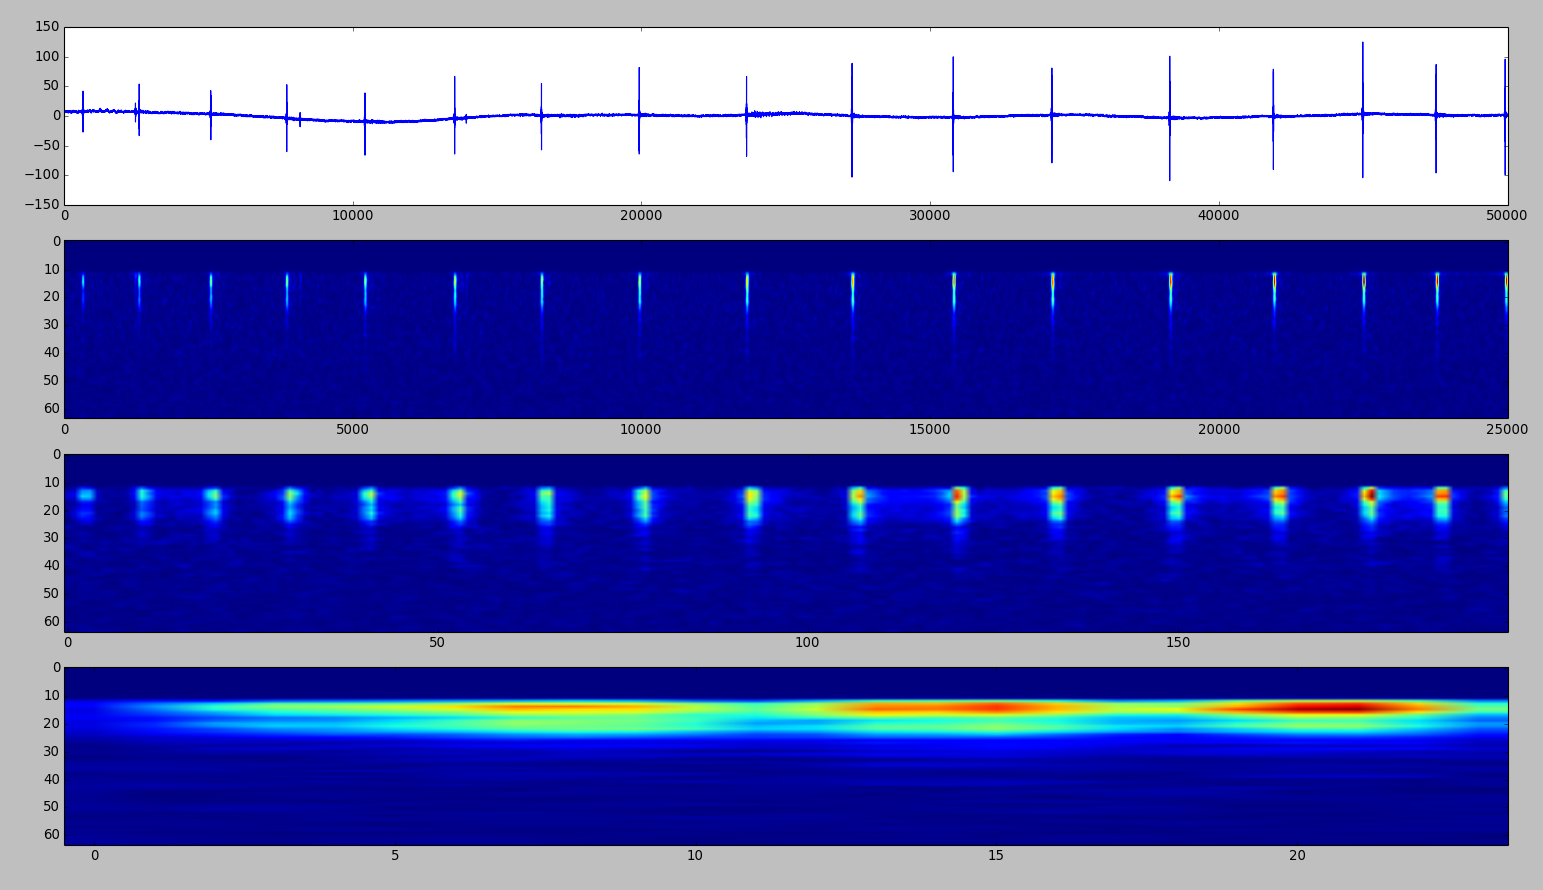
\includegraphics[scale=0.21]{slow.png}\caption{Signal (waveform), $U_1$, $U_2$, $U_3$ of Inia Perou \cite{trone2015}, a dolphin (slow clicks) T1:4 Q1:32 J1:2 T2:256 Q2:1 J2:1 T3:16 Q3:1 J3:1}
\end{center}
\end{figure}

\begin{figure}[H]
\begin{center}
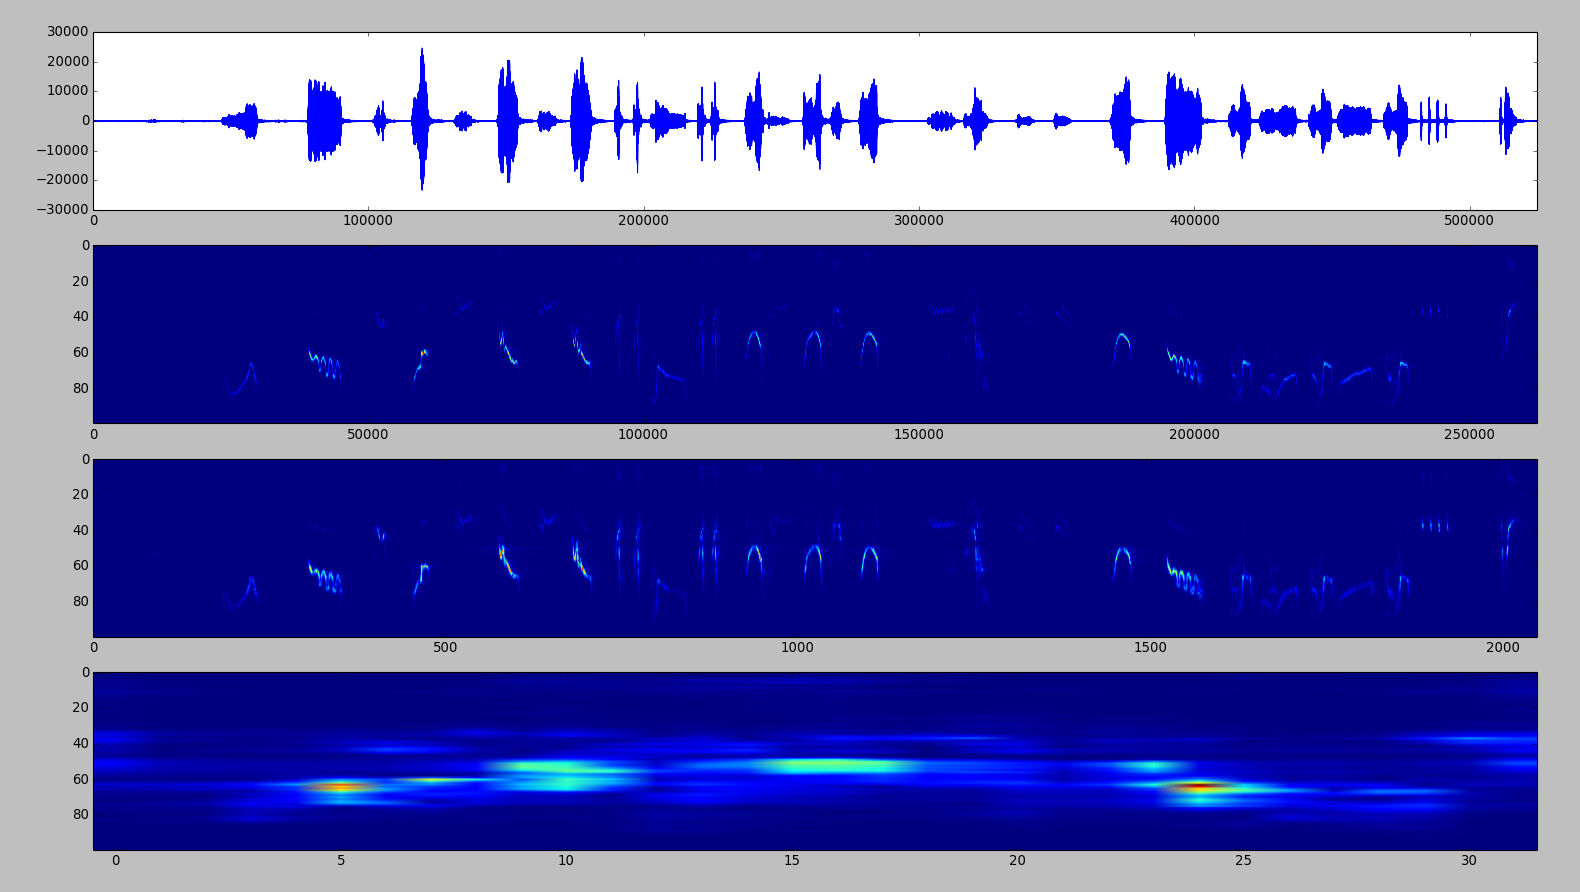
\includegraphics[scale=0.21]{bird.png}\caption{Signal (waveform), $U_1$, $U_2$, $U_3$ Bird (BIRDLIFE CLEF Challenge) T1:4 Q1:25 J1:4 T2:256 Q2:1 J2:1 T3:128 Q3:1 J3:1}
\end{center}
\end{figure}
\part{Benchmark and Bioacoustic Classification}

\chapter{Challenge Presentation}

\section{Description}

The task is focused on bird identification based on different types of audio records over 999 species from South America centered on Brazil. Additional information includes contextual meta-data (author, date, locality name, comment, quality rates). The main originality of this data is that it was built through a citizen sciences initiative conducted by Xeno-canto, an international social network of amateur and expert ornithologists. This makes the task closer to the conditions of a real-world application: (i) audio records of the same species are coming from distinct birds living in distinct areas (ii) audio records by different users that might not used the same combination of microphones and portable recorders (iii) audio records are taken at different periods in the year and different hours of a day involving different background noise (other bird species, insect chirping, etc).


The data is built from the outstanding Xeno-canto collaborative database (http://www.xeno-canto.org/) involving at the time of writing more than 192k audio records covering 9120 bird species observed all around the world thanks to the active work of more than 2020 contributors.

The subset of Xeno-canto data that will be used for the first year of the task will contain 33203 audio recordings belonging to the 999 bird species having the more recordings in the union of Brazil, Colombia, Venezuela, Guyana, Suriname and French Guiana Xeno-canto recordings. The amount of 999 classes will clearly go one step further previous benchmarks (80 species max) and foster brave new techniques. On the other side, the task will remain feasible with current approaches in terms of the number of records per species and the required hardware to process that data. Detailed statistics are the following:
\begin{itemize}
\item minimally $14$ recordings per species (maximum $>200$)
\item minimally $10$ different recordists, maximally $>40$, per species.
\end{itemize}
The last year challenge used MAP in order to rank the different submissions. In fact, by the difficulty of this challenge, just computing the accuracy is too strict for results comparison. The MAP is always greater than the exact accuracy. The best submission last year reached a MAP of about $35\%$ for our case (on the set without using meta data or using only signals without background noises).


This Challenge is organized by Pr. Glotin, Pr. Joly and Xeno Canto since 2014 following Challenges launched by Pr. Glotin and al. for NIPS4B 2013, ICML4B 2013 which were under the massive dataset project MI CNRS MASTODONS in the Scaled Acoustic Biodiversity project.
SABIOD.ORG is organized by Pr. Glotin (UTLN) now with the collaboration of LifeClef (Clef Challenge).
\section{Problem Approach}

The goal of any classification task is to find a way to learn (not necessarily in a supervised way) the underlying structures of the data in order to then generalize it for classification of unseen examples. In our case, we start with a set (the training set) made of raw signals (vectors) and corresponding labels (scalars): $(\textbf{x},\textbf{y})$.\\
Our goal is then to find a classification process $f$ from the input space to the set of labels $\textbf{X}\rightarrow \textbf{Y}$ such that when given a new unseen example $x$, $f(x)$ predicts it belonging class (with a certain confidence). This process is usually a multi-step algorithm, first mapping data into new spaces where we can then more easily apply a classification algorithm. In fact, the classification can become really natural when the given classes are already linearly separable. In our case though, this is not naturally the case. A simple approach is to first find a new (more informative) representation of the signals into a new space. By doing so we wish to gain discriminative information while reducing the non informative variance (through denoising for example). This kind of transformation can be done in cascade by using different algorithms, but in the end we want to have mapped the data into a new space where examples from the same class will be similarly represented and data from different classes will be easily separable. The classification is then trivial and this is why we will focus our analysis on the preprocessing part and try to show its key role in the whole classification task.
\\
\\
\begin{tabular}{l c}
$Input:=x$ &
\begin{tabular}{|c|}
\hline
Raw Data (wav file) \\
\hline
\end{tabular}\\
&$\downarrow$\\
$Preprocessing:=g(x)$ & \begin{tabular}{|c|c|}
\hline
Denoising&Transformation\\
\hline
\end{tabular}\\
&$\downarrow$\\
$Feature Selection:=f(g(x))$ & \begin{tabular}{|c|c|}
\hline
Dimensionality Reduction & Feature Selection\\
\hline
\end{tabular}\\
&$\downarrow $\\
$Prediction:=y=p(f(g(x)))$&
\begin{tabular}{|c|}
\hline
Classification \\
\hline
\end{tabular}
\end{tabular}
\paragraph{Input}
The input in this task is the raw wav file recorded with a sampling frequency of $48000$ Hz. Recording devices are not necessarily the same and signals structures are different (background noises, geographic locality, recorder quality ,...). The lengths of the signals are also really unequal (from $0.1$ second to $45$ min) and the ratio of the bird presence over the signal length is inconsistent from signal to signal. This already can highlight some questions regarding the data to keep for the training phase. For example, including the $0.1s$ long signal could actually make the classifier less efficient overall. At the same time, including the $45$-minute long signal could make it overfit this class.
\paragraph{Preprocessing}
The key part of our approach concerns the preprocessing part and more specifically the scattering network architecture and the use of its coefficients. On the other hand,  denoising will be part of it so our whole preprocessing part will be made of the scattering network.
\paragraph{Feature Selection}
By the use of the scattering network, the features that we will use are simple statistics of the coefficients computed by row meaning that for the first layer for example,  we will analyse each row $i$ with $|x \star \psi_{1,i}|\star \phi_1$ independently from each other. Each vector will be of different lengths from signal to signal thus only taking statistics such as the max aggregates the time component. This is obviously not optimal and the use of other features could lead to better results.\\
It is know possible to analyse each vector by a "vertical" component with the Joint-Scattering that has just been developed by the ENS team and that will be published soon.
\paragraph{Prediction}
Finally the classification will be made using a two-layer perceptron (with a multinomial logistic regression for class prediction in the end). This classifier will only be optimized through the number of hidden nodes for the hidden layer.\\
Note that other approaches are possible, this could be made with SVM, random forests,...
\paragraph{Sub-training set}
This is obviously not possible to test algorithms on the whole training set since it could need weeks to be trained. The common approach is to create a sub-training set where tests are made. This puts a condition : this set has to be representative and has to include all the difficulties and most of the special cases of the task. This has been done for example for image classification where algorithms are trained on CIFAR10 to then be generalized to the CIFAR100 challenge.
We will use a sub-training set of $45$ classes each one having $15$ examples. 
\paragraph{Comments}
The use of a MLP means that lots of fine-tuning can be done (L1/L2 norm conditions,learning rate,batch size,...) but our focus here remains on the preprocessing part and how can we find a good mapping for a bioacoustic dataset.

\section{Informative Features Analysis}
The goal is to first analyse the features we are interested in. By doing so we will be able to understand the communication behaviours we are trying to capture and the difficulties in this task. This will also show that this kind of approach is ad-hoc. A good way to do this is to try to build an automatic (deterministic) feature extractor. By the general aspect of this challenge ($1000$ species) it won't be possible to provide an efficient feature extractor but the analysis will still remain informative.
\\
We will be working on the first layer high-decomposition ($U_1$). We first have some requirements about this extractor : it has to have a low complexity (close to linear) and the algorithm has to assume no prior knowledge (on the bird behaviours, the recording device, the environment,...).
\\
With the scattering transform, new data representations are sparse. We will use this to produce a "robust" and general feature extractor. The aim is to have a "no-tweaking" technique working equally good on every class.
 The only assumptions are :
\begin{itemize}

\item (relatively) Sparse Scalograms (easiest feature extraction)
\item Given a frequency domain, the most present specie in it is the one of interest
\end{itemize} 

This algorithm is made of two parts. The first one is simply a reconditioning of the scalogram in order to improve the second part performance : the feature extraction. One can see the analogy with the classification task. We first denoise and pre-process to then classify. In fact, doing a feature extractor can be seen as a bi-class classification process where for each small time window we say if we have a bird or not.
\\
I will present all the methods, examples are given in the end in order to show the computed statistics and features.
\subsection{Row Conditioning}
\subsubsection{Non biological sound suppression}
First we will remove background and non biological noises in the scalogram. In order to do this we will simply compute row median and row standard deviation. The ones with a higher median than the standard deviation are set to $0$. Meaning that if a line has almost constant values in time without any fluctuation then it is likely to be non biological thus we suppress it.
\subsubsection{Row weighting}
The scalogram is now cleaner but can still contain biological but non bird sounds. We then wish to emphasize one from the other or at least create enough contrast between them so the features extracted in the next step are the ones of interest. In order to do so we will perform row-weighting with a coefficient computed by line and corresponding to the frequency modulation over time (the standard deviation). In fact birds are not known for having no frequency modulations in their calls.
\subsection{Word Extraction}
Now we assume that we have a "clean" scalogram with only birds or species having alike communication behaviours. We are now ready to perform the word extraction. Note that we first perform word extraction and then compute song extraction which will be based on this part. A song can be made of one or more words but we assume that we need the song for classification since only words don't fully characterize the specie. This is like a speech recognition problem where we first extract phonemes but these are not enough if we don't know how they are used and the apparition order (so we can't treat them independently).
\\
The concept is really simple and is actually taken from finance with buying and selling signals. We first take the column max (this gives us a vector where the frequency information is aggregated through the max). Now we will treat it as a time serie and thus we will apply known algorithms for determining buy/sell signals which will correspond to start/stop time window of the bird words.\\
Thus, we will first take a long simple moving average (here on $1000$ coefficients). Then, on this, we compute a smaller exponential moving average (of half the previous size, so $500$ coefficients). We normalize the result and this will give the indicator line.
\\
Now we take the exponential moving average of this indicator line (of size $1000+500=1500$). This will be our signal line.
\\
The concept is simple, whenever the indicator line crosses its signal line by moving upward, this is a buy signal. When the indicator line crosses the signal line by moving downward, it is a sell signal.
\\
In order to avoid small noisy signals we also set an automatically selected minimum value for the signal line based on its histogram.
This is mainly to avoid small disturbing signals when the scalogram is empty for a long period of time and so the two lines (indicator and signal) will become so close that a little bump in the indicator line will trigger a buy signal.
\\
This can be seen as a modified Moving Average Convergence Divergence indicator where buying and selling signals are actually start and end point of the words.
\subsection{Song Extraction}
Now we have a word decomposition of the signal. In order to find out the position of the songs (which can be composed of multiple words) we will simply analyse the repartition of the words. Let's then look at the intervals (standard deviation) between the words. Given this we will look at each word and if they are closer than two times the standard deviation from each other, we will concatenate them into a song. Note that a maximum step is set to $10000$ here so $1/4 s$ assuming that inside a song there should not be more than $1/4 s$ duration of silence.
\subsection{Examples}
Keep in mind that there are almost no false negative, only false positive. This can be easily corrected by any further feature selection. For example, just by looking at the variance inside the words extracted we can tell which ones are the wrong ones from the real ones.\\
In the following images you have from top to bottom :

\begin{itemize}\label{LEGENDA}
\item Raw scalogram with detection
\item Scalogram after denoising
\item Scalogram after line weighting
\item The lines for the detection
\item Word detector
\item song detector after word reunion
\end{itemize}

\begin{figure}[H]
\begin{center}
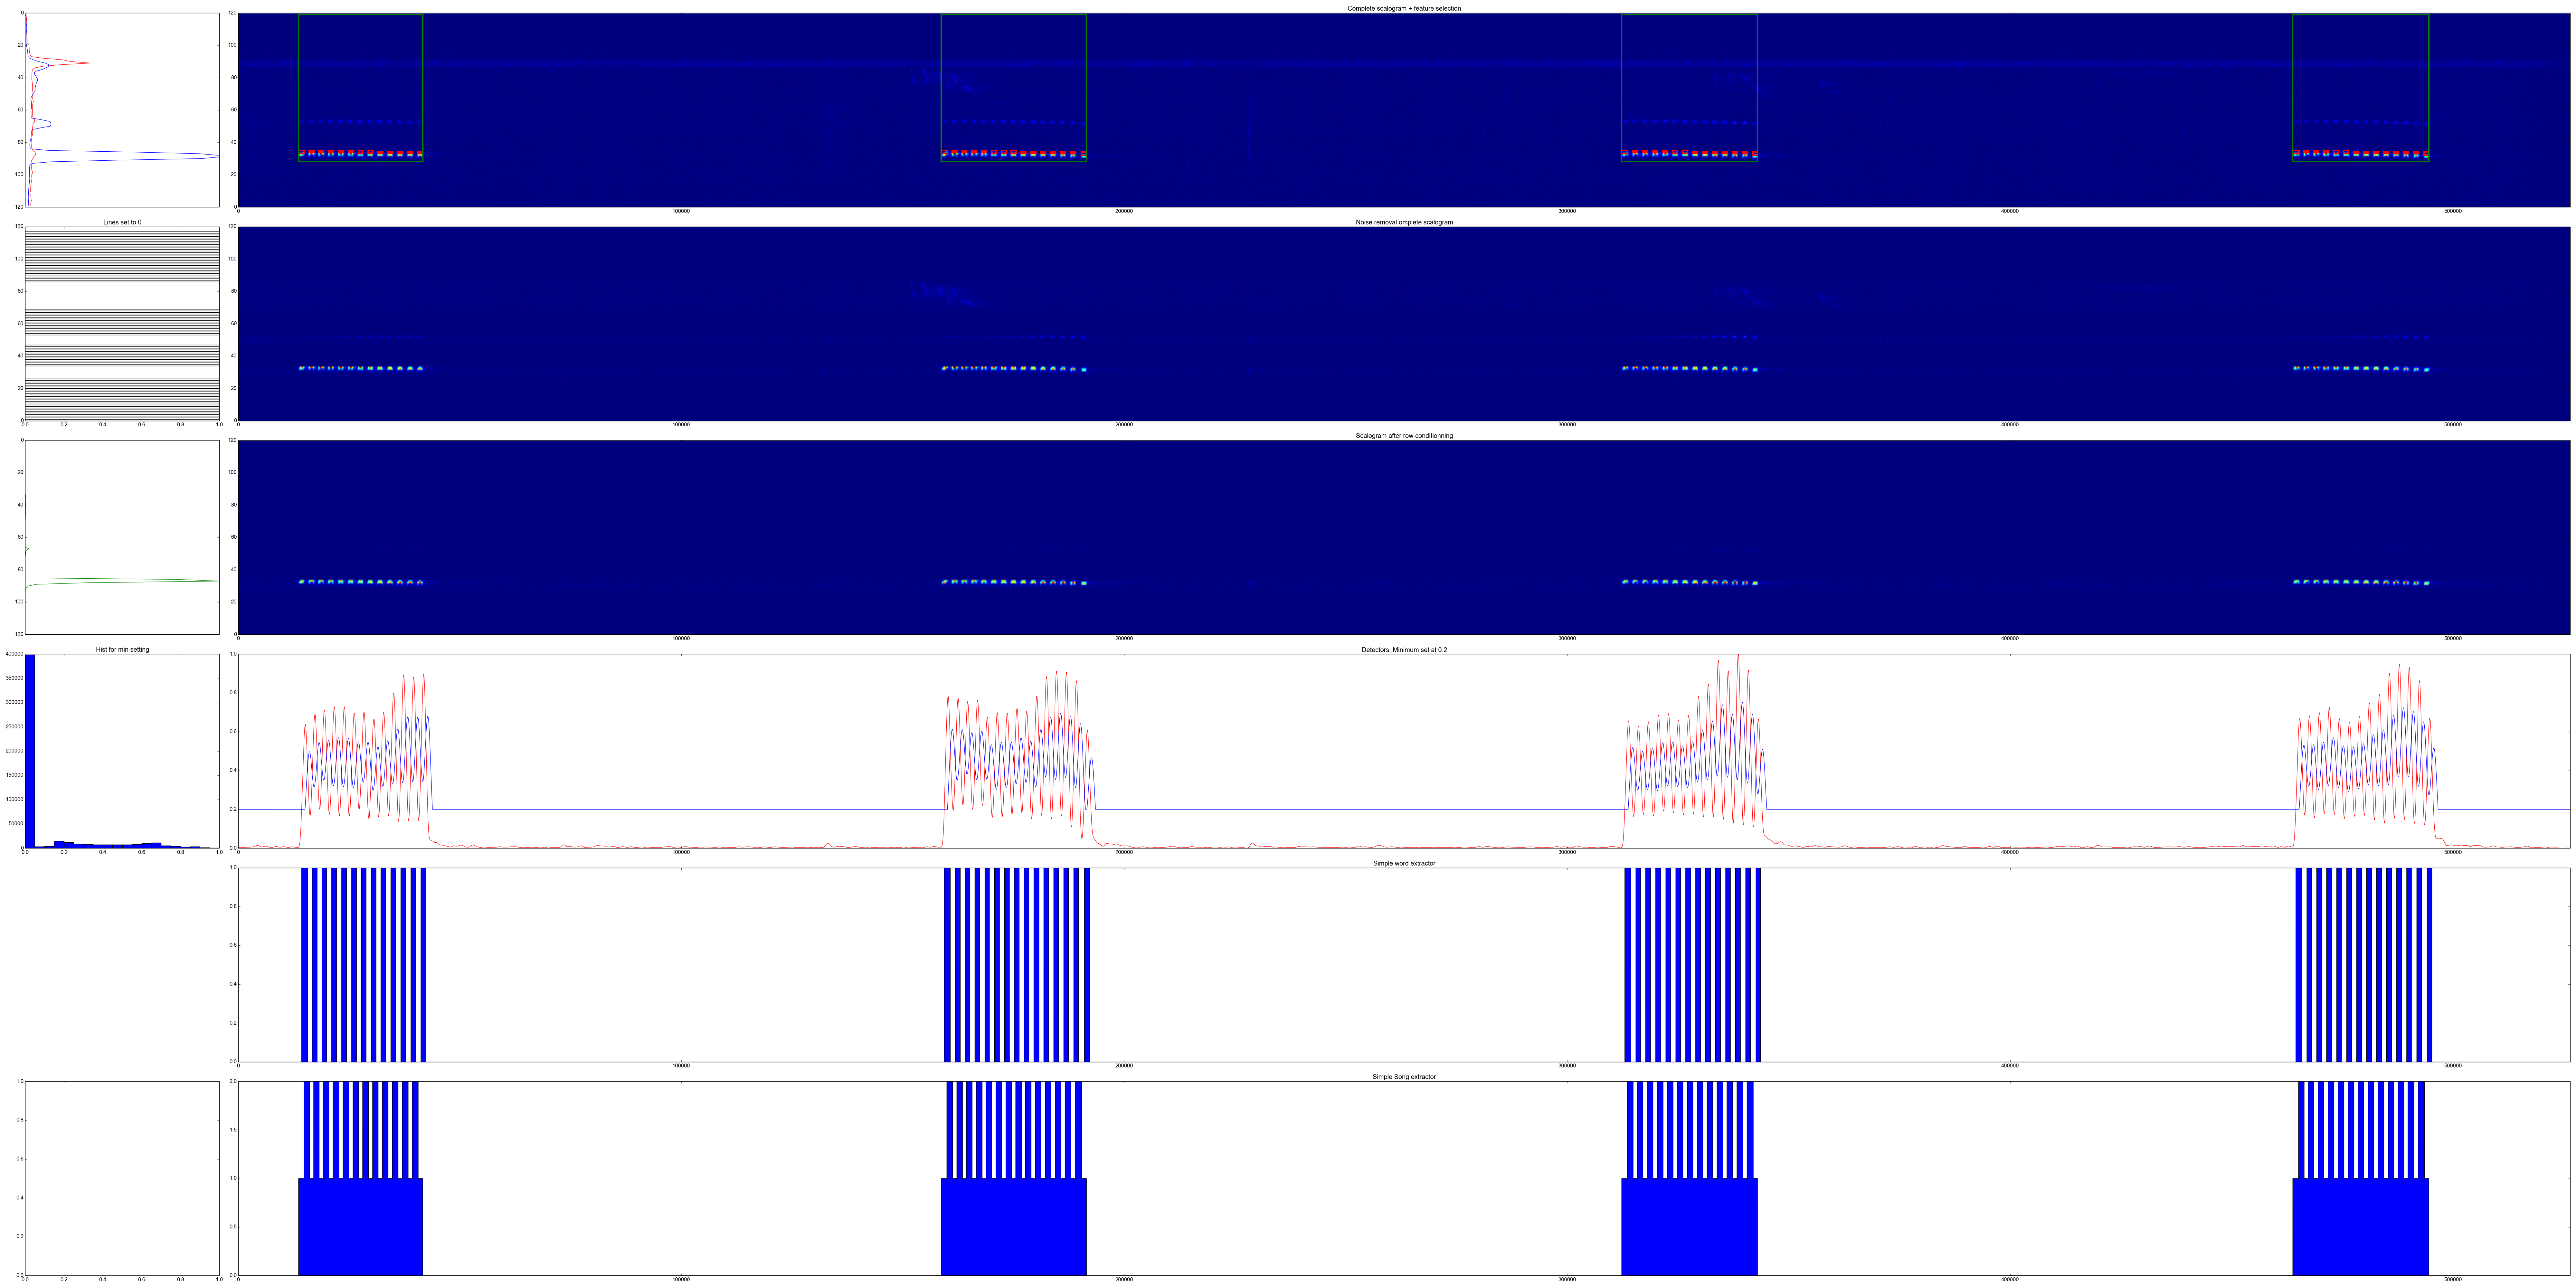
\includegraphics[scale=0.07]{1test.png}\caption{Signal : RN7917.wav with application of the automatic feature extractor, each subplot represents : \ref{LEGENDA} }
\end{center}
\end{figure}


\begin{figure}[H]
\begin{center}
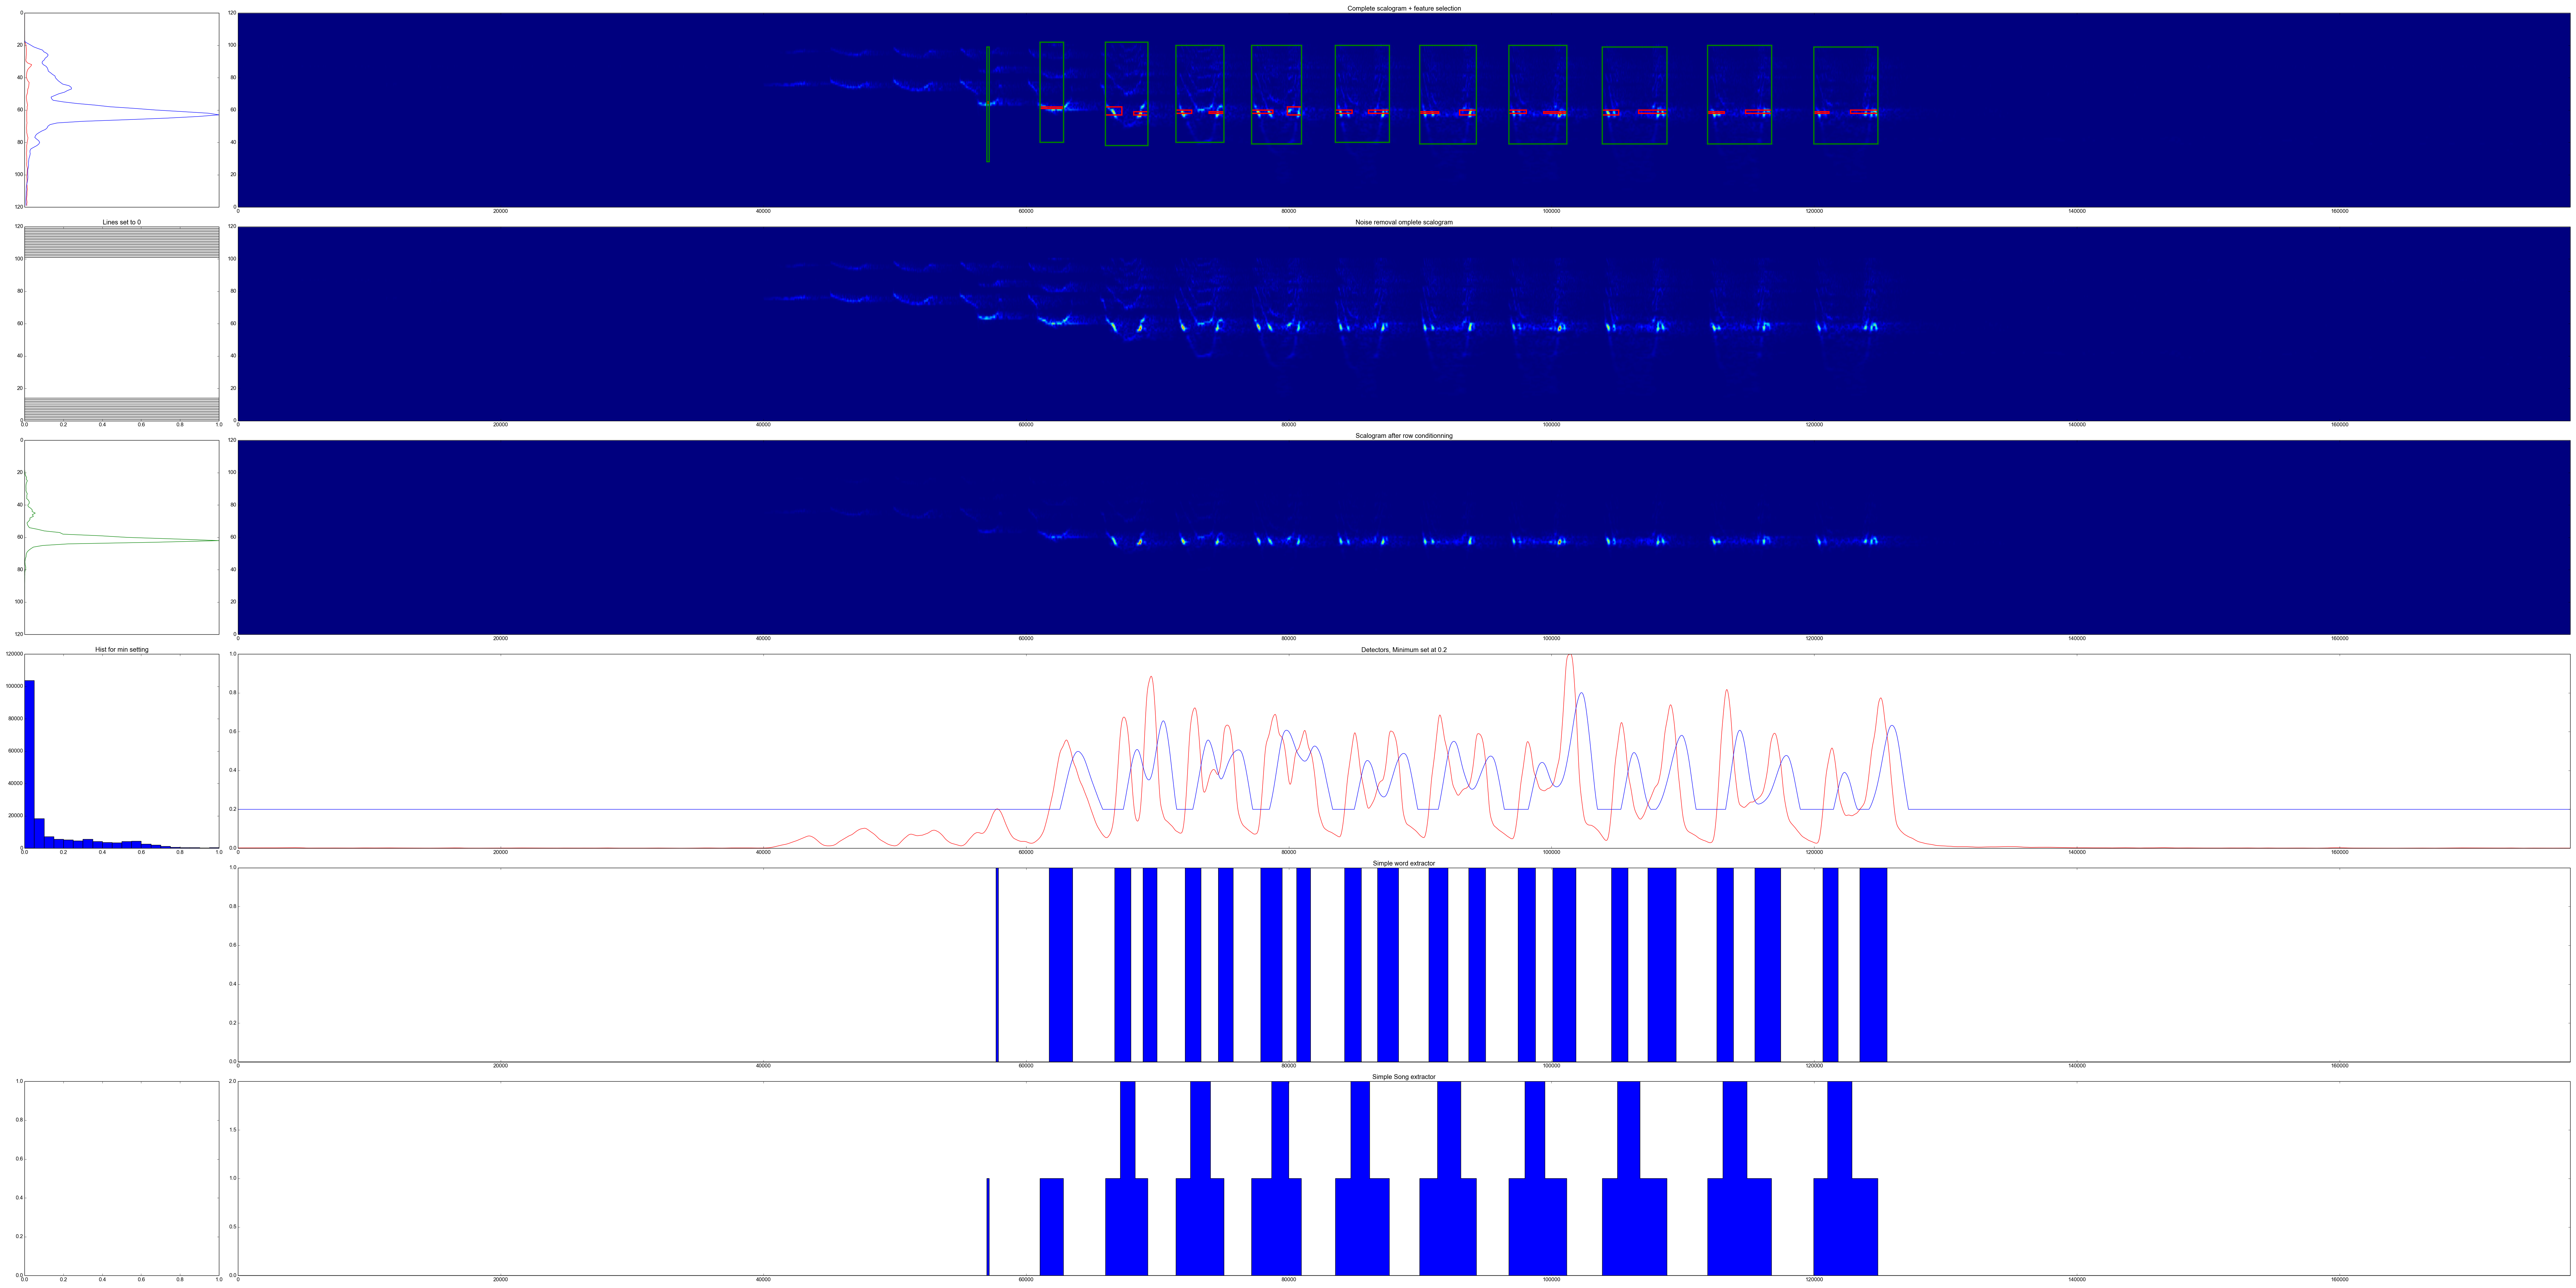
\includegraphics[scale=0.07]{2test.png}\caption{Signal : RN2320.wav with application of the automatic feature extractor, each subplot represents : \ref{LEGENDA} }
\end{center}
\end{figure}


\begin{figure}[H]
\begin{center}
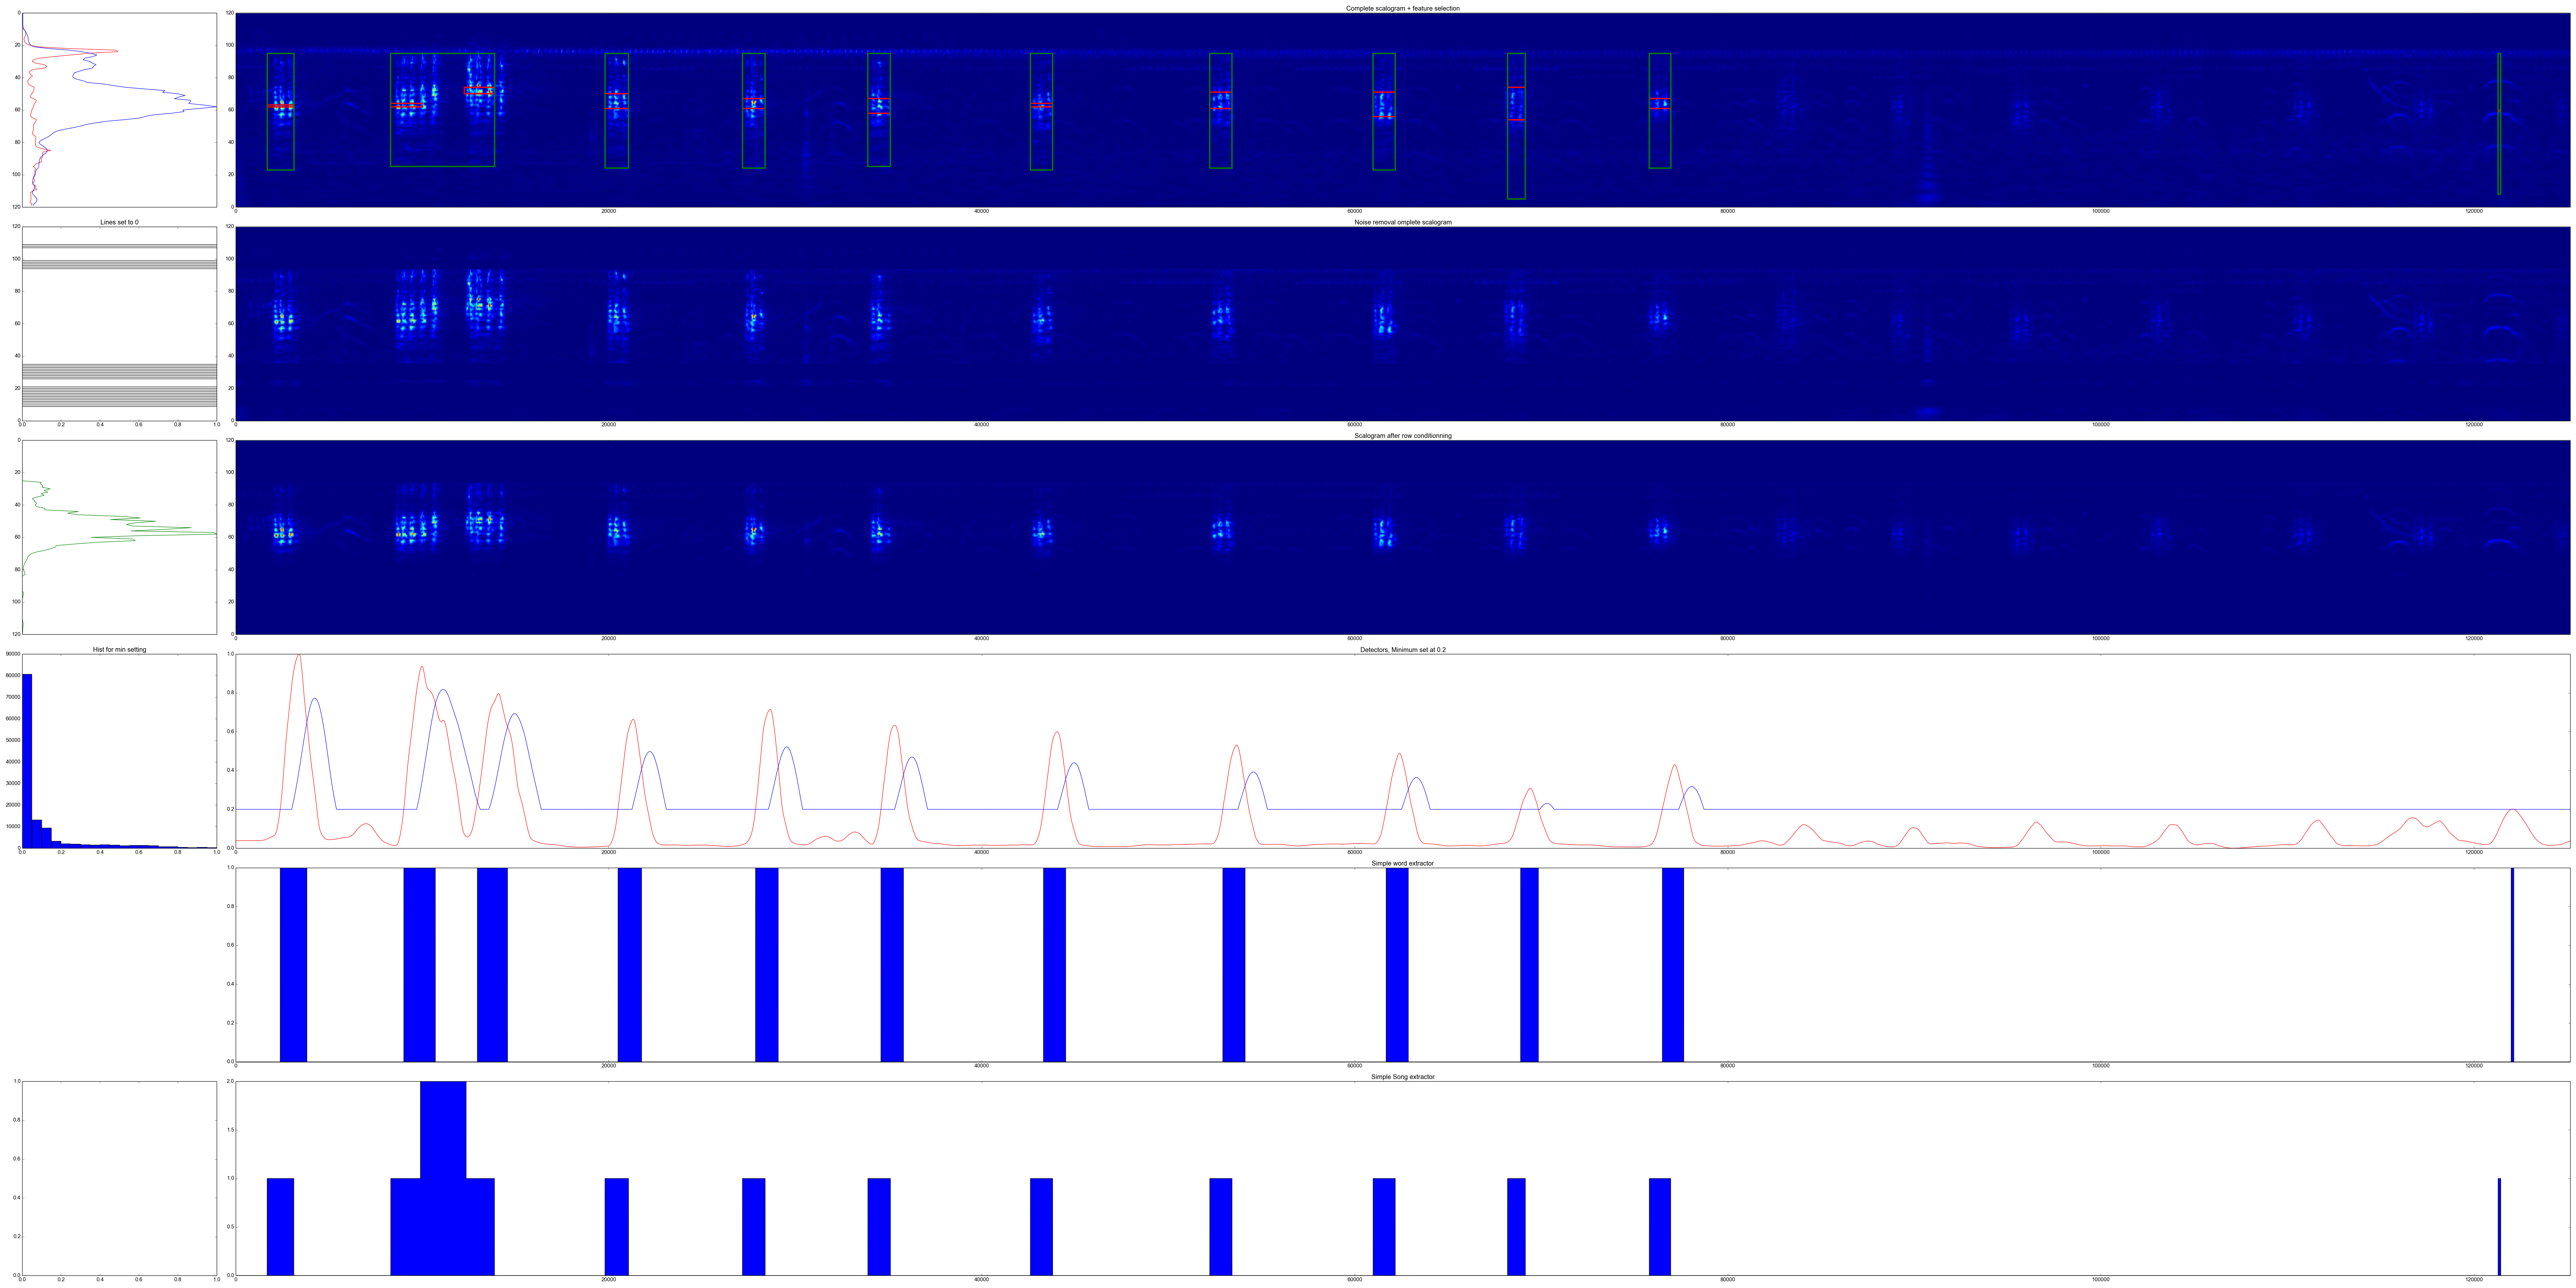
\includegraphics[scale=0.07]{3test.png}\caption{Signal : RN22.wav with application of the automatic feature extractor, each subplot represents : \ref{LEGENDA} }
\end{center}
\end{figure}


\begin{figure}[H]
\begin{center}
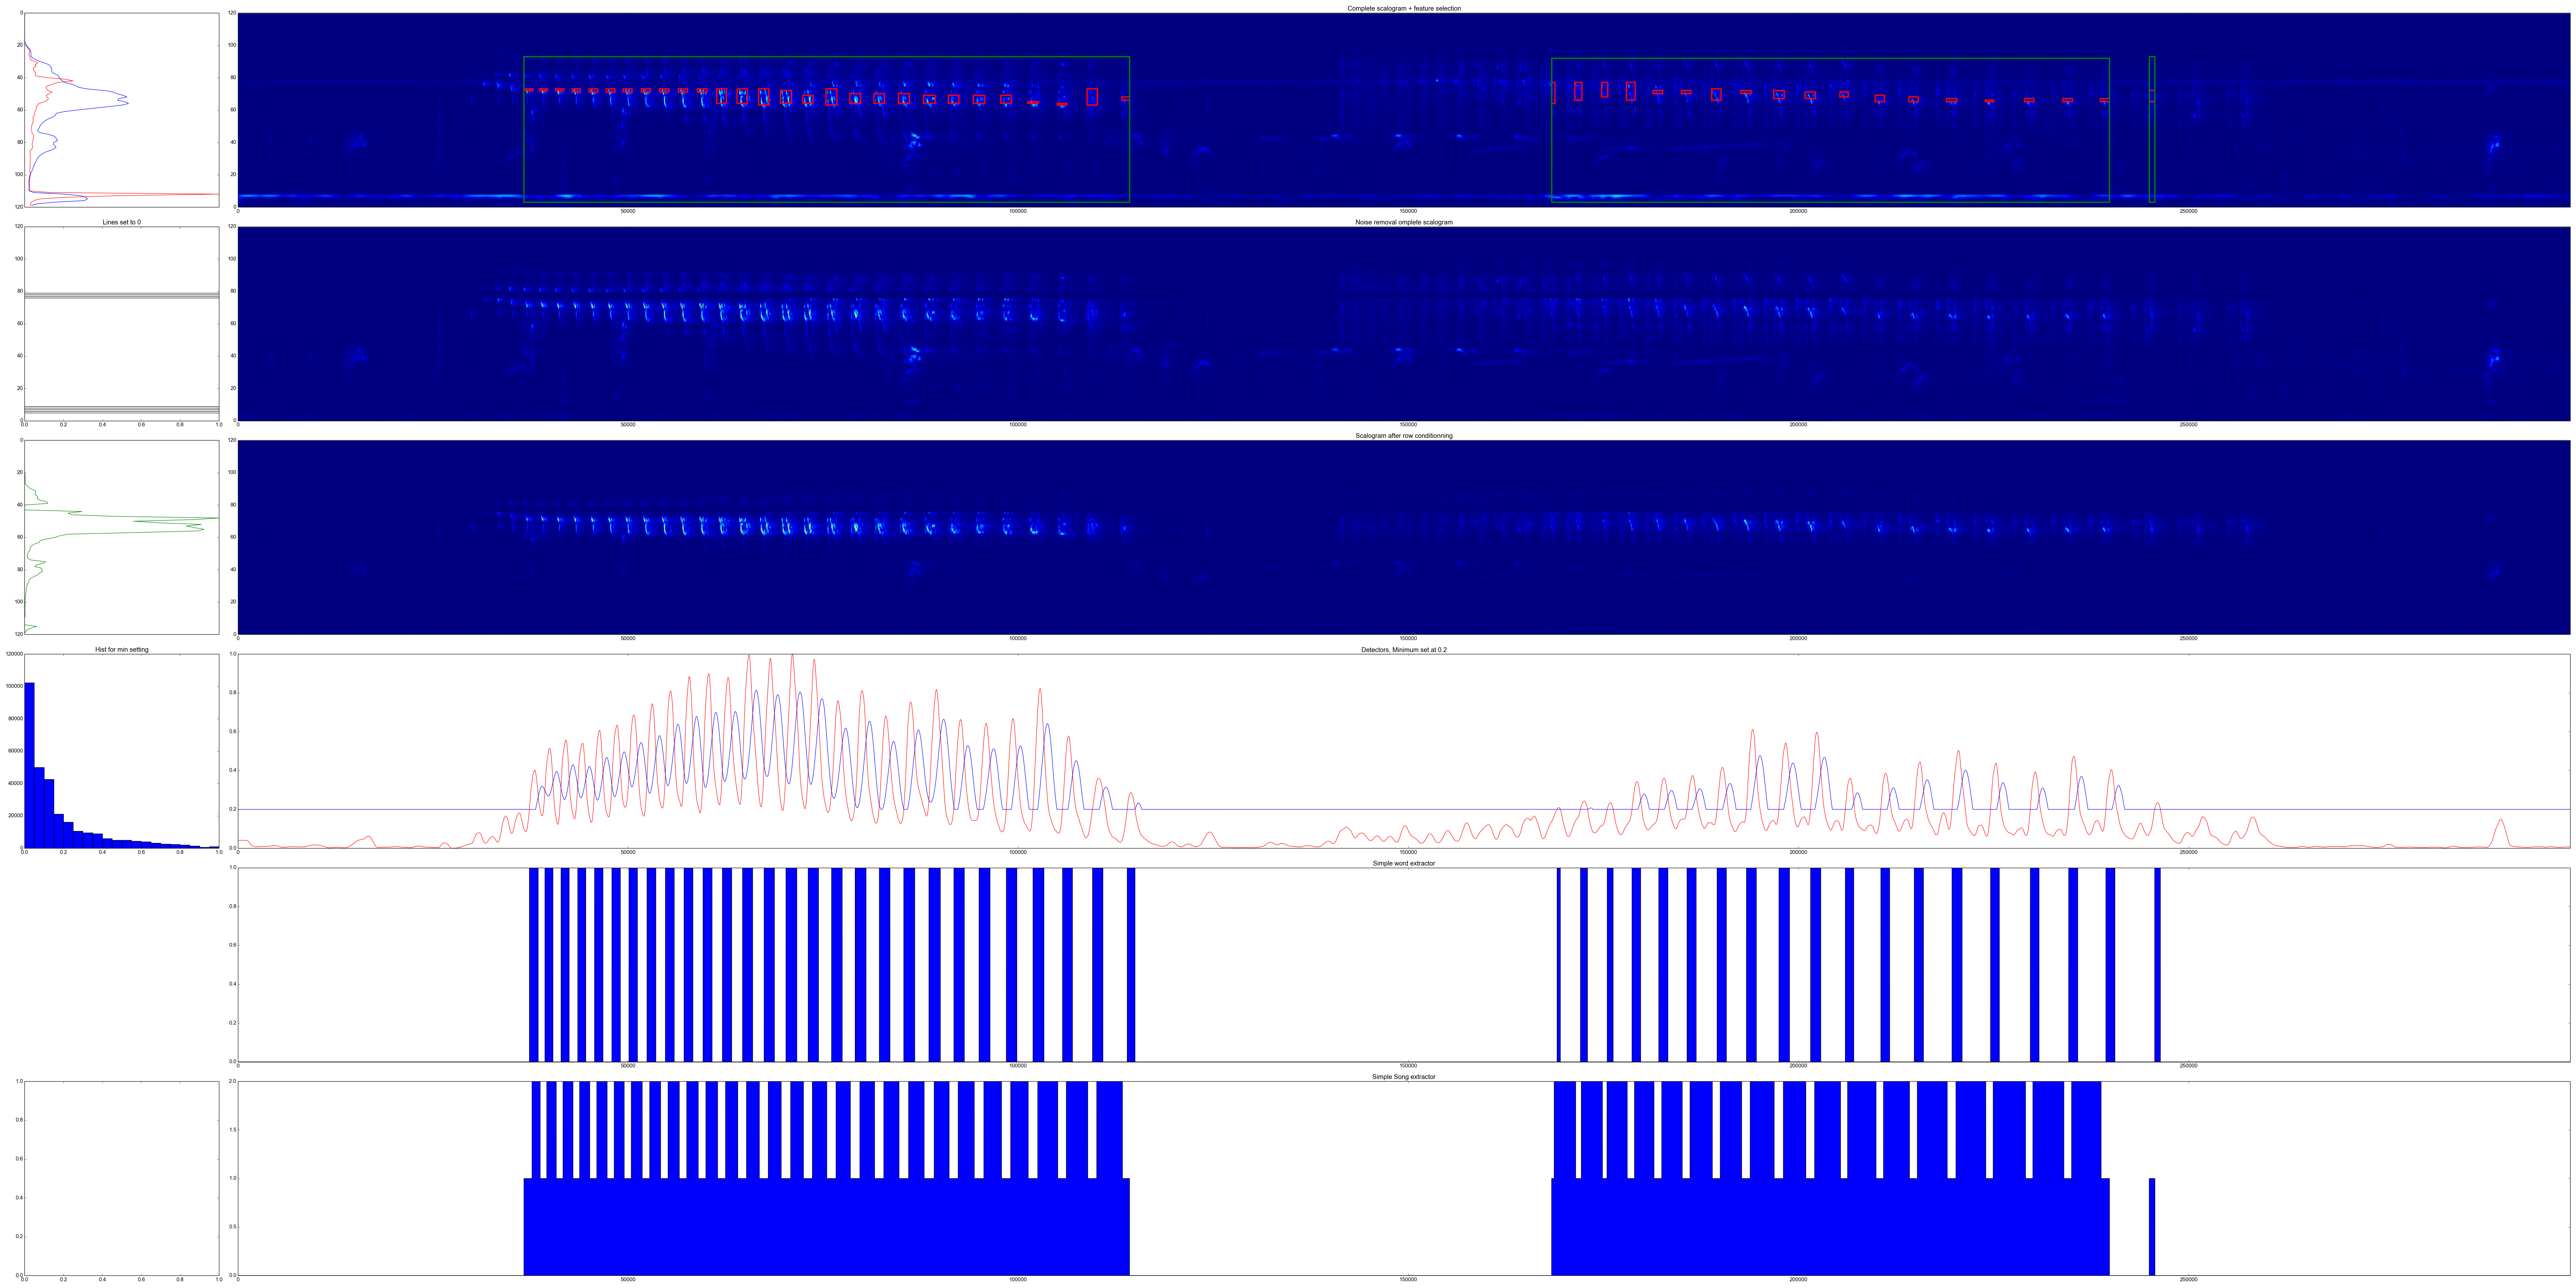
\includegraphics[scale=0.07]{4test.png}\caption{Signal : RN1136.wav with application of the automatic feature extractor, each subplot represents : \ref{LEGENDA} }
\end{center}
\end{figure}


\begin{figure}[H]
\begin{center}
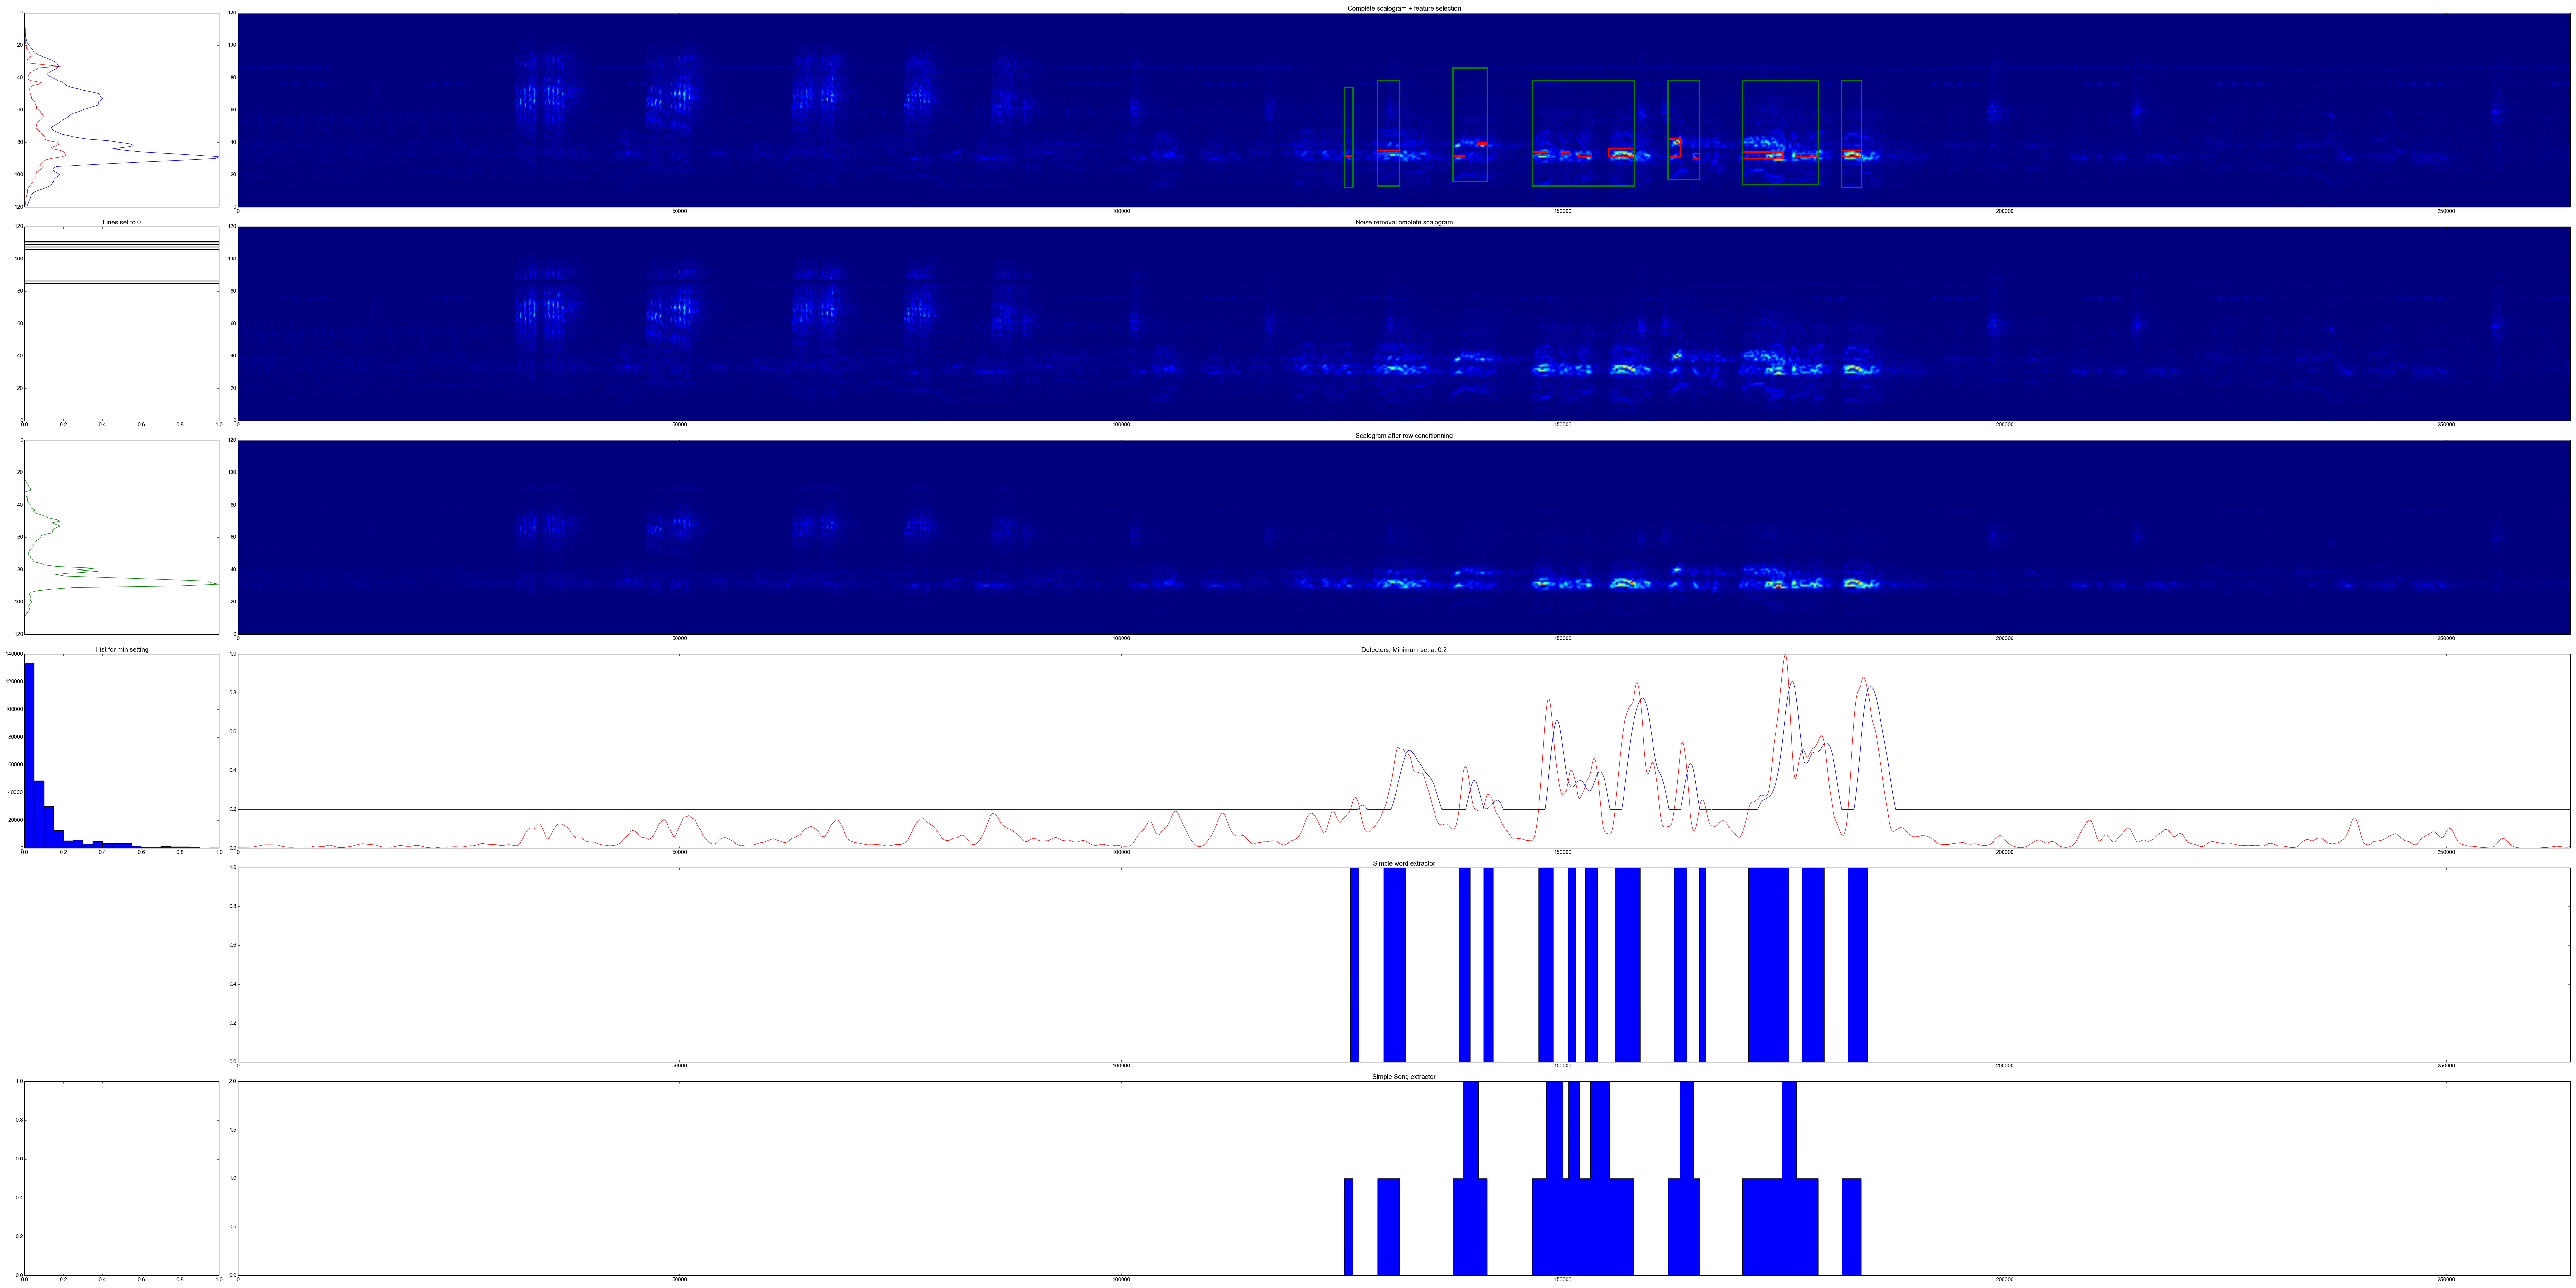
\includegraphics[scale=0.07]{6test.png}\caption{Signal : RN1017.wav with application of the automatic feature extractor, each subplot represents : \ref{LEGENDA} }
\end{center}
\end{figure}


\begin{figure}[H]
\begin{center}
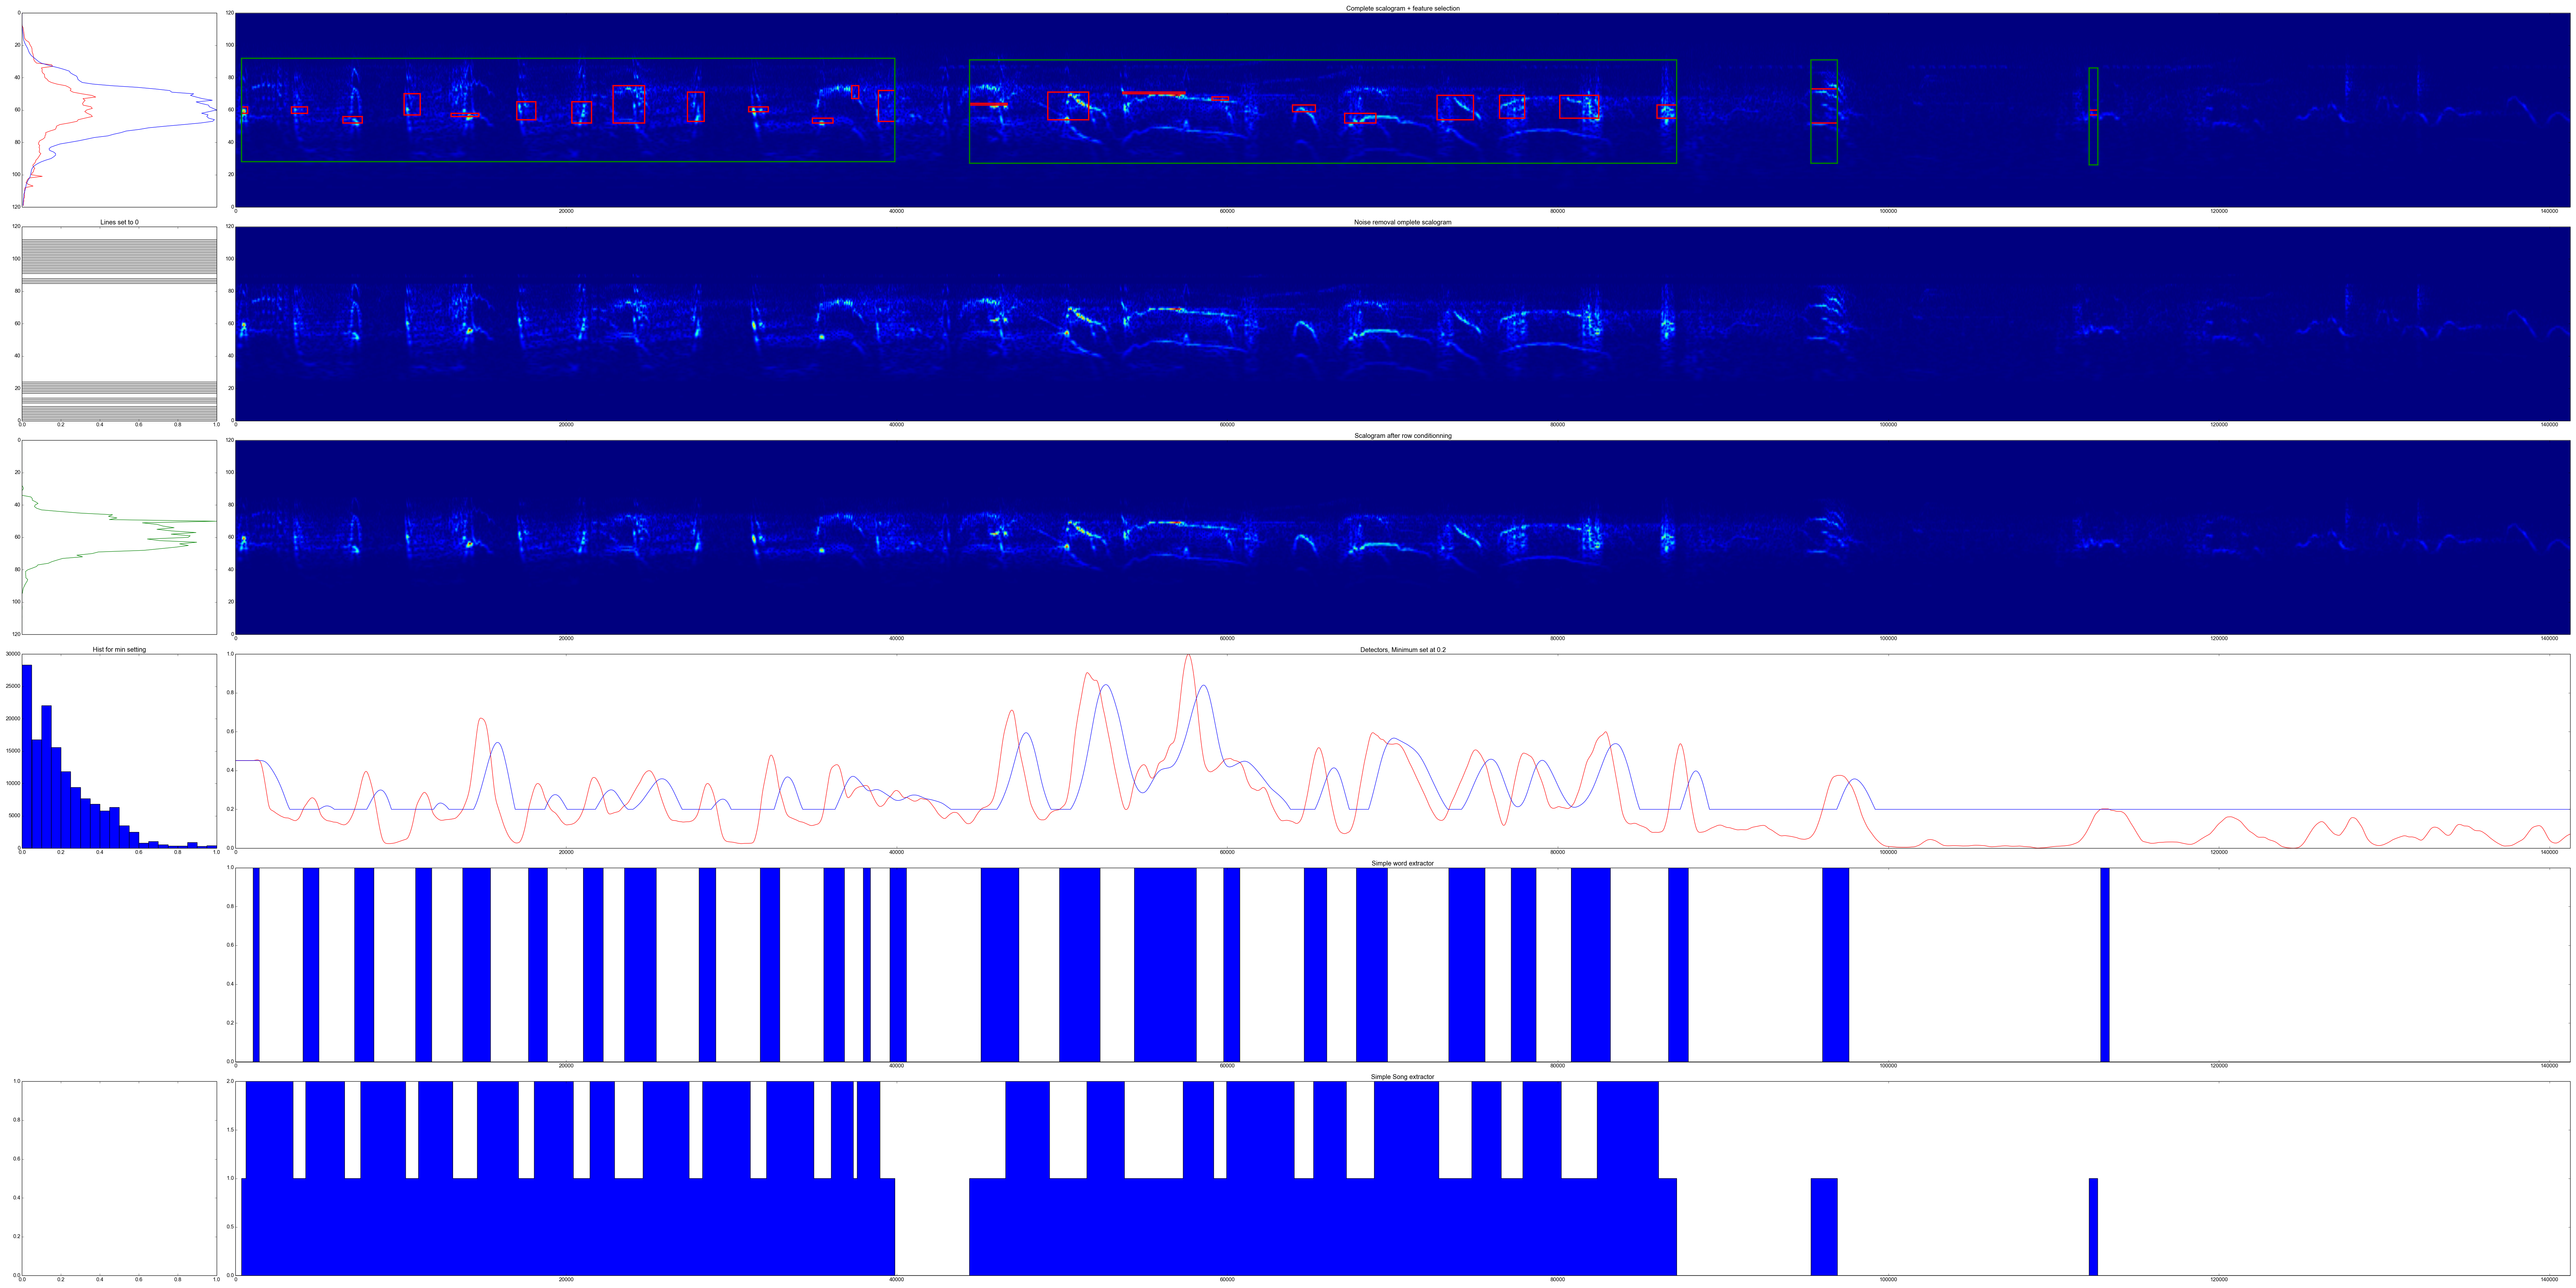
\includegraphics[scale=0.07]{7test.png}\caption{Signal : RN819.wav with application of the automatic feature extractor, each subplot represents : \ref{LEGENDA} }
\end{center}
\end{figure}

\begin{figure}[H]
\begin{center}
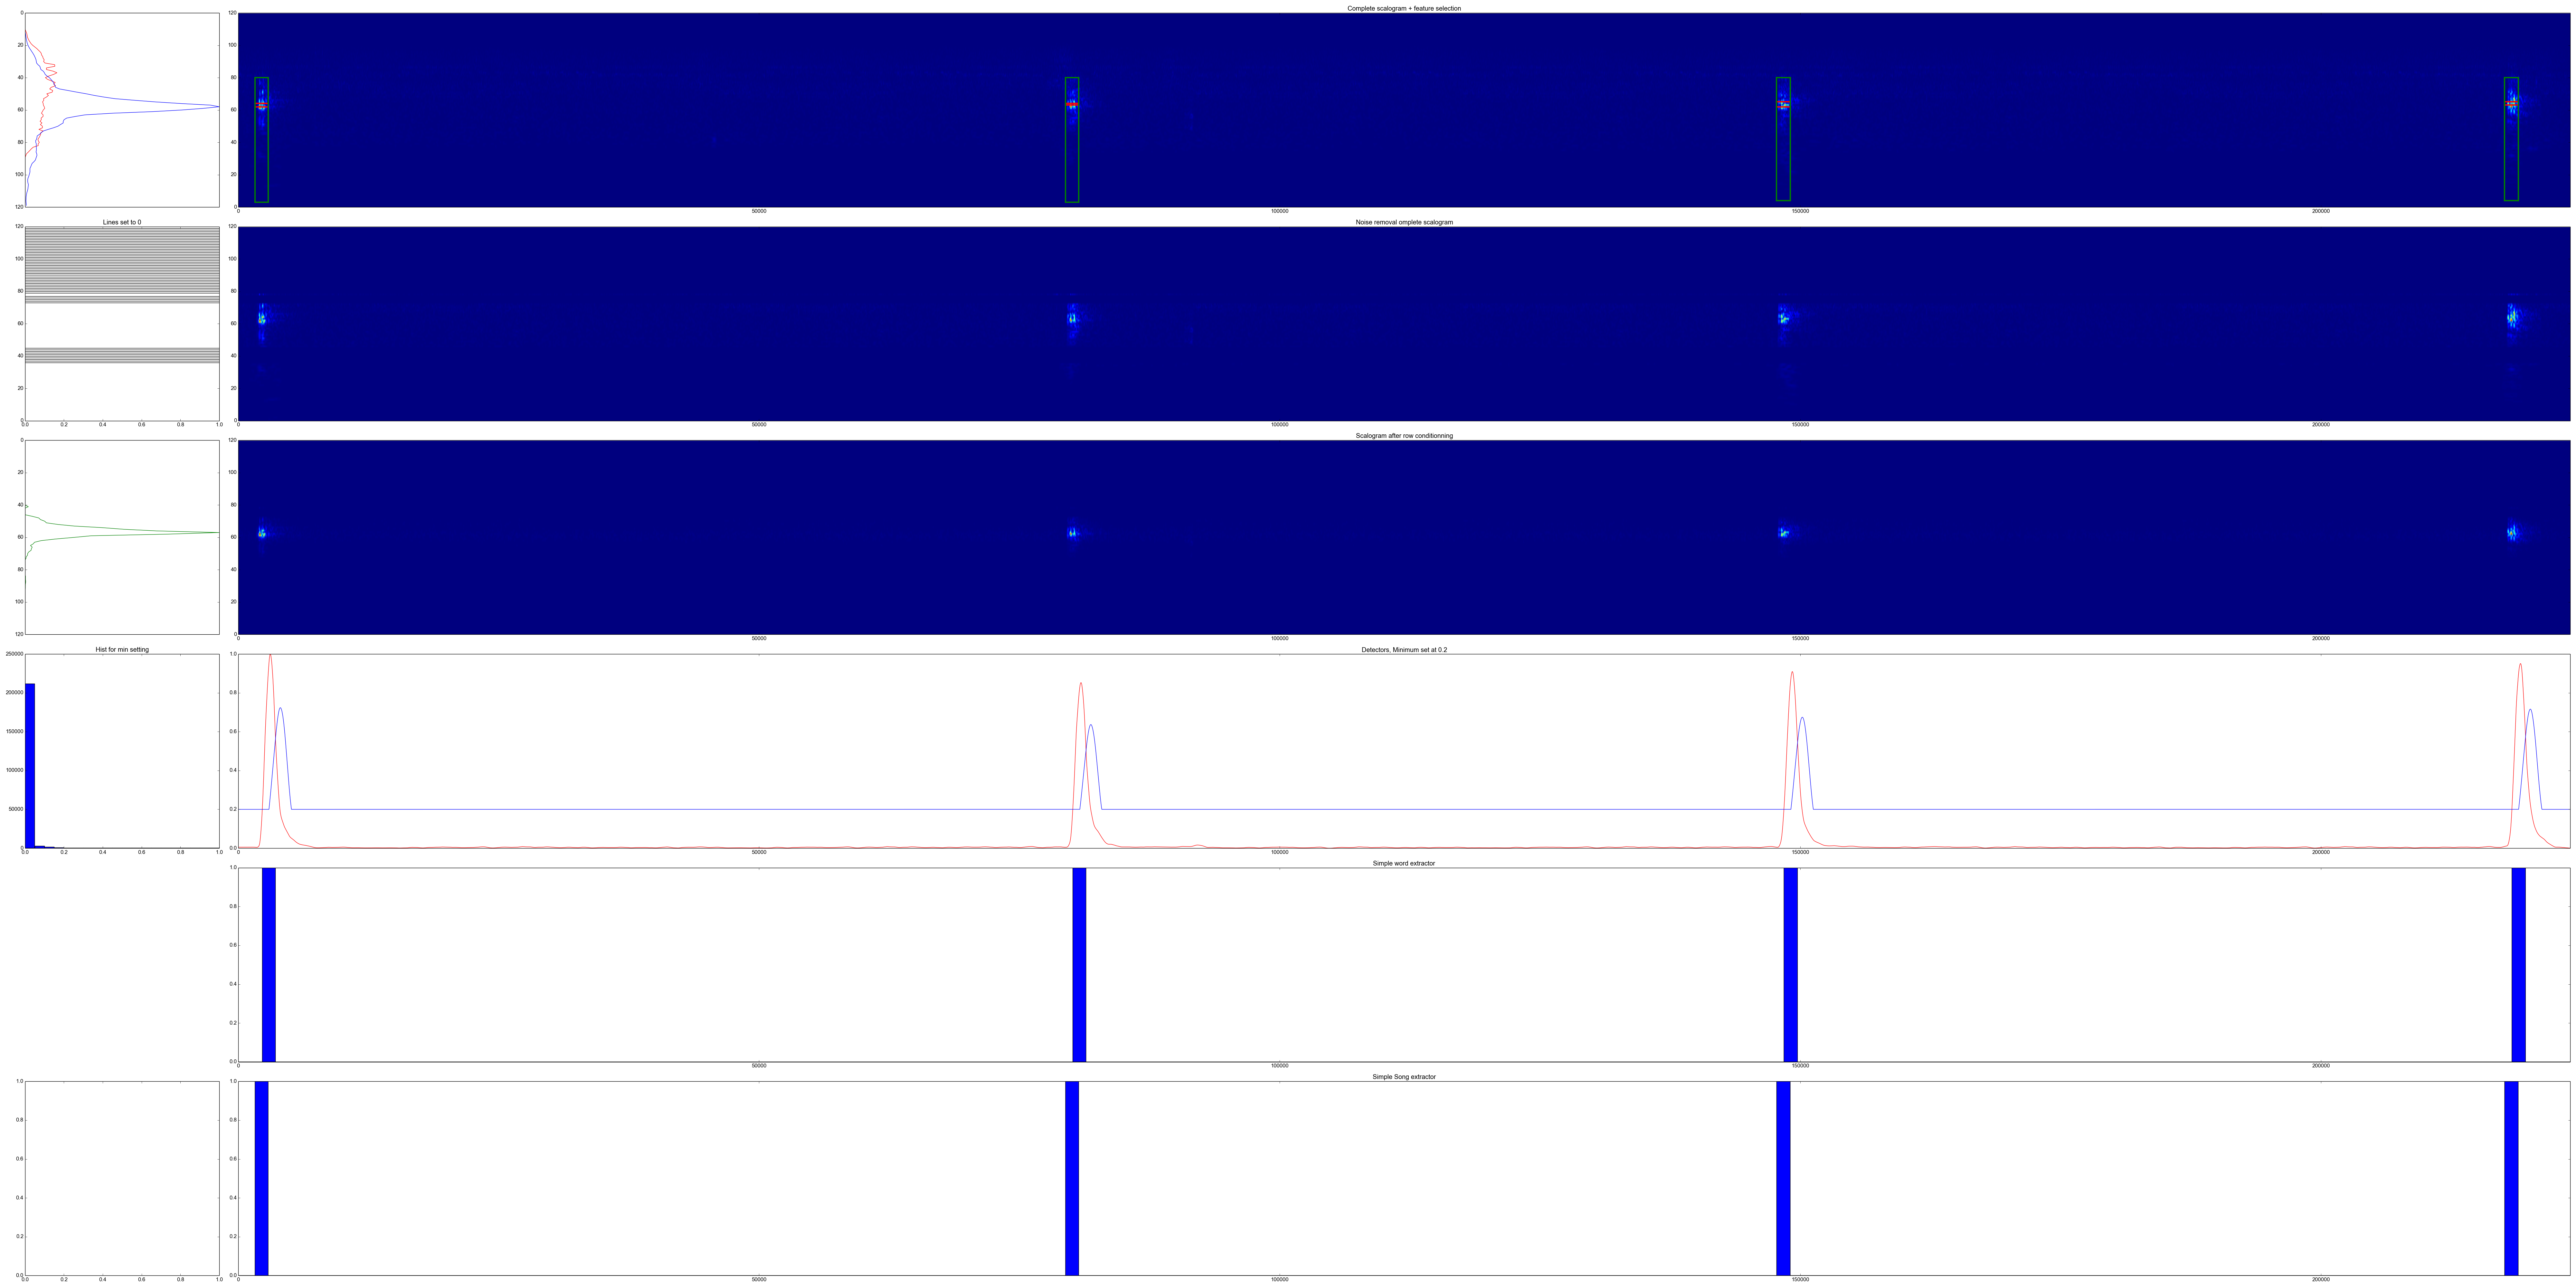
\includegraphics[scale=0.07]{8test.png}\caption{Signal : RN7315.wav with application of the automatic feature extractor, each subplot represents : \ref{LEGENDA} }
\end{center}
\end{figure}

\subsection{Conclusion}
The main encountered problems for this task are now listed and analysed.
\begin{itemize}
\item Intra/Inter-class variance. First of all, when looking at the bird songs in a time-frequency representation (scalogram or spectrogram) the examples from within the same class have a huge intra-class variance. This means that even in this new space, the same class has not always observations that are close from each other. 
\\
On the other hand, when looking at examples from different classes, the difference between the song representation is sometimes really small.
\item Noise/Non bird sounds. The second problem is the presence of other species inside the audio recordings. This is particularly problematic since it is not only white noise (which could be easily treated with denoising techniques) but also biological sounds such as insect, other background birds, forest sounds,...
\item Number of observation. Another huge point to consider is the number of examples per class. It has been seen for years that if the number of examples per class is great (at least few thousands) some techniques such as Convolutionnal Neural Networks provide state-of-the-art solutions. It is able to perform feature extraction through a learning process of the features by the convolution phase (convolution and pooling in cascade). Then dimensionality reduction and classification is done through a Multi-Layer Perceptron. Unfortunately in our case, the learning process won't converge since we sometimes have as small as few examples per class.
\item Number of Classes. With only a few classes, it would be possible to implement a feature extractor as seen previously since there is no need for generalization. However in our case, overfitting on even some classes can really hurt the overall classification performance. For example even though the past feature extractor could perform very well on at most $10$ classes, applying it for the task would not be competitive. 
\item The database. Finally a natural problem which lies in the nature of the task is the public labelling of the audio recordings. This implies that errors can be made and thus we could learn on false labels and learn structures of the wrong classes.
\end{itemize}
\chapter{Classification Algorithms using the Scattering Network}
\section{One Scattering Layer}
\subsection{Architecture}

This first model is based on a one-layer scattering network leading to a decomposition where the time dimension will be suppressed by aggregating the information using the following statistics on the scattering coefficients : mean max and standard deviation.
The scheme is as follow :

\begin{equation}
\begin{matrix}
\text{Raw Signal Input } x(t) \in \mathbb{R}^N \\
\text{ normalization } \rightarrow x(t) \in  [-1,1], 0 \leq t \leq N \\
\downarrow \\
 | x \star \psi_{1,\lambda_1}  |:= U_1(\lambda_1,t)\\
\downarrow \\
U_1 \star \phi_1 := S_1(\lambda_1,t)
\end{matrix}
\end{equation}

Where we have :\\ 
\[
U_1=\left( \begin{matrix}
|x\star \psi_{1,1} | \\
|x\star \psi_{1,2} | \\
... \\
|x\star \psi_{1,|\lambda_1|} |\\
\end{matrix}
\right)
\in \mathbb{R}^{|\lambda_1|\times N_1}
\]

\[
S_1=\left( \begin{matrix}
|x\star \psi_{1,1} | \star \phi_1 \\
|x\star \psi_{1,2} | \star \phi_1  \\
... \\
|x\star \psi_{1,|\lambda_1|} | \star \phi_1 \\
\end{matrix}
\right)
\in \mathbb{R}^{|\lambda_1|\times N_2}
\]

Then we aggregate the time component using basic descriptive statistics (mean, standard deviation, max) leading to the actual feature vector :
\[
\left(
\begin{matrix}
\overline{S_1}\\
\end{matrix}
\right)
:=
\left(
\begin{matrix}
\frac{\sum_{t=1}^{N_2} S_{1}(1,t)}{N_2}\\
\frac{\sum_{t=1}^{N_2} S_{1}(2,t)}{N_2}\\
...\\
\frac{\sum_{t=1}^{N_2} S_{1}(|\lambda_1|,t)}{N_2}\\
\end{matrix}
\right) \in \mathbb{R}^{|\lambda_1|}
\]
\[
\left(
\begin{matrix}
\sigma(S_1)\\
\end{matrix}
\right)
:=
\left(
\begin{matrix}
\sqrt{\frac{\sum_{t=1}^{N_2} \left( S_{1}(1,t)-\overline{S_{1,1}}\right)^2}{N_2}}\\
\sqrt{\frac{\sum_{t=1}^{N_2}\left(S_{1}(2,t)-\overline{S_{1,2}}\right)^2}{N_2}}\\
...\\
\sqrt{\frac{\sum_{t=1}^{N_2}\left(S_{1}(|\lambda_1|,t)-\overline{S_{1,|\lambda_1|}}\right)^2}{N_2}}\\
\end{matrix}
\right) \in \mathbb{R}^{|\lambda_1|}
\]
\[
\left(
\begin{matrix}
\max_t(S_1)
\end{matrix}
\right)
:=
\left(
\begin{matrix}
\max_{t=1,...,N_2}(S_{1}(1,t))\\
\max_{t=1,...,N_2}(S_{1}(2,t))\\
...\\
\max_{t=1,...,N_2}(S_{1}(| \lambda_1|,t))\\
\end{matrix}
\right) \in \mathbb{R}^{|\lambda_1|}
\]
This choice comes from the fact that the time component contains informations about the interesting (and most likely discriminative) behaviours of the bird songs. However, the location in time of these features is not at all required to classify a signal. This is why time-invariance is such an important property.
\\
The degrees of freedom of the model are : 
\begin{itemize}
\item $T$
\item $Q$
\item $J$
\item $h_1$
\end{itemize}
 with $h_1$ being the number of hidden neurons in the classifier.
The parameters $Q$ and $J$ are chosen a priori knowing the communication behaviours of birds. Thus, the parameters $T$ and $h_1$  will have to be selected by optimizing the classification accuracy. A common method to select a coefficient is cross-validation. We basically compute the accuracy of the trained model for each value and then keep the best one. Obviously, the values to be tested can be a priori reduced or influenced using some probabilistic methods for example.

\subsection{Cross-validation : T}
The coefficients determining the filter banks are $T, Q, J$. By knowing the biological specifications of birds we can determine almost surely $Q$ and $J$. The parameter $T$ on the other hand has to be cross-validated since it is not easy a priori to determine the amount of time invariance we want to introduce in the first layer of the scattering network. In fact, having a large $T$ can reduce the variance but this can hide some discriminative informations (the structure of fast bird calls for example) and so can make two different birds have the same scattering representation. On the contrary, having a too small $T$ will leave us with a huge variance which will be mainly made of noise (thus non informative). Having the chance to be in a supervised learning task, applying cross-validation on this parameter is the best way to maximize our prediction accuracy.\\
Let's look at the prediction accuracy for given values of $T$ :

\begin{figure}[H]
\begin{center}
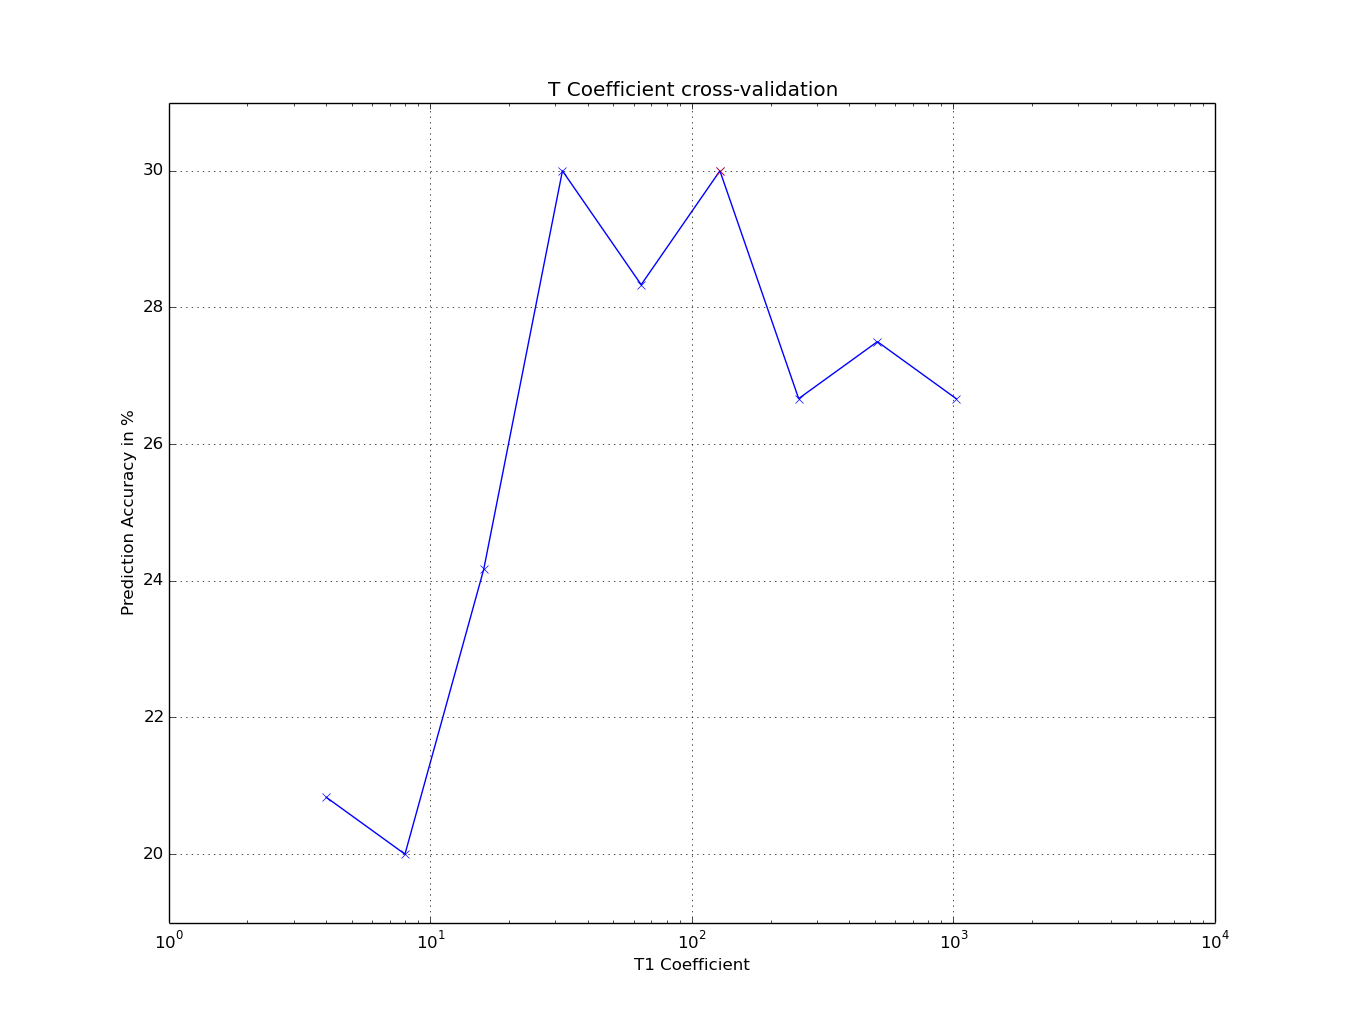
\includegraphics[scale=0.25]{T_S0.png}\caption{x-axis in log scale since we use power of $2$}\label{figure4}
\end{center}
\end{figure}
Having two identical results, we will take the greater $T$ allowing reduced variance (without loss of information according to the prediction accuracy). By doing so we also reduce the time dimension of the scattering transformation leading to faster computation and less memory requirements. 

\subsection{Cross-validation : Features}
Not only the representation has to be tuned but the features computed from it have to be chosen too. At a first shot we might say that the most simple (but  informative) statistics are the mean, maximum and standard deviation. More complicated features could be computed from the scattering coefficients such as the Discrete Cosine Transform, allowing time invariance while keeping informations on the structure of the scattering coefficients for example.

Even with these $3$ simple statistics, we can see that the features can be correlated. Let's look at a plot of each statistics for the first $25$ classes. Each column is a feature vector made of $80$ coefficients (the statistics for the $80$ lines of the scattering). Since we have $15$ examples by class we end up with a matrix feature of size $80\times 15$ for each class.
\begin{figure}[H]
\begin{center}
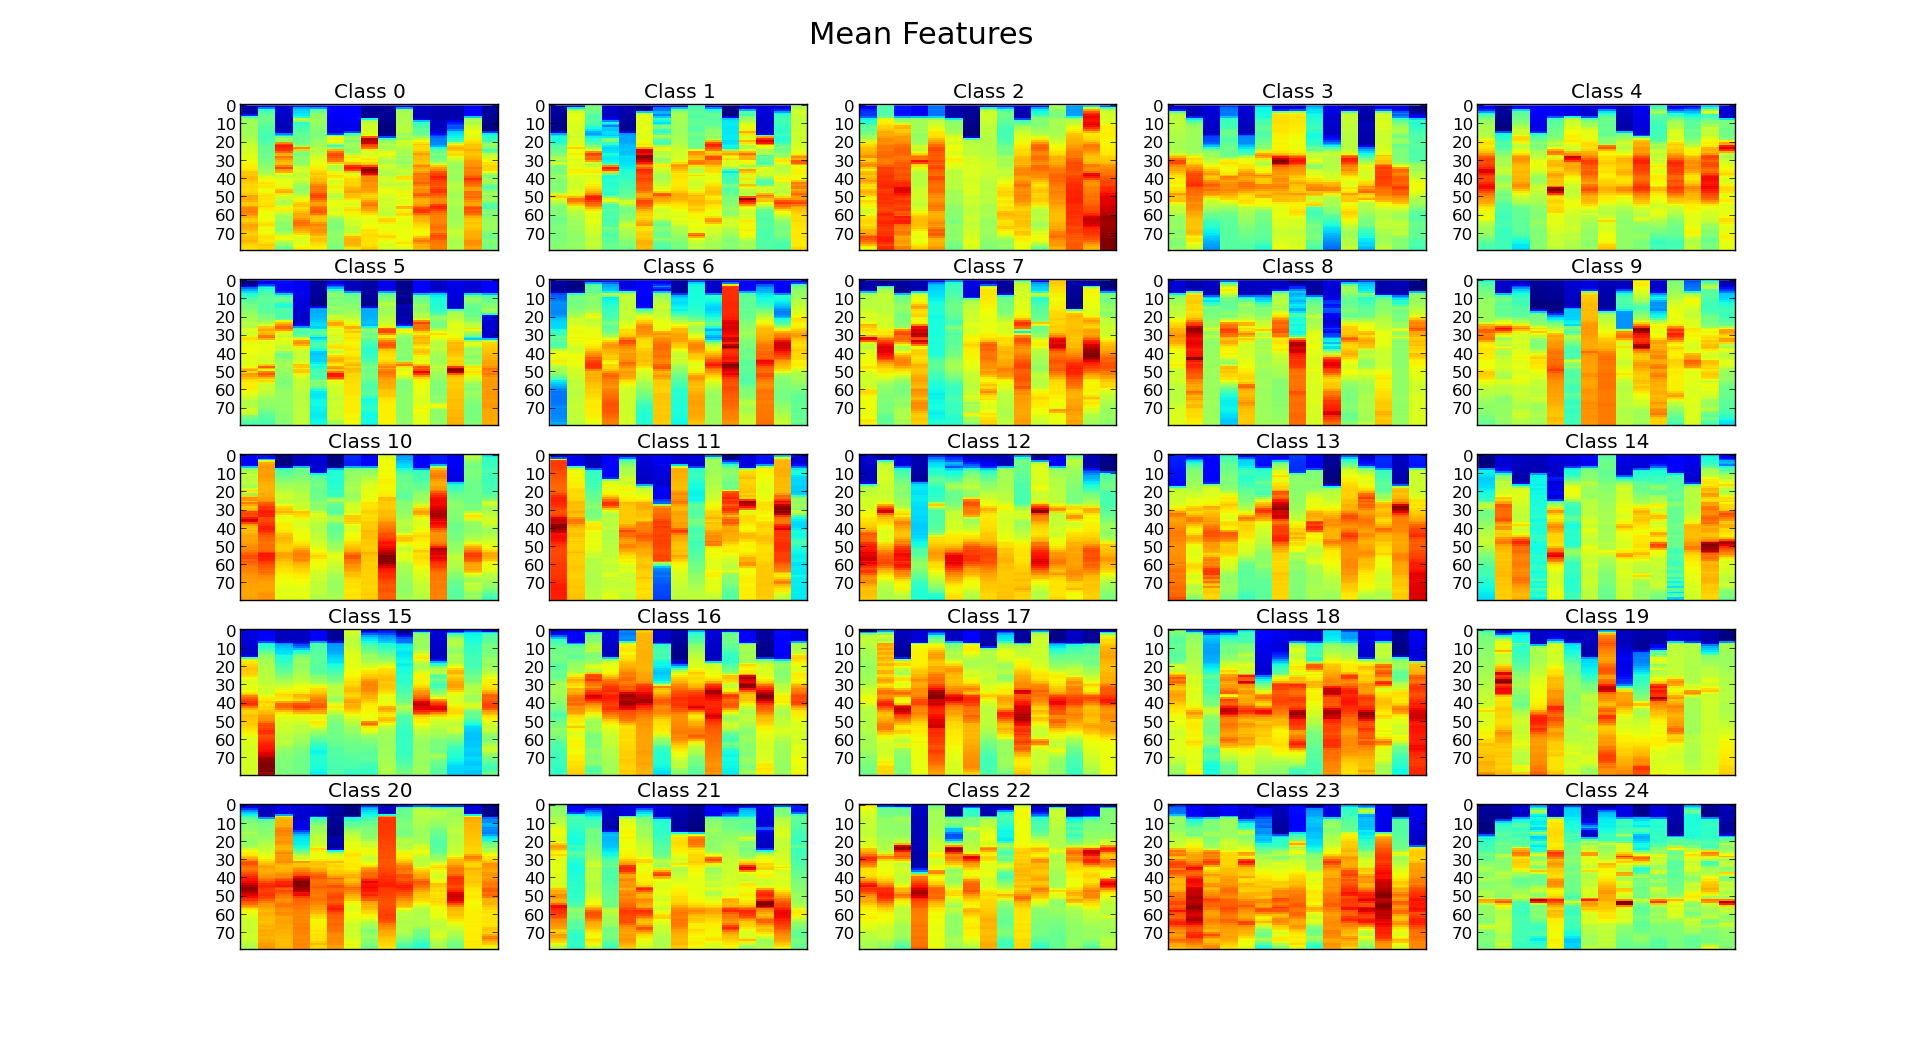
\includegraphics[scale=0.25]{mean_S0.png}\caption{The 80 mean features for the first 25 classes.}\label{meanfeatures}
\end{center}
\end{figure}

\begin{figure}[H]
\begin{center}
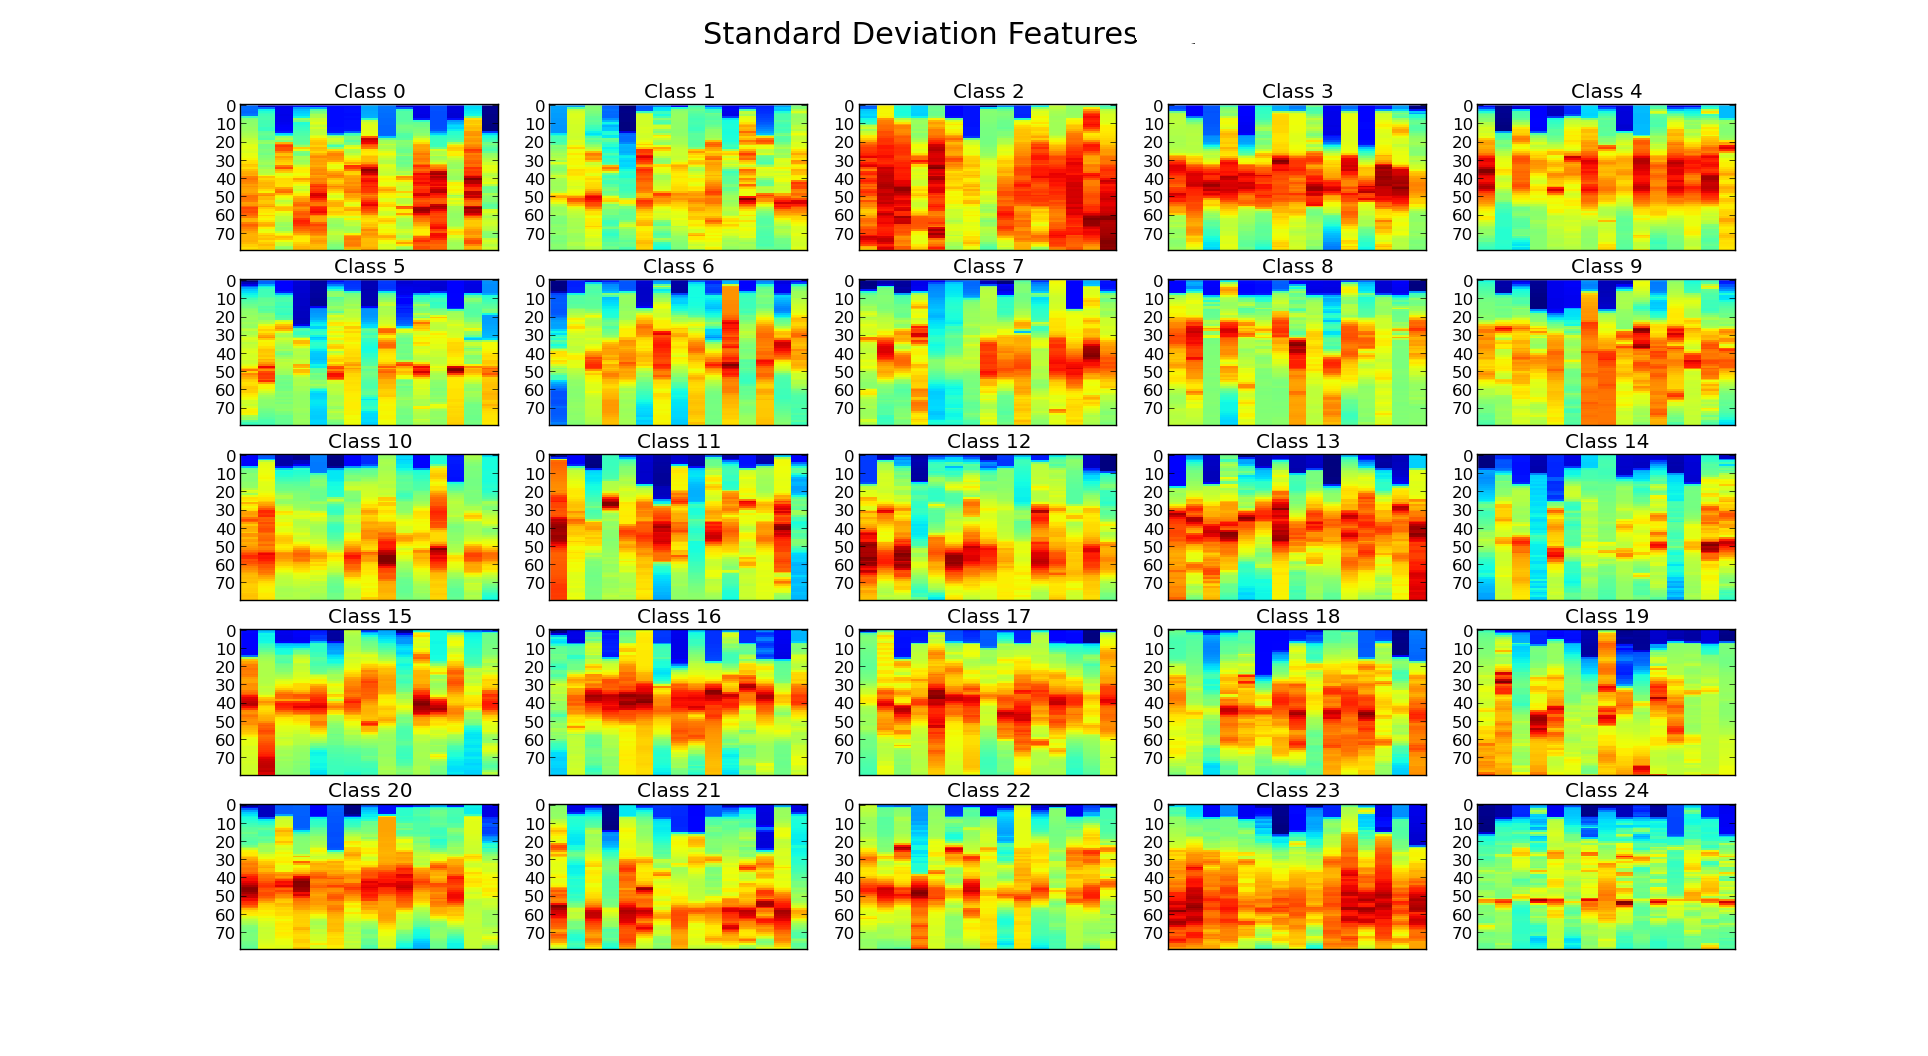
\includegraphics[scale=0.25]{std_S0.png}\caption{The 80 standard deviation features for the first 25 classes.}\label{stdfeatures}
\end{center}
\end{figure}

\begin{figure}[H]
\begin{center}
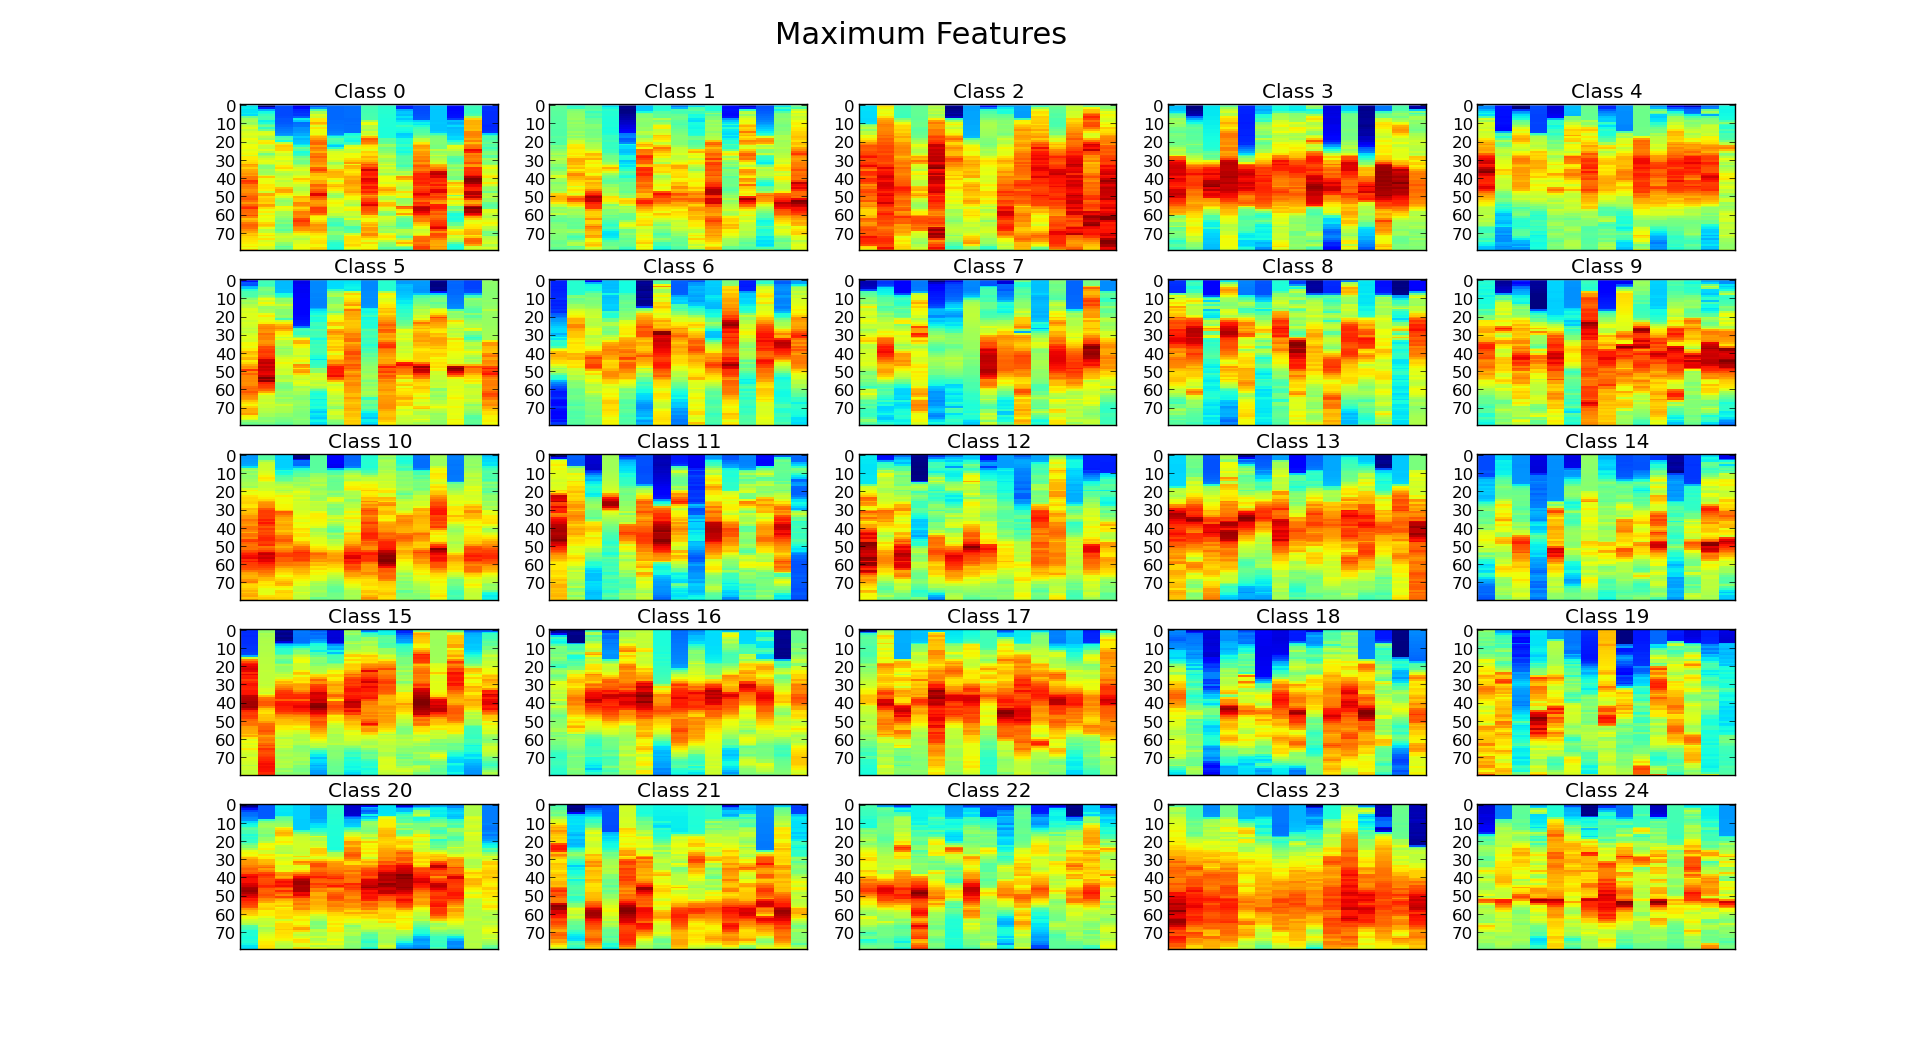
\includegraphics[scale=0.25]{maximum_S0.png}\caption{The 80 maximum features for the first 25 classes.}\label{maxfeatures}
\end{center}
\end{figure}
We can see that for some examples, the maximum feature seem more reliable. The standard deviation also seems to be more robust than the mean in any cases.
Let's look at the correlations between these features :
\begin{figure}[H]
\begin{center}
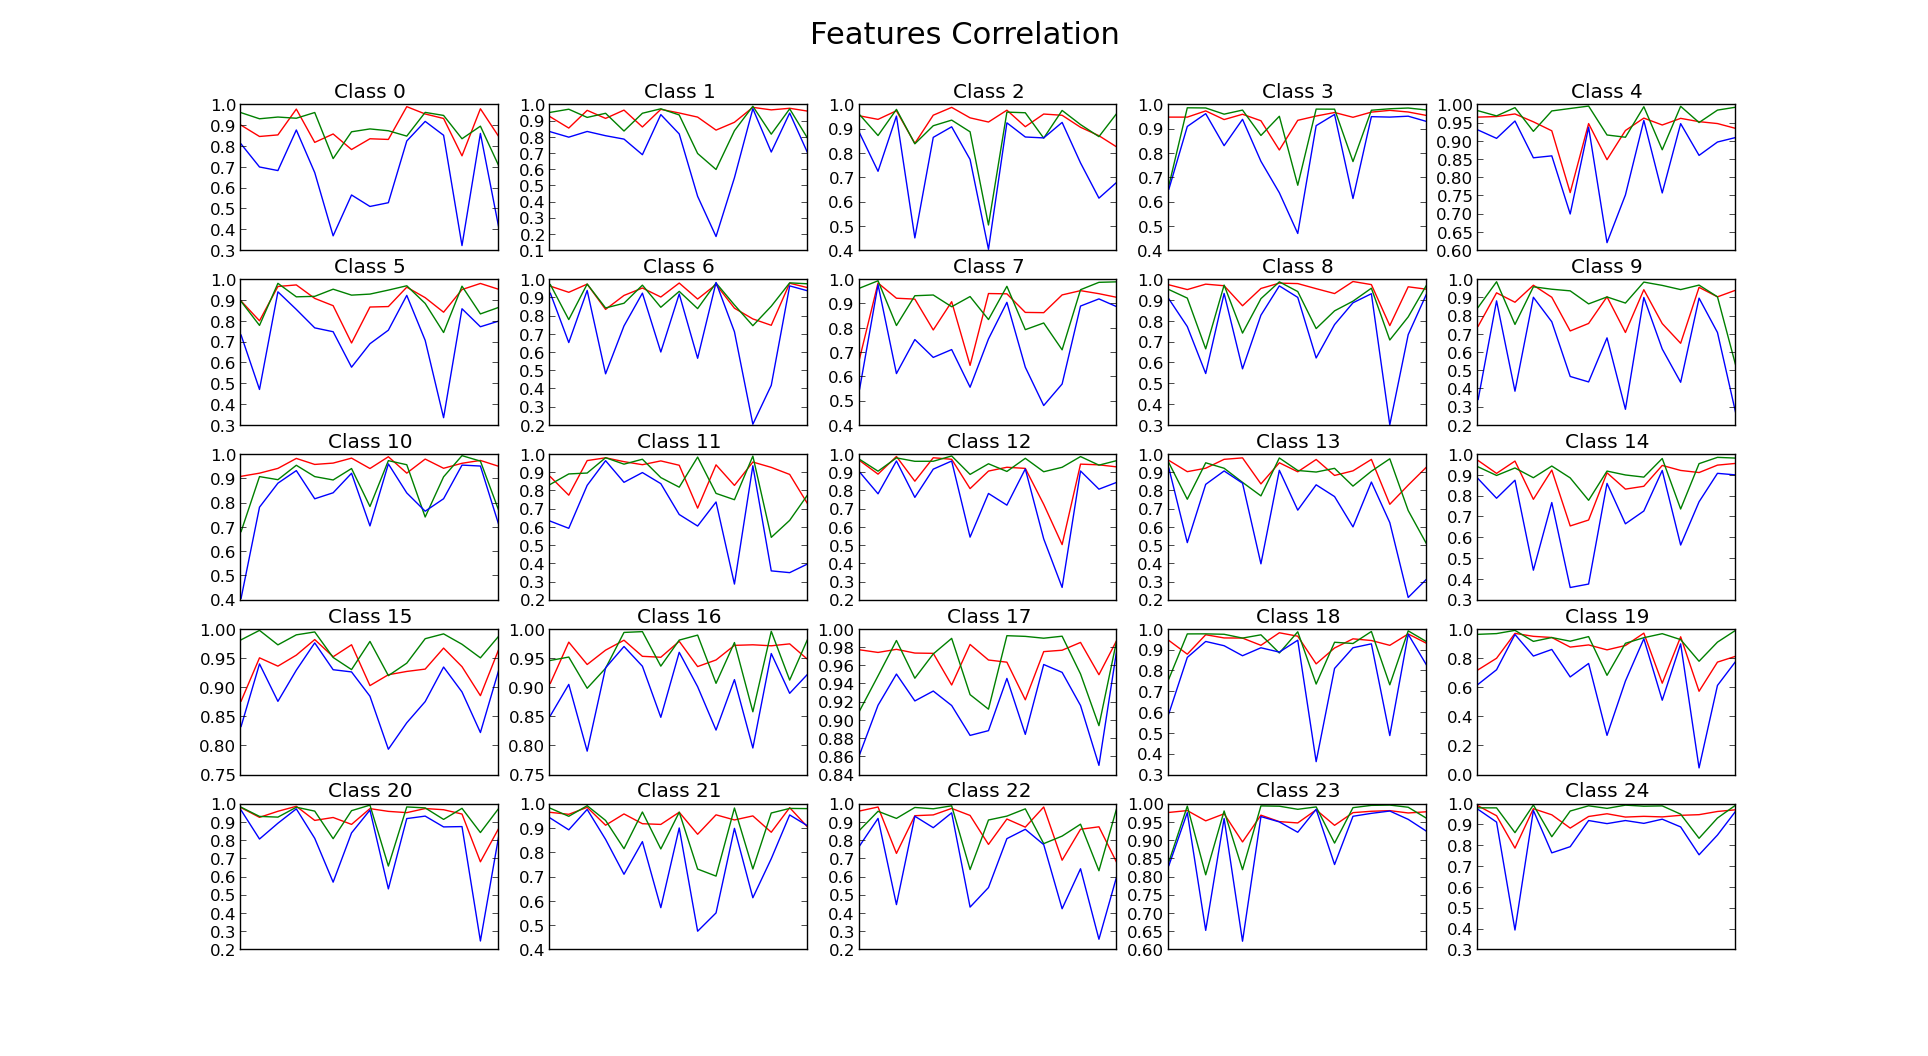
\includegraphics[scale=0.25]{corr_S0.png}\caption{The correlation coefficient : red = STDvsMAX green = STDvsMEAN blue = MAXvsMEAN.}\label{featurescorrelation}
\end{center}
\end{figure}
We can see that STDvsMEAN and MAXvsMEAN are not as correlated as STDvsMAX. We now have to know if they are less correlated because they are complementary or because one is more robust than the other.
Let's now look at the prediction accuracy for each kind of feature combination :
\begin{figure}[H]
\begin{center}
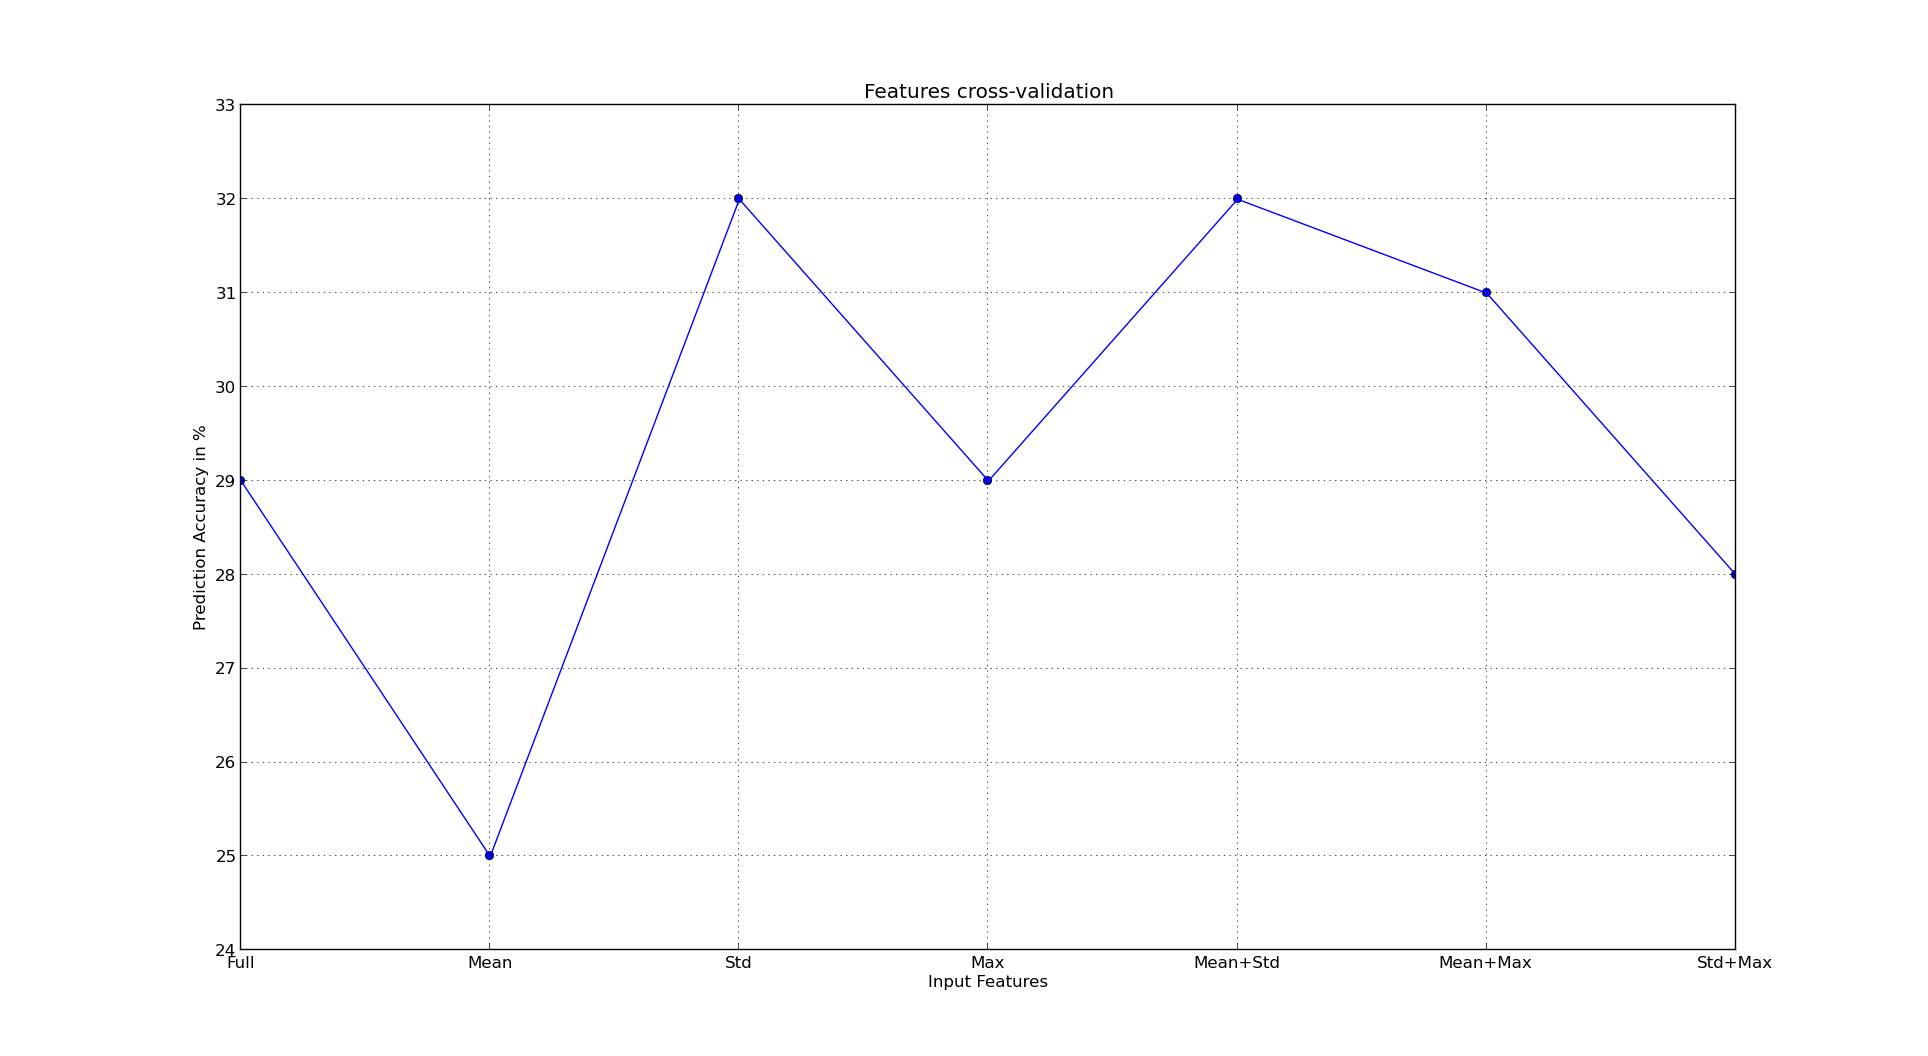
\includegraphics[scale=0.2]{features_cross_S0.png}\caption{Cross-validation of the input features}\label{figure4}
\end{center}
\end{figure}
We can see that only the standard deviation features provide the best information, we will then keep this configuration meaning that with only $80$ coefficients we are able to reach the best accuracy for the given architecture.
\subsection{Cross-validation : Neurons}
Finally, the classifier itself needs some fine-tuning. The main parameter is the number of hidden neurons for the hidden layer of our two-layer perceptron.
Let's look at the leverage of this parameter on the prediction accuracy :
\begin{figure}[H]
\begin{center}
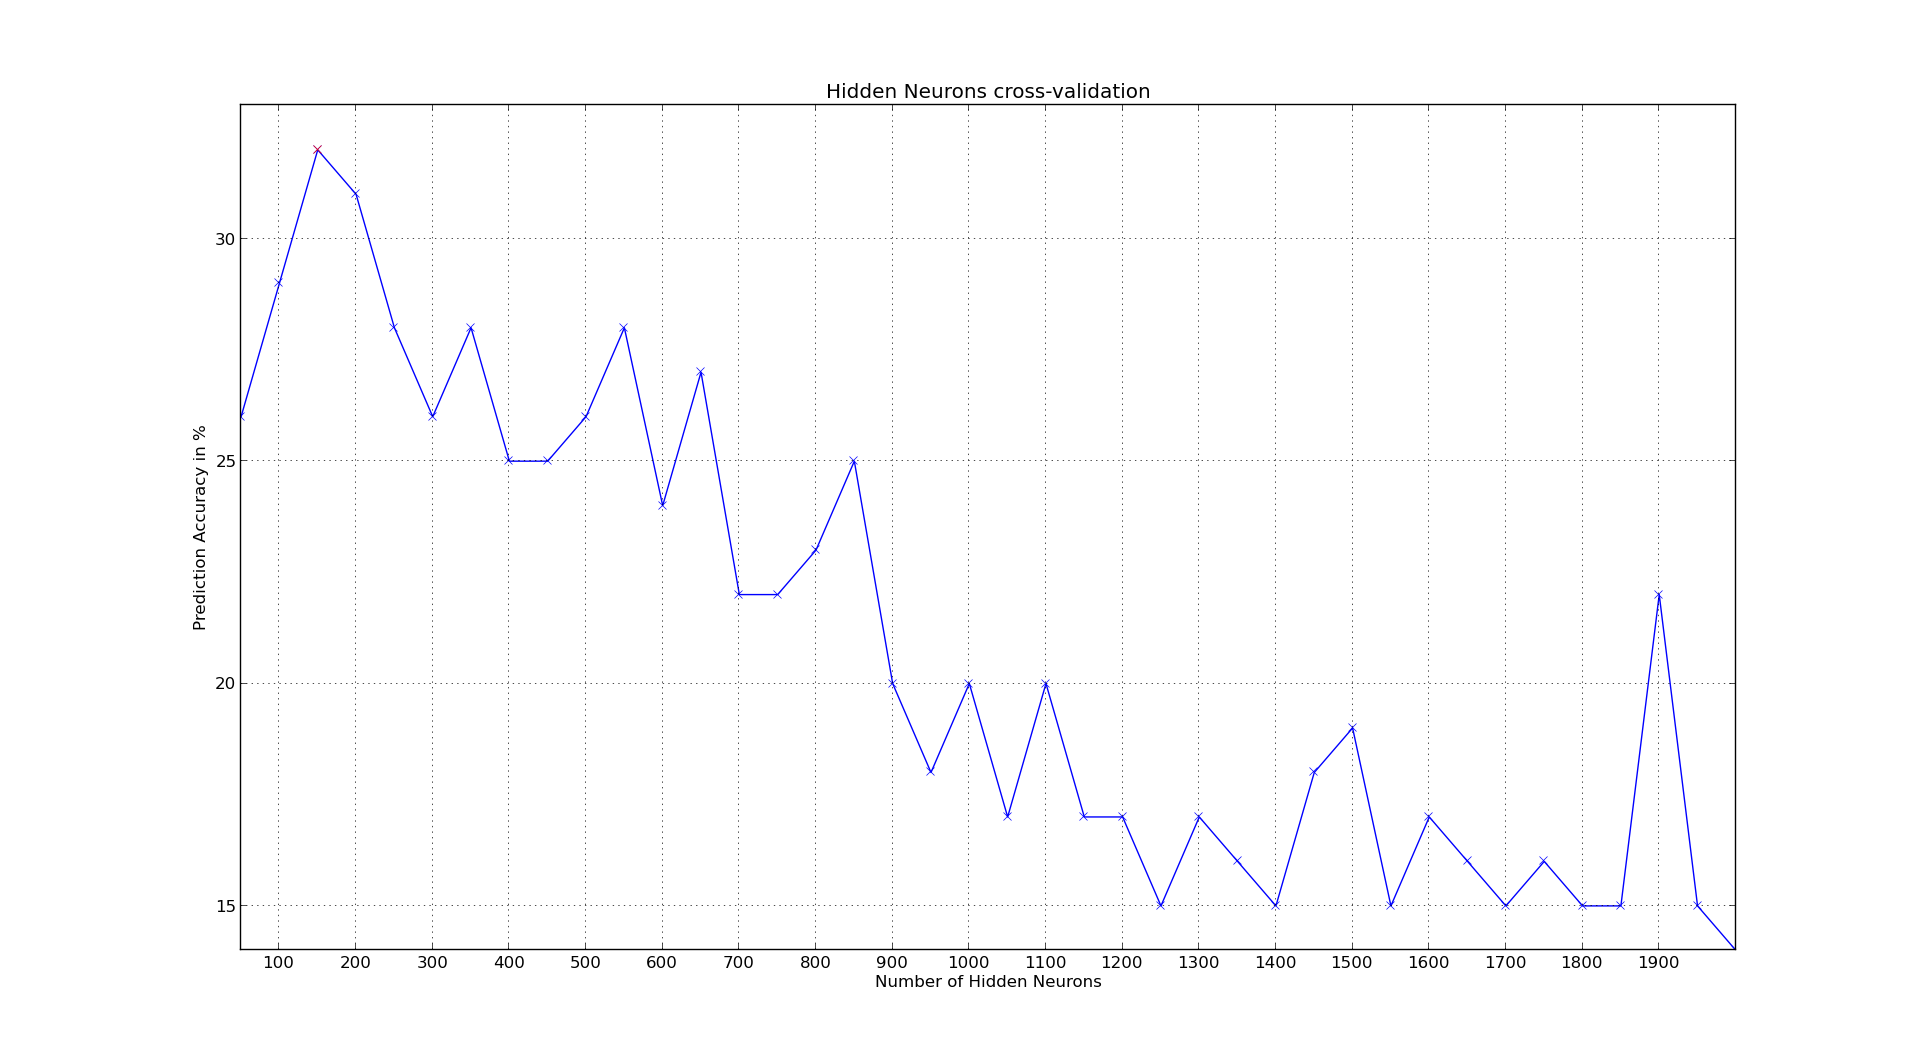
\includegraphics[scale=0.20]{hidden_S0.png}\caption{Cross-validation of Hidden neurons : max 32\%}\label{figure4}
\end{center}
\end{figure}
We now have our (close to the) best configuration from the scattering network parameters to the classifier. Note that the learning rate, the momentum, the L1/L2 norms conditions are left with the default "rule-of-thumb" value.
\subsection{Results Summary and Discussions}
After every step of the cross-validation process we  end up with a classification accuracy of $32\%$ for $45$ classes and with a feature vector of size $80$. It is clear that we lack information about the structure of the scattering coefficients. With the standard deviation we don't have access to information such as the repartition of the coefficients (rithmicity), the transition probabilities,...
One way to capture more information without having to use more complicated statistics is to use a second scattering layer which will actually capture some of this missing information by its underlying (more complex) structure.
\section{Two Scattering Layers}
\subsection{Architecture}
The architecture now is an extension of the last one. We compute a first layer which is then used to computed a second scattering layer to then apply the features computation and the classification algorithm.\\
Let's look at the scheme : 
\begin{equation}
\begin{array}{c c c}
\text{Raw Signal Input } x(t)\in \mathbb{R}^N & & \\
\text{ normalization } \rightarrow x(t) \in  [-1,1], 0\leq t\leq N & & \\
\downarrow & &\\
 | x \star \psi_{1,\lambda_1}  |:= U_1(\lambda_1,t) \in \mathbb{R}^{|\lambda_1| \times N_1} & \rightarrow & |U_1 \star \psi _{2,\lambda_2}| := U_2(\lambda_1,\lambda_2,t) \in \mathbb{R}^{|\lambda_1|*|\lambda_2| \times N_3} \\
\downarrow & & \downarrow \\
U_1 \star \phi_1 := S_1(\lambda_1,t)\in \mathbb{R}^{|\lambda_1| \times N_2} & &U_2 \star \phi_2 := S_2(\lambda_1,\lambda_2,t)\in \mathbb{R}^{|\lambda_1|*|\lambda_2| \times N_4} 
\end{array}
\end{equation}
Where we have :\\ 
\[
U_1=\left( \begin{matrix}
|x\star \psi_{1,1} | \\
|x\star \psi_{1,2} | \\
... \\
|x\star \psi_{1,|\lambda_1|} |\\
\end{matrix}
\right)
\in \mathbb{R}^{|\lambda_1|\times N_1}
\]

\[
S_1=\left( \begin{matrix}
|x\star \psi_{1,1} | \star \phi_1 \\
|x\star \psi_{1,2} | \star \phi_1  \\
... \\
|x\star \psi_{1,|\lambda_1|} | \star \phi_1 \\
\end{matrix}
\right)
\in \mathbb{R}^{|\lambda_1|\times N_2}
\]

\[
U_2=\left( \begin{matrix}
||x\star \psi_{1,1} | \star \psi_{2,1} |\\
||x\star \psi_{1,2} | \star \psi_{2,1} |\\
... \\
||x\star \psi_{1,|\lambda_1|} |\star \psi_{2,1}|\\
||x\star \psi_{1,1} | \star \psi_{2,2} |\\
||x\star \psi_{1,2} | \star \psi_{2,2} |\\
... \\
||x\star \psi_{1,|\lambda_1|} |\star \psi_{2,2}|\\
...\\
||x\star \psi_{1,1} | \star \psi_{2,| \lambda_2|} |\\
||x\star \psi_{1,2} | \star \psi_{2,| \lambda_2|} |\\
... \\
||x\star \psi_{1,|\lambda_1|} |\star \psi_{2,| \lambda_2|}|
\end{matrix}
\right)
\in \mathbb{R}^{|\lambda_1|* | \lambda_2 |\times N_3}
\]

\[
S_2=\left( \begin{matrix}
||x\star \psi_{1,1} | \star \psi_{2,1} |\star \phi_2 \\
||x\star \psi_{1,2} | \star \psi_{2,1} |\star\phi_2 \\
... \\
||x\star \psi_{1,|\lambda_1|} |\star \psi_{2,1}|\star\phi_2 \\
||x\star \psi_{1,1} | \star \psi_{2,2} |\star\phi_2 \\
||x\star \psi_{1,2} | \star \psi_{2,2} |\star\phi_2 \\
... \\
||x\star \psi_{1,|\lambda_1|} |\star \psi_{2,2}|\star\phi_2 \\
...\\
||x\star \psi_{1,1} | \star \psi_{2,| \lambda_2|} |\star\phi_2 \\
||x\star \psi_{1,2} | \star \psi_{2,| \lambda_2|} |\star\phi_2 \\
... \\
||x\star \psi_{1,|\lambda_1|} |\star \psi_{2,| \lambda_2|}|\star\phi_2 
\end{matrix}
\right)
\in \mathbb{R}^{|\lambda_1|* | \lambda_2 |\times N_4}
\]

We now compute the statistics on $S_2$ leading to a feature vector of greater dimension. We will also explore the case where we concatenate the feature of $S_1$ and $S_2$.
\\
The degrees of freedom are now : $T_1$, $Q_1$, $J_1$,$T_2$, $Q_2$, $J_2$, $h_1$ with $h_1$ being the number of hidden neurons in the classifier.
The parameters $T_1$, $Q_1$, $J_1$ are chosen to be the optimized coefficients of the one-layer case. The parameters $Q_2$ and $J_2$ are chosen a priori thus we are left with $T_2$ and $h_1$. In fact the number of hidden neurons has to be optimized again since the input features won't be of the same structure (dimension and underlying relations). Once again these parameters will be optimized through cross-validation.

\subsection{Cross-validation : $T_2$}
The first parameter to cross-validate is the $T_2$ coefficient which defines along $Q_2$ and $J_2$ the second $\psi$ filter bank.
\begin{figure}[H]
\begin{center}
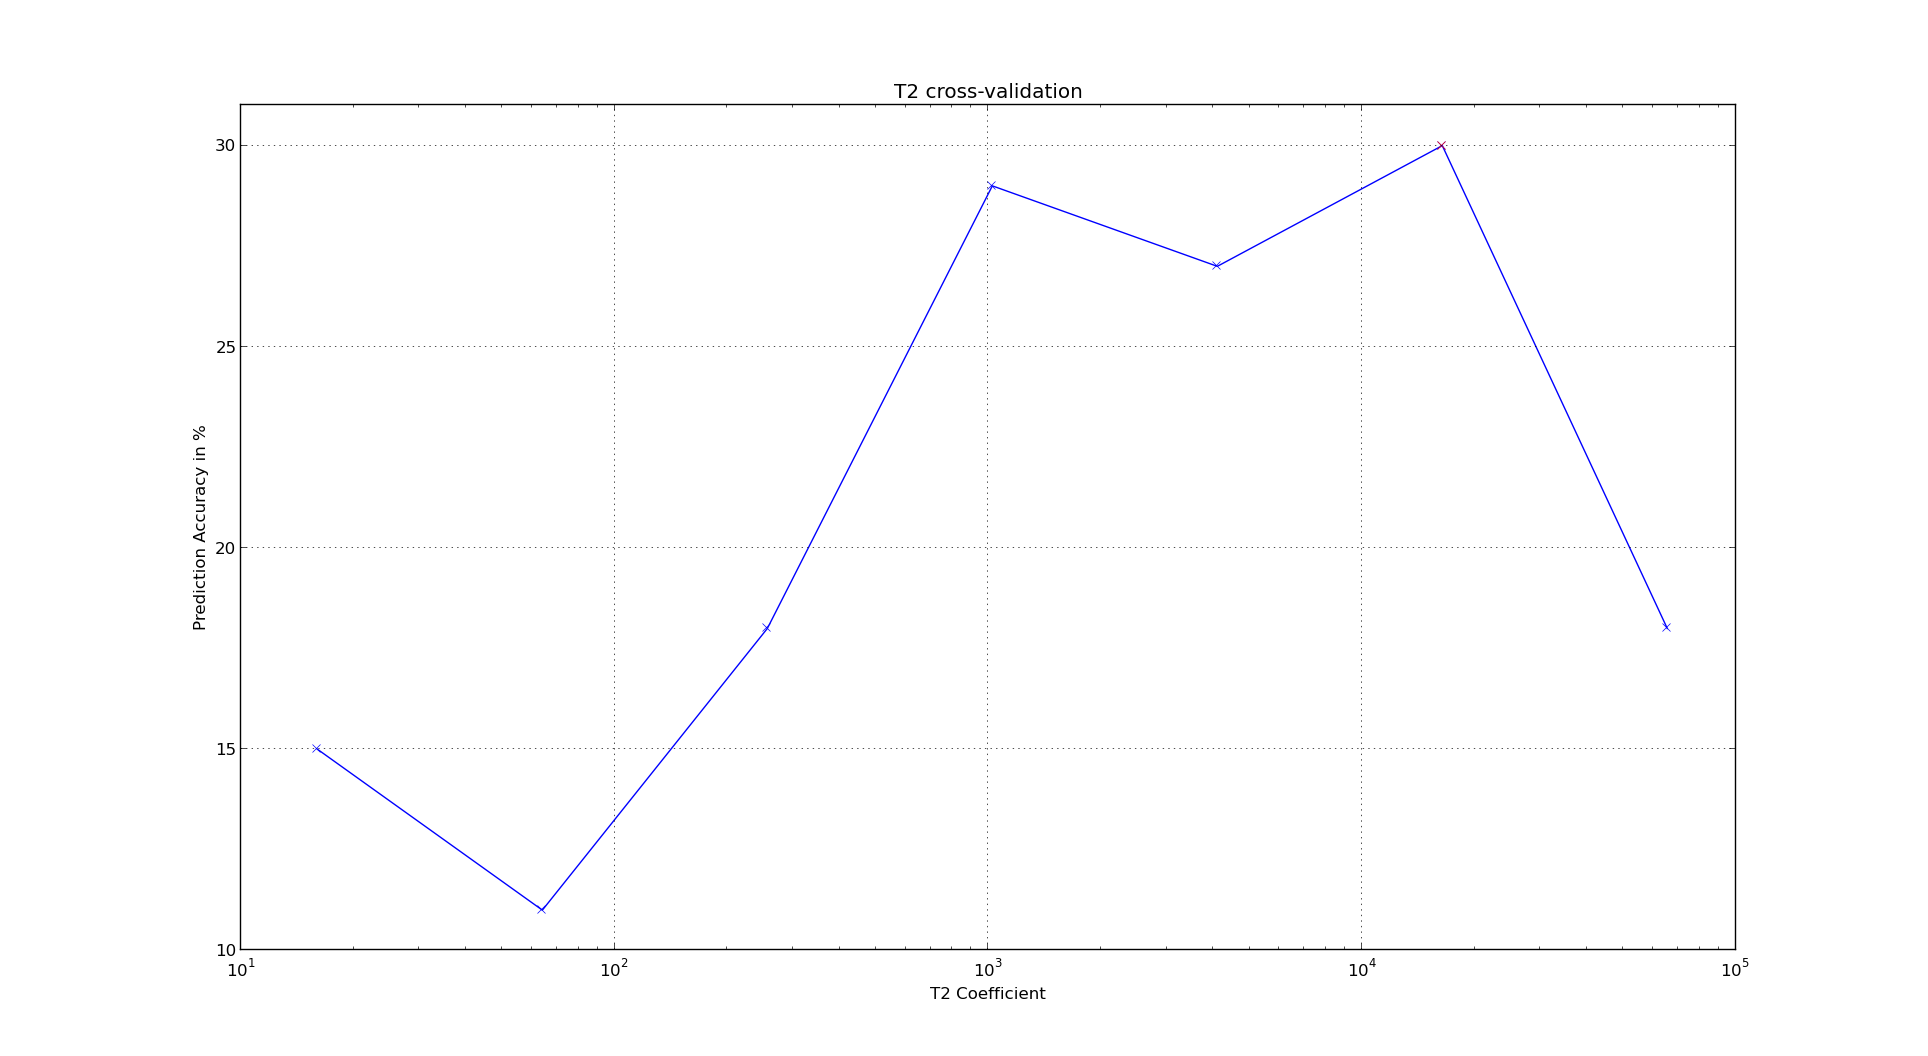
\includegraphics[scale=0.20]{cross_T2.png}\caption{Cross-validation of the $T_2$ coefficient : $16384$ with $30\%$}\label{figure4}
\end{center}
\end{figure}
The shape clearly indicates that a too small $T_2$ makes the discriminative information non relevant from the noise, while with higher $T$ we can have better contrast until we reach a point where once again the invariance implies the loss of discriminative information.
\subsection{Cross-validation : features}
The features computed have to be cross-validated :
\begin{figure}[H]
\begin{center}
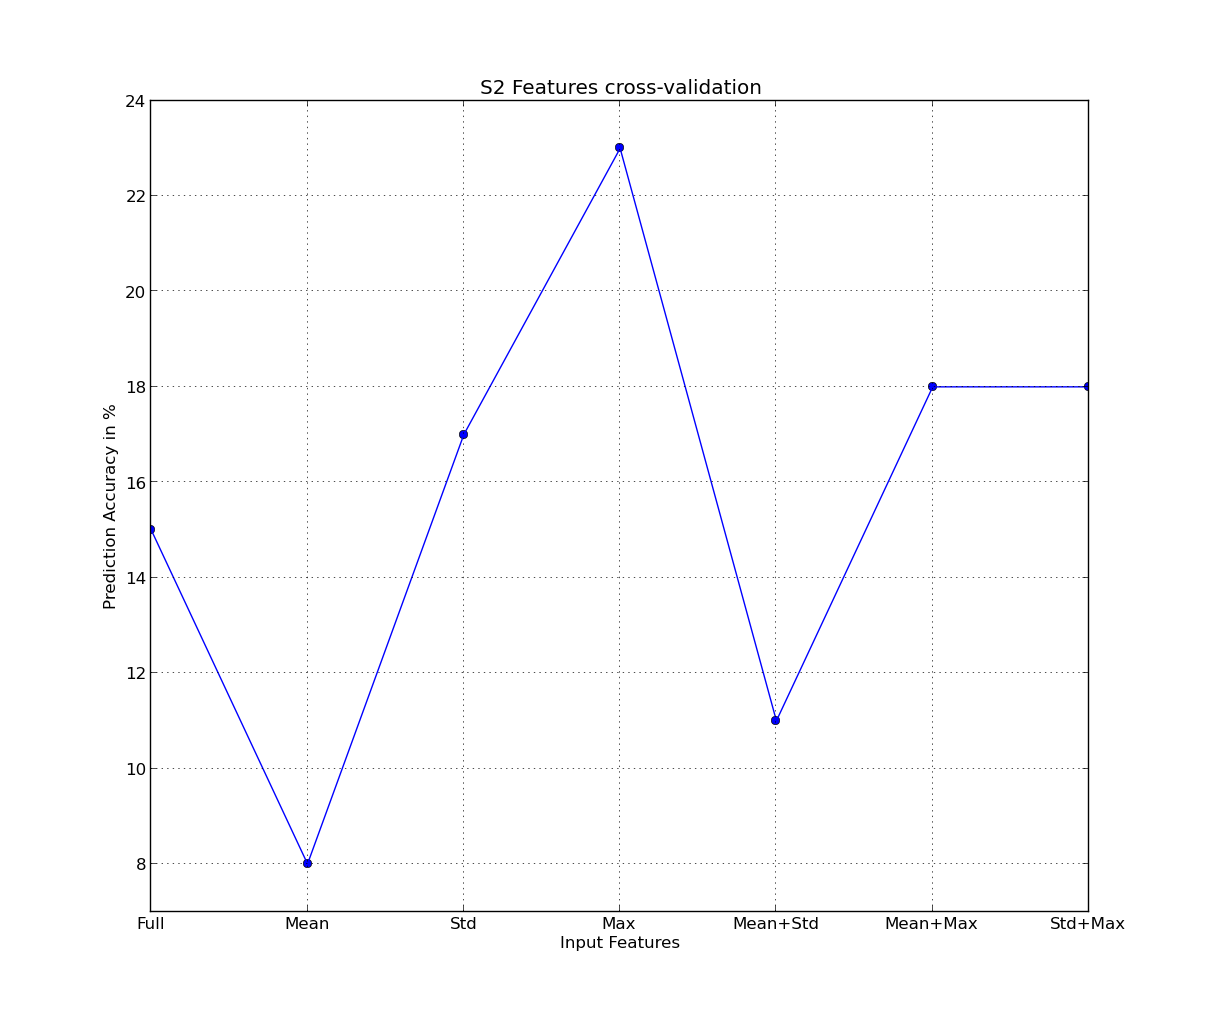
\includegraphics[scale=0.20]{S1_cross.png}\caption{Cross-validation of $S_1$ Features}\label{figure4}
\end{center}
\end{figure}
It is interesting to note that the mean features always seem to be far behind, but also that the full vector has a dimension of $1280*3$ and is still better than the mean alone thus the dimensionality reduction by a factor of $3$ doesn't compensate the loss of information induced by not using either the max or the std coefficients.\\

Now we can also try to add the coefficients of the first scattering layer leading to a feature vector with basically $[std(S_1),max(S_2)]$. The dimension will be greater by $80$ coefficients so we have a feature vector of size $80+80*2*8$.
\begin{figure}[H]
\begin{center}
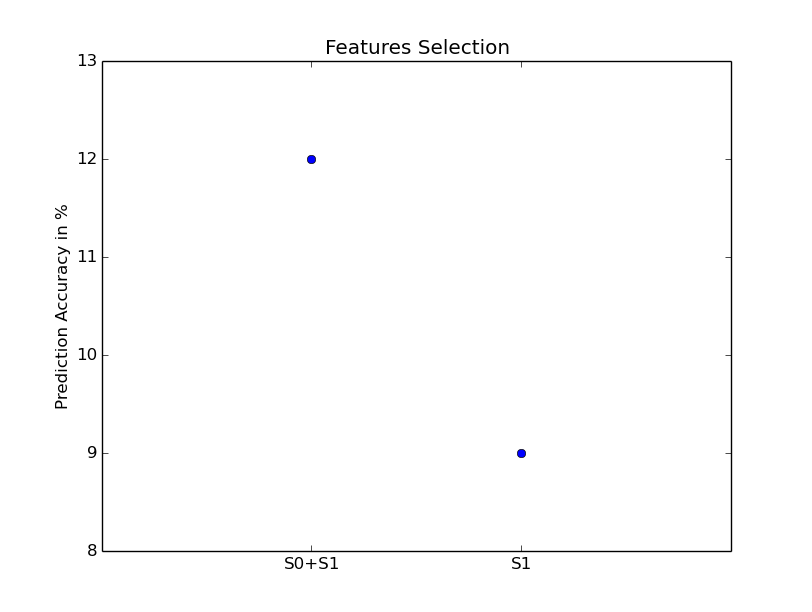
\includegraphics[scale=0.20]{S0_S1.png}\caption{Accruacy after adding the first scattering layer}\label{figure4}
\end{center}
\end{figure}
We will then keep this version of the algorithm by using informations from the first layer and the second layer. This is natural since we need both to keep the information about the signal. For example when looking at reconstruction problems, the coefficients of all the layers have to be kept in order to have better reconstructions.
\subsection{Cross-validation neurons}
We now cross-validate the remaining coefficients : the number of hidden neurons in the neural network.
\begin{figure}[H]
\begin{center}
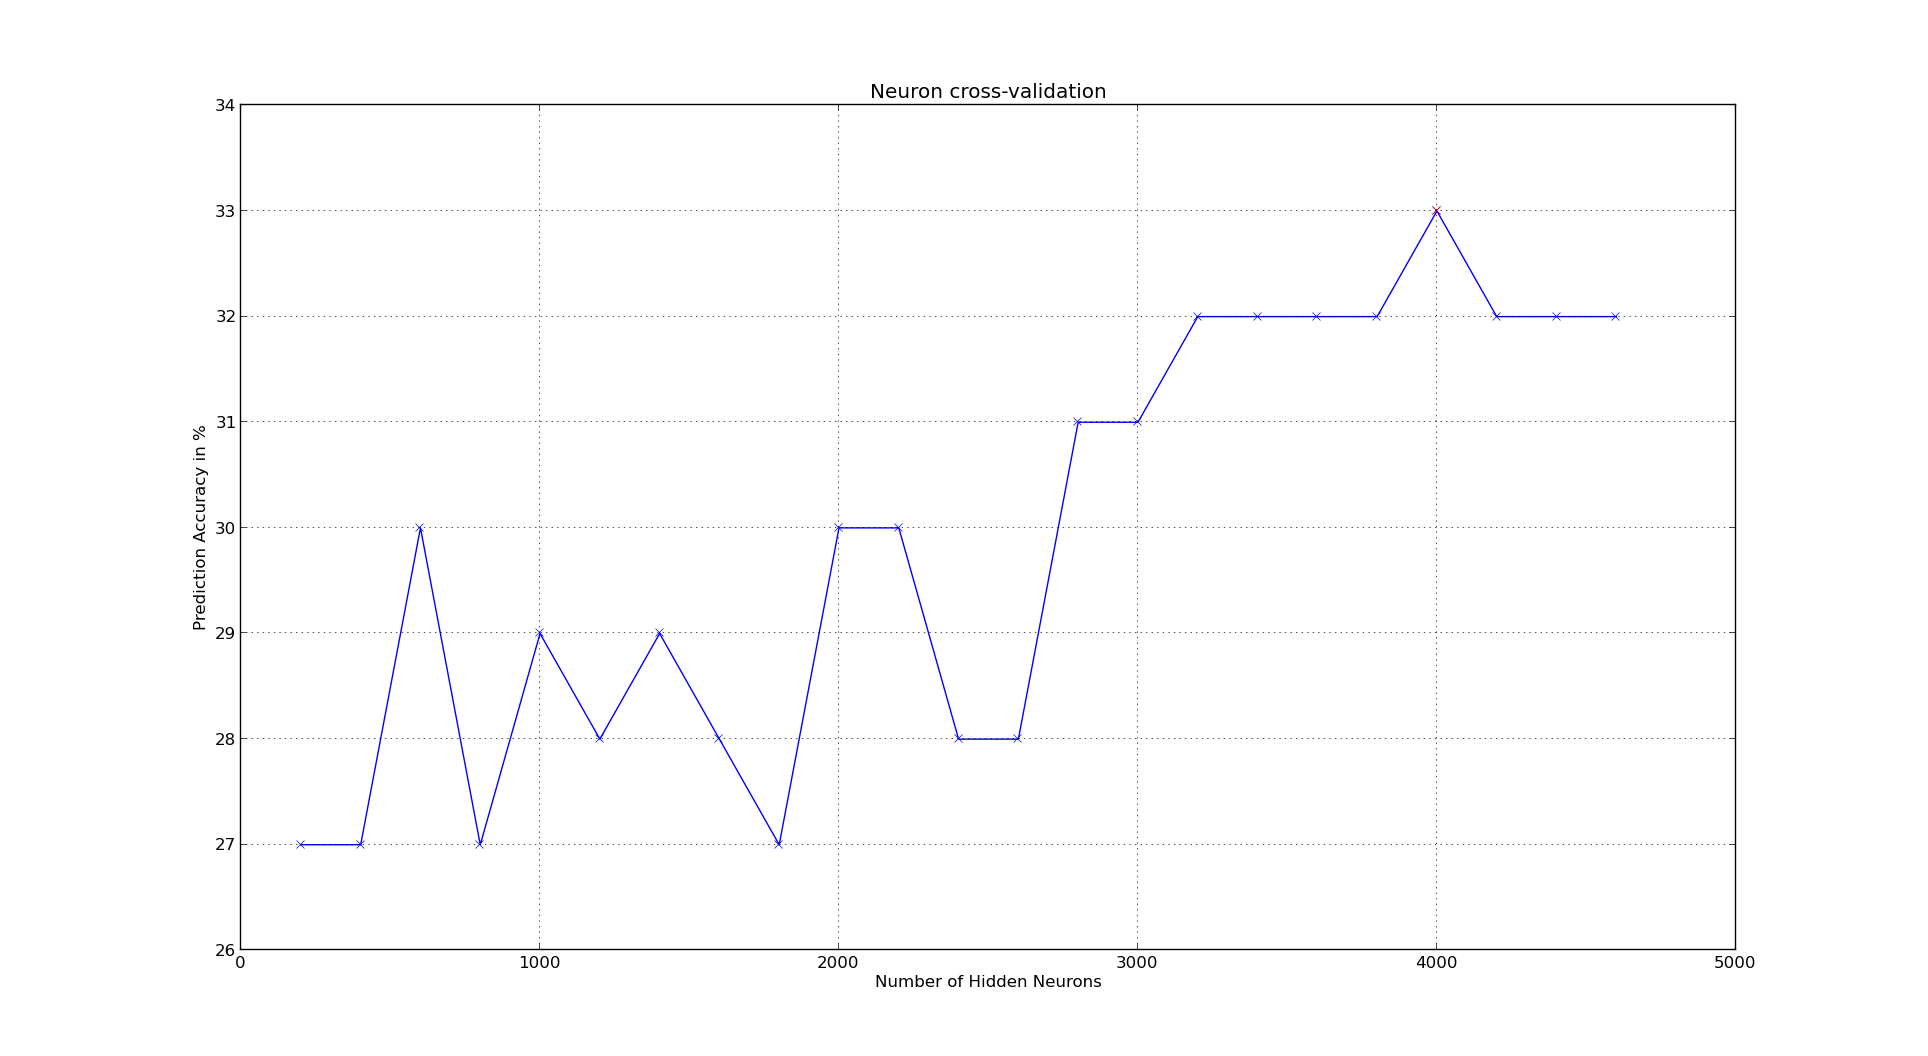
\includegraphics[scale=0.20]{cross_neuron_S0_S1.png}\caption{Cross-validation on the number of Hidden Neurons}\label{figure4}
\end{center}
\end{figure}
\subsection{Results Summary and Discussions}
By using two layers we are able to reach an accuracy of $33\%$ for $45$ classes using a feature vector of size $1280+80$ which is reasonable. We can already see that the feature vector should have the minimum size possible with the maximum amount of discriminative information. 
\\
It is clear that the parameters $Q_2$ and $J_2$ are sub-optimal. However, the option to optimize simultaneously all the filter bank coefficients ($T_2$, $Q_2$, $J_2$) involves high level machine learning techniques and wasn't used.
\\
Finally, the accuracy gain (compared to the accuracy of the one layer architecture) doesn't justify the use of a second scattering layer. The reason for this small improvement is also the dimension of the feature vector compared to the information gain.\\
One way to mitigate this problem might be to use some sort of dimensionality reduction on this second scattering layer through a possible hard thresholding (we aim to eliminate the values not coding information about the birds for example).
\section{Two Layers with $U_2$ Thresholding}
\subsection{Architecture}
The aim of this new approach is to combine the information gain of the second scattering layer while finding the best compromise between dimensionality and information. In order to do so a natural approach is to see that not all the $\psi_{2,\lambda_2}$ filters are suited to encode the bird song behaviours. It is then natural to try to put some kind of thresholding at this level.  Multiple approaches can be used. The one used here is to simply make a linear combination of the $U_2$ decomposition with respect to the $\psi_{2,\lambda_2}$ filters. Another approach could be to directly find the best wavelets for the second layer through some sparse coding techniques for example.\\
 Let's see the scheme :
\begin{equation}
\begin{array}{c c c}
U_2(\lambda_1, \lambda_2,t)& \rightarrow &U'_2(\lambda_1,k(\lambda_2),t) \\
& & \downarrow \\
& & |U'_2 \star \psi_{\lambda_3}| := U'_3(\lambda_1, k(\lambda_2),\lambda_3,t) \\
& & \downarrow \\
& & U'_3 \star \phi_3 := S'_3(\lambda_1, k(\lambda_2),\lambda_3,t)\\
\end{array}
\end{equation}
Where we have, using the previous notations :
\[
U'_2(\lambda_1,k(\lambda_2),t)=
\sum_{i=1}^{\lambda_2}k_i*U_2(\lambda_1,i,t)
\]
\[
U'_2 \in \mathbb{R}^{| \lambda_1| \times N}
\]

Clearly the point is not only to reduce the dimension but also to introduce some thresholding (by weighting the contribution of the given $\psi_{2,\lambda_2}$ with a $\beta_i$. The set of weighting coefficients can be optimized by multiple techniques. The most natural one could be to try to find some clustering of the data vectors and to take the centroid properties for the weighting. Since the aim of this section is to prove the usefulness of this approach, only two sets of coefficients will be tested and compared. The first one is by taking all the coefficients equal to $1$ thus there are no thresholding but aggregation of the $\lambda_2$ component. The second approach will be done using $\beta_i$ of a pyramidal shape (attenuating the first and last $\psi_{2,\lambda_2}$ filters. Let's first look at some examples of what we are trying to threshold.


\subsection{Examples}

There are $3$ different signals and each time is presented the $U_2$ for each $\psi_{2,\lambda_2}$. The second plot is then a linear combination of these by groups of $3$. Note that these representations are made with the coefficients $Q_2=1,J_2=14$.


\begin{figure}[H]
\begin{center}
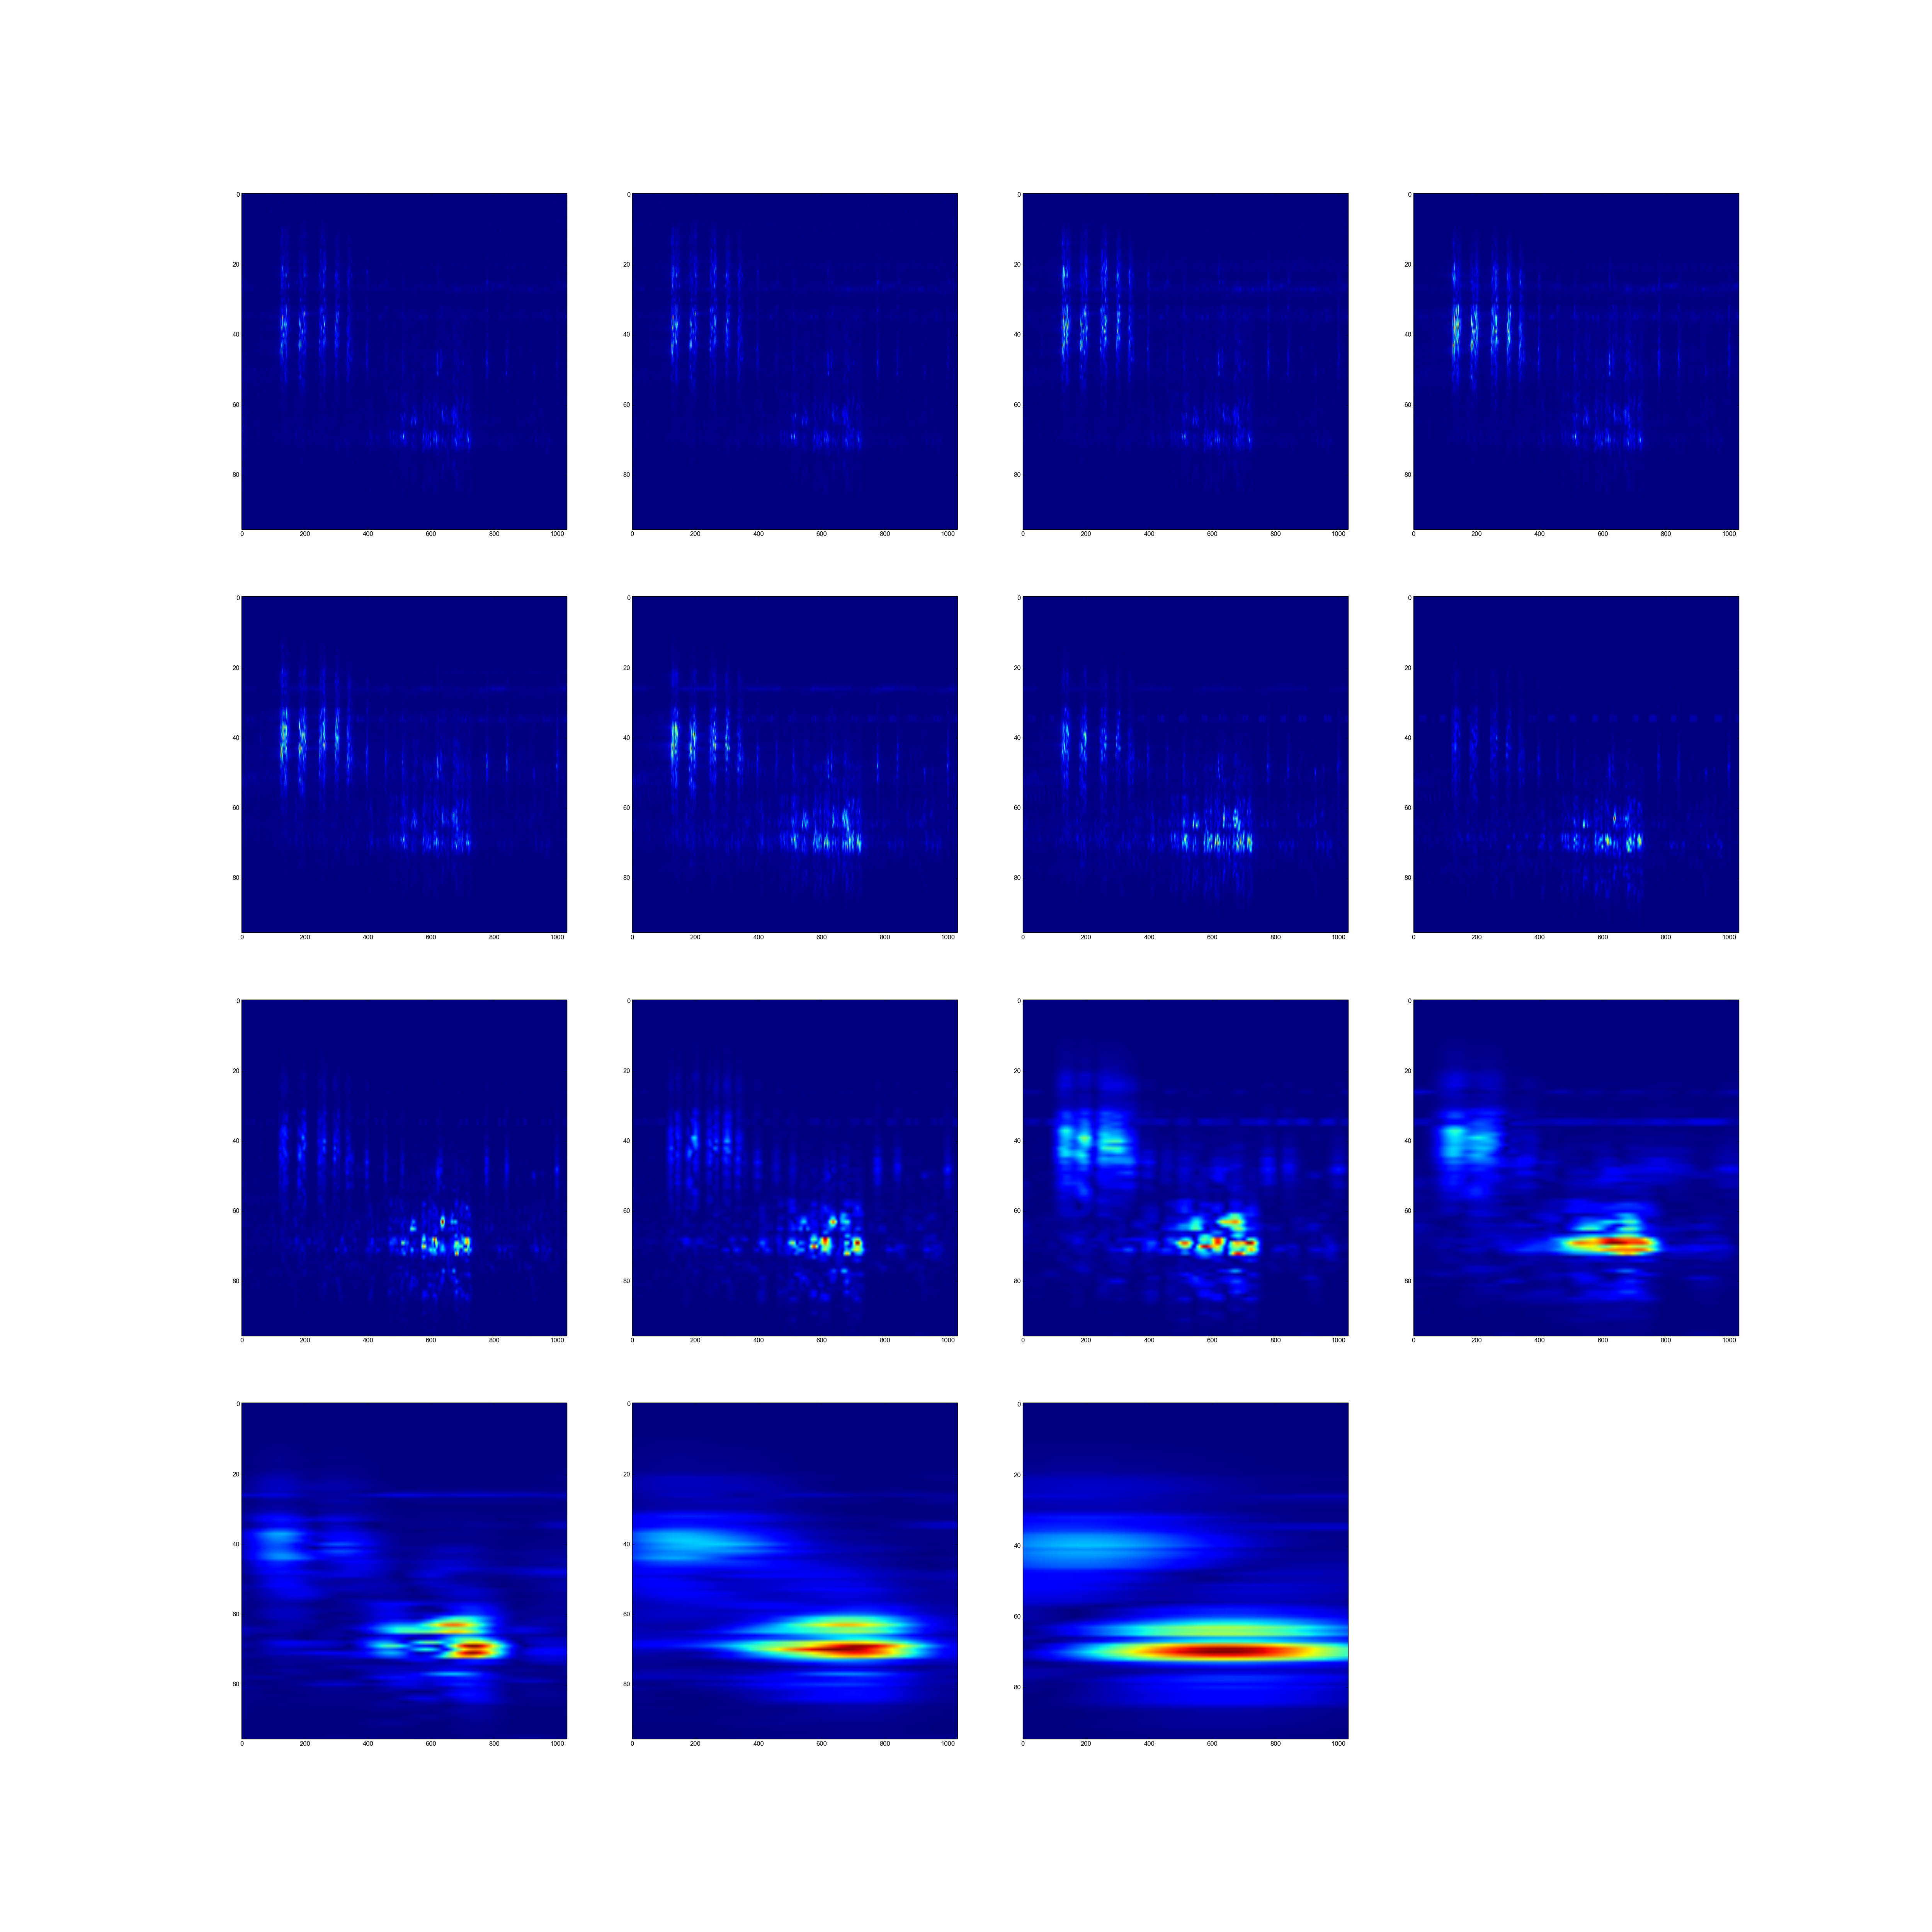
\includegraphics[scale=0.1]{RN5821_1.png}\caption{Signal name : RN5821.wav, each subplot $i=0,...,14$ represents $||x \star \psi_{1,\lambda_1}|\star \psi_{2,i}|$, the application of the $i^{th}$ $\psi$ filter of the second filter bank on $U_1$ which are then re-normalized independently.}
\end{center}
\end{figure}


\begin{figure}[H]
\begin{center}
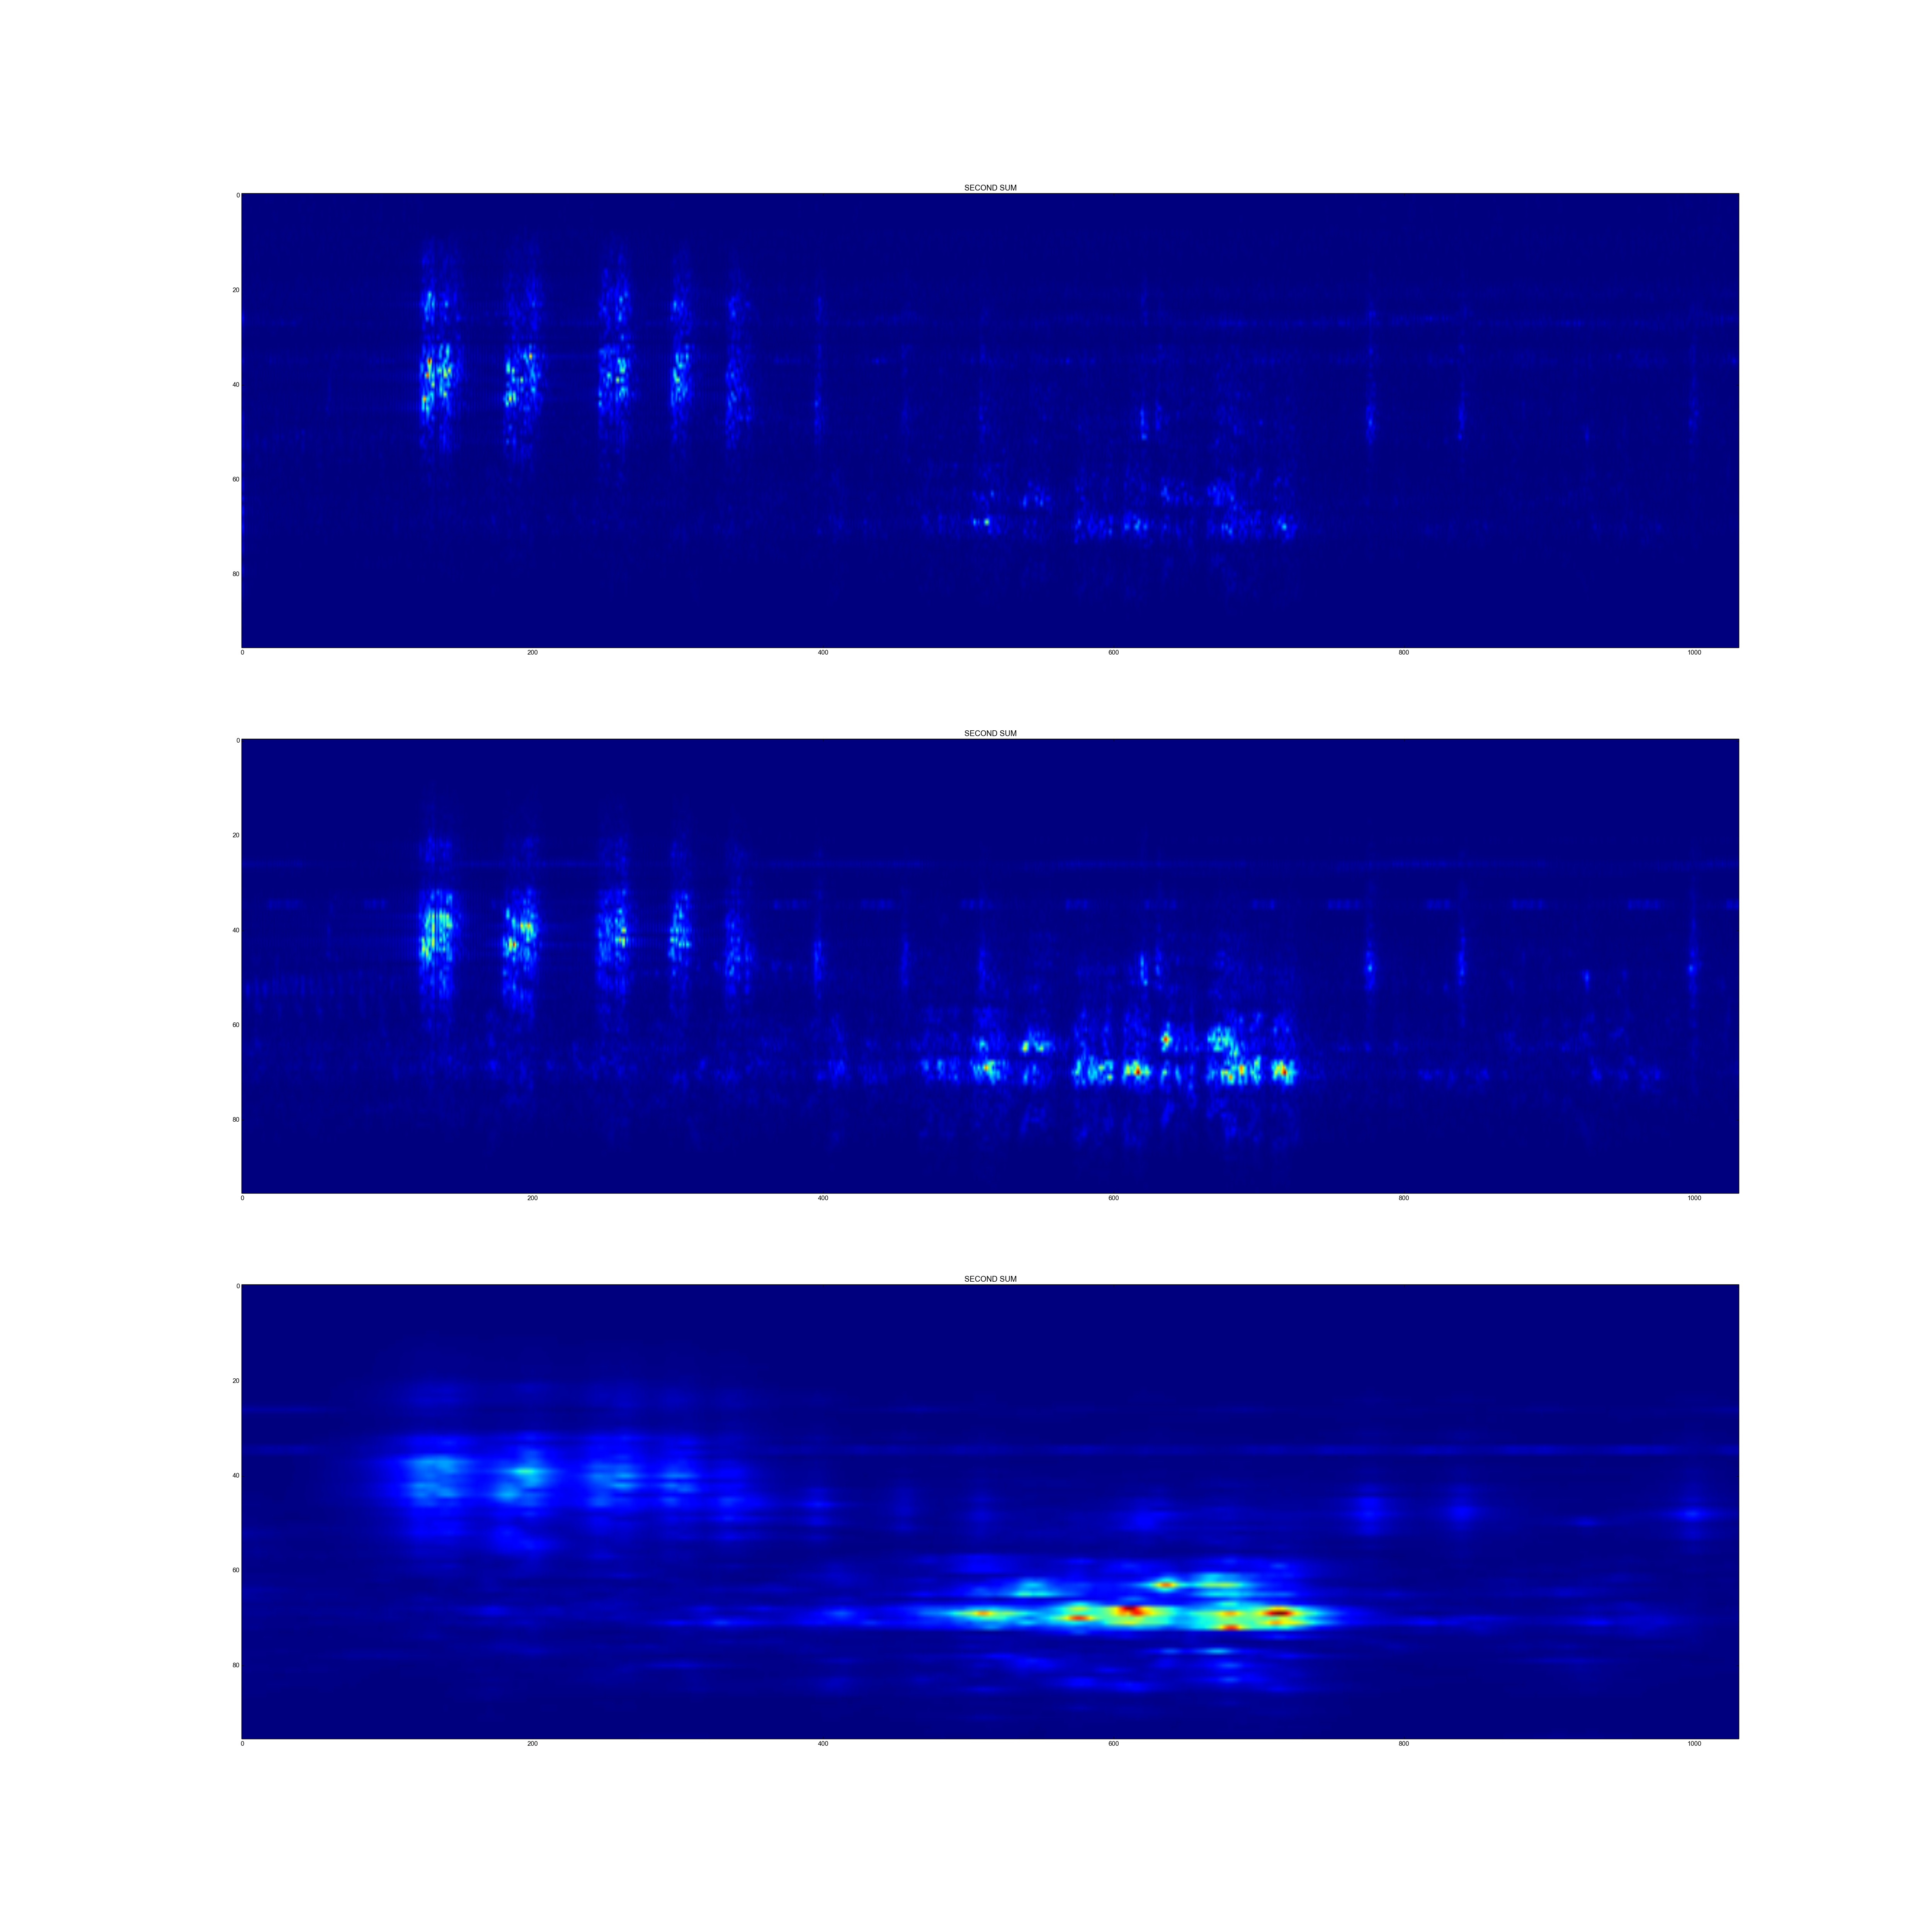
\includegraphics[scale=0.1]{RN5821_3.png}\caption{Each subplot $j=0,1,2$ is equal to $\sum_{i=0}^4 U_{2,j*5+i}$ representing an element wise addition of the previous subplots ($5$ by $5$ with $\beta_i=1\forall i$ so no thresholding of a particular $\psi_{2,i}$) }
\end{center}
\end{figure}


\begin{figure}[H]
\begin{center}
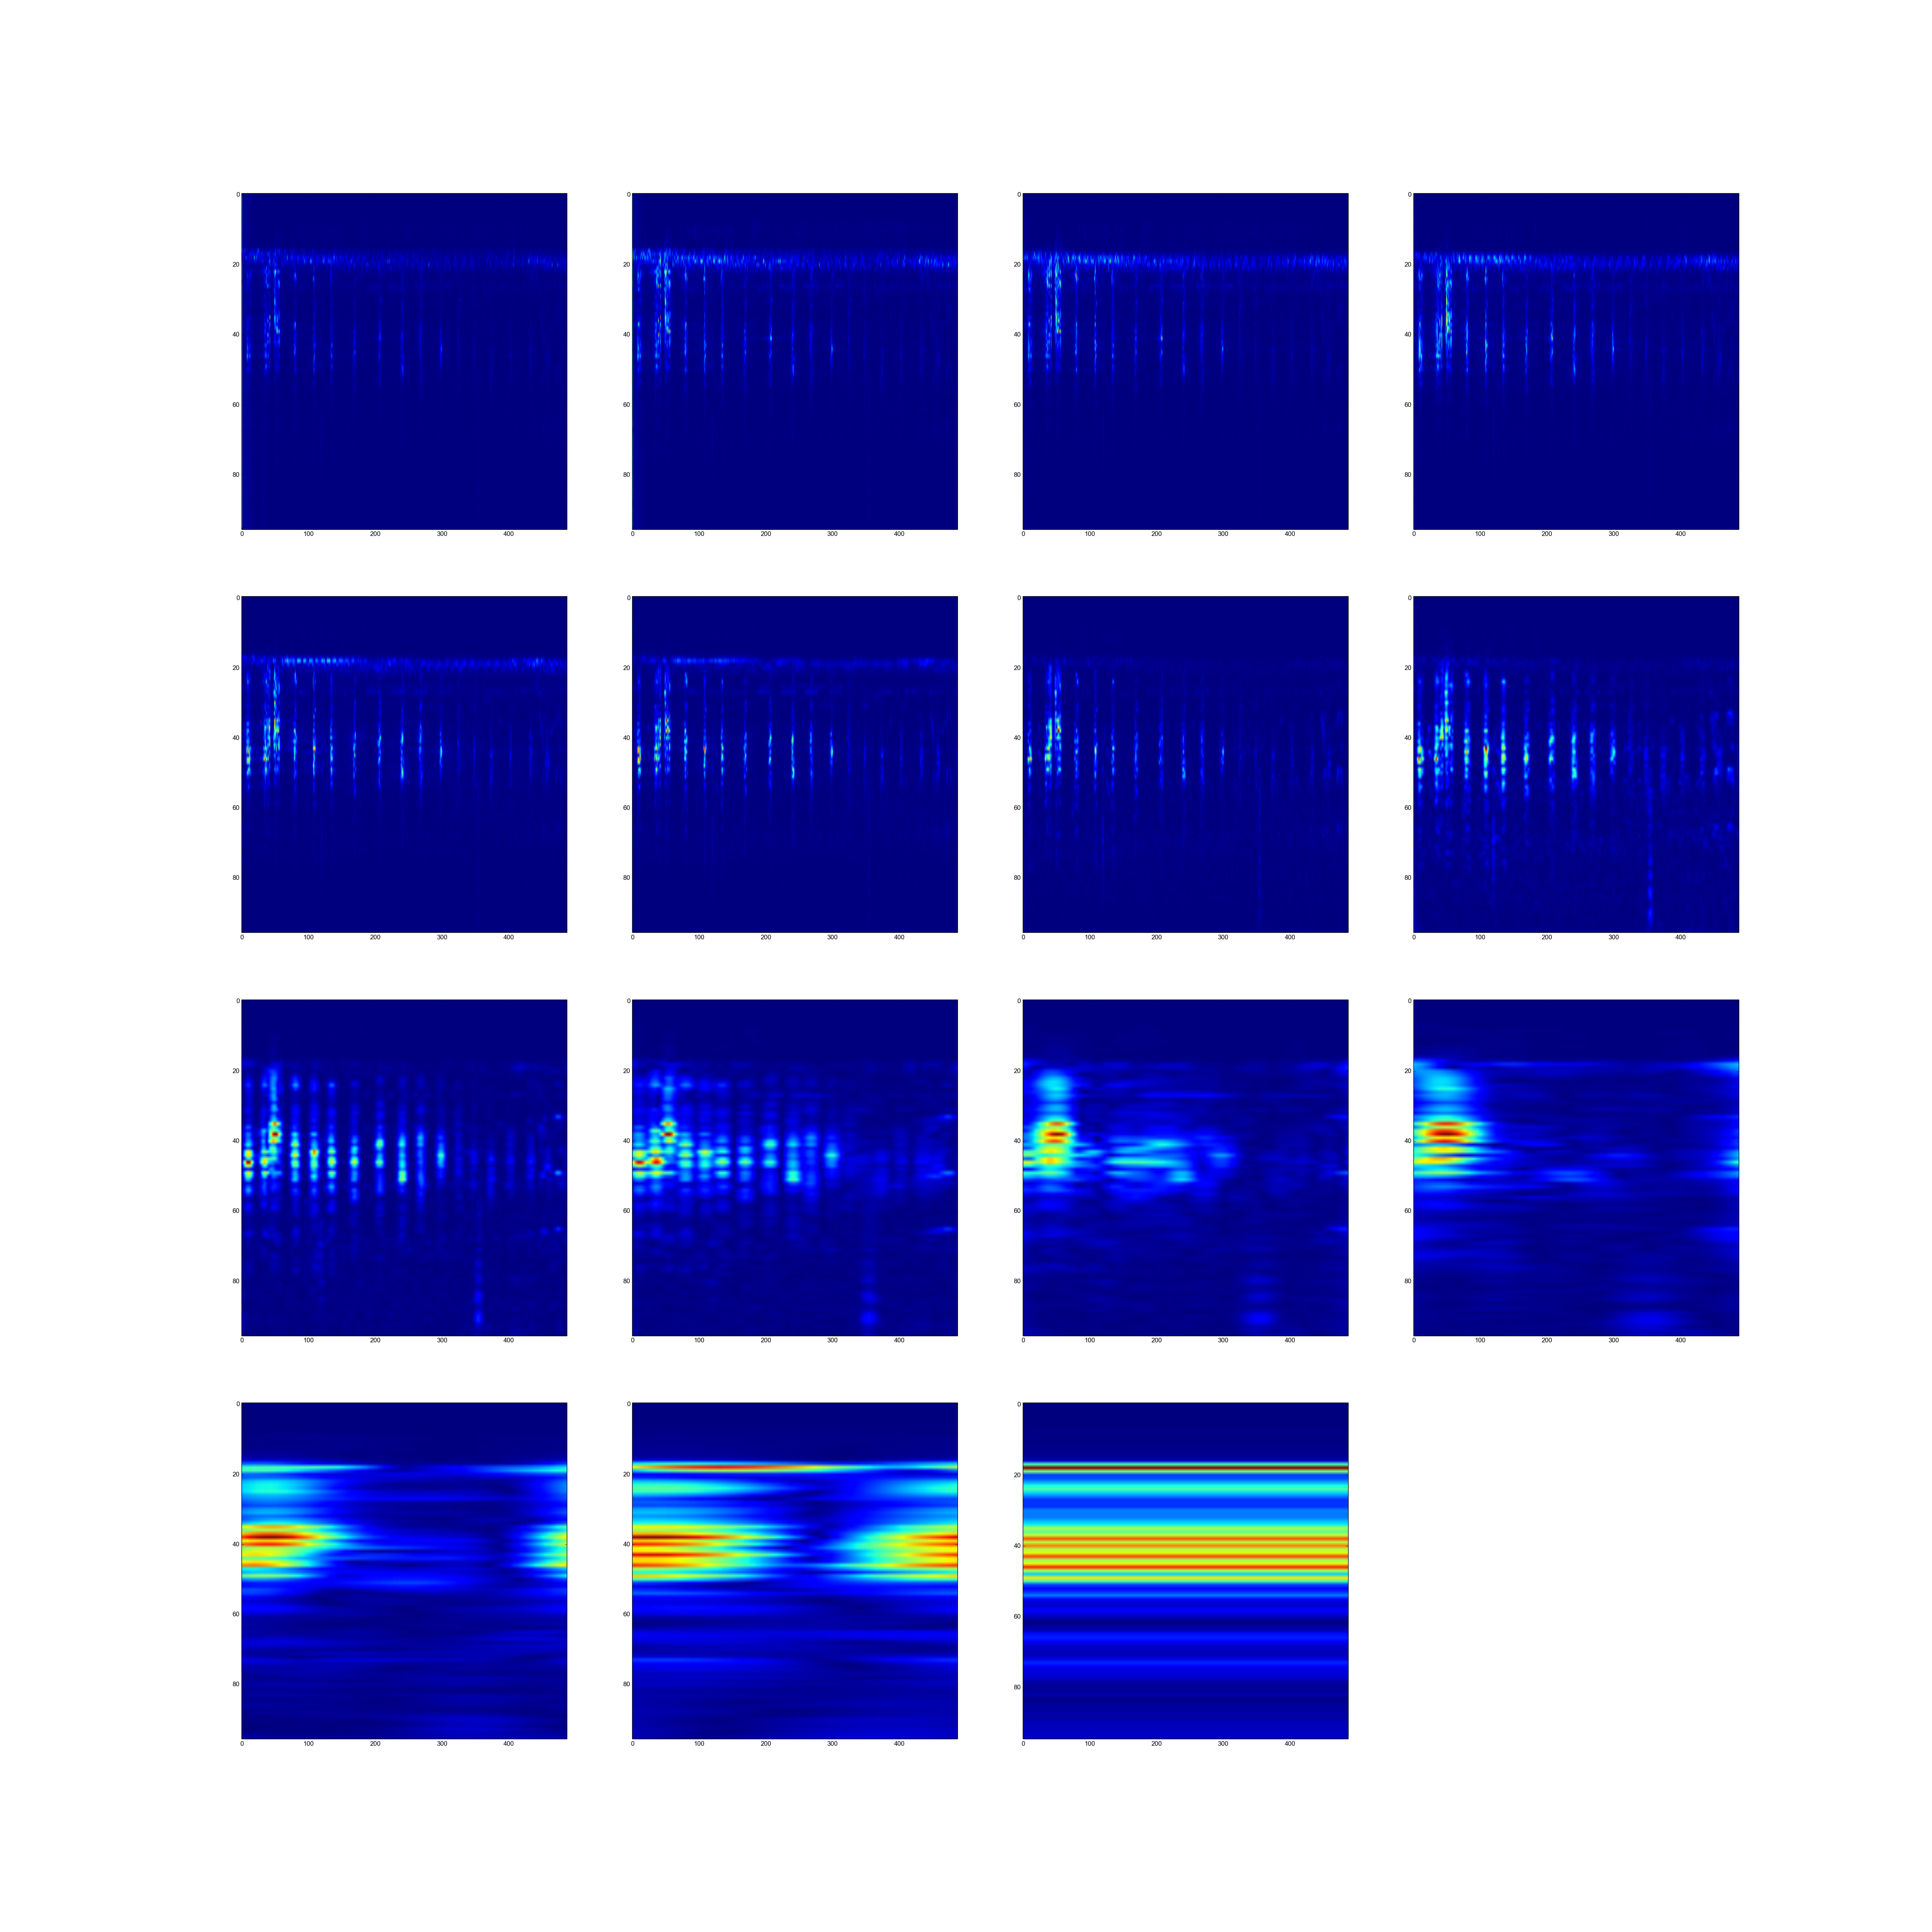
\includegraphics[scale=0.1]{RN1017_1.png}\caption{Signal name : RN1017.wav, each subplot $i=0,...,14$ represents $||x \star \psi_{1,\lambda_1}|\star \psi_{2,i}|$, the application of the $i^{th}$ $\psi$ filter of the second filter bank on $U_1$ which are then re-normalized independently.}
\end{center}
\end{figure}

\begin{figure}[H]
\begin{center}
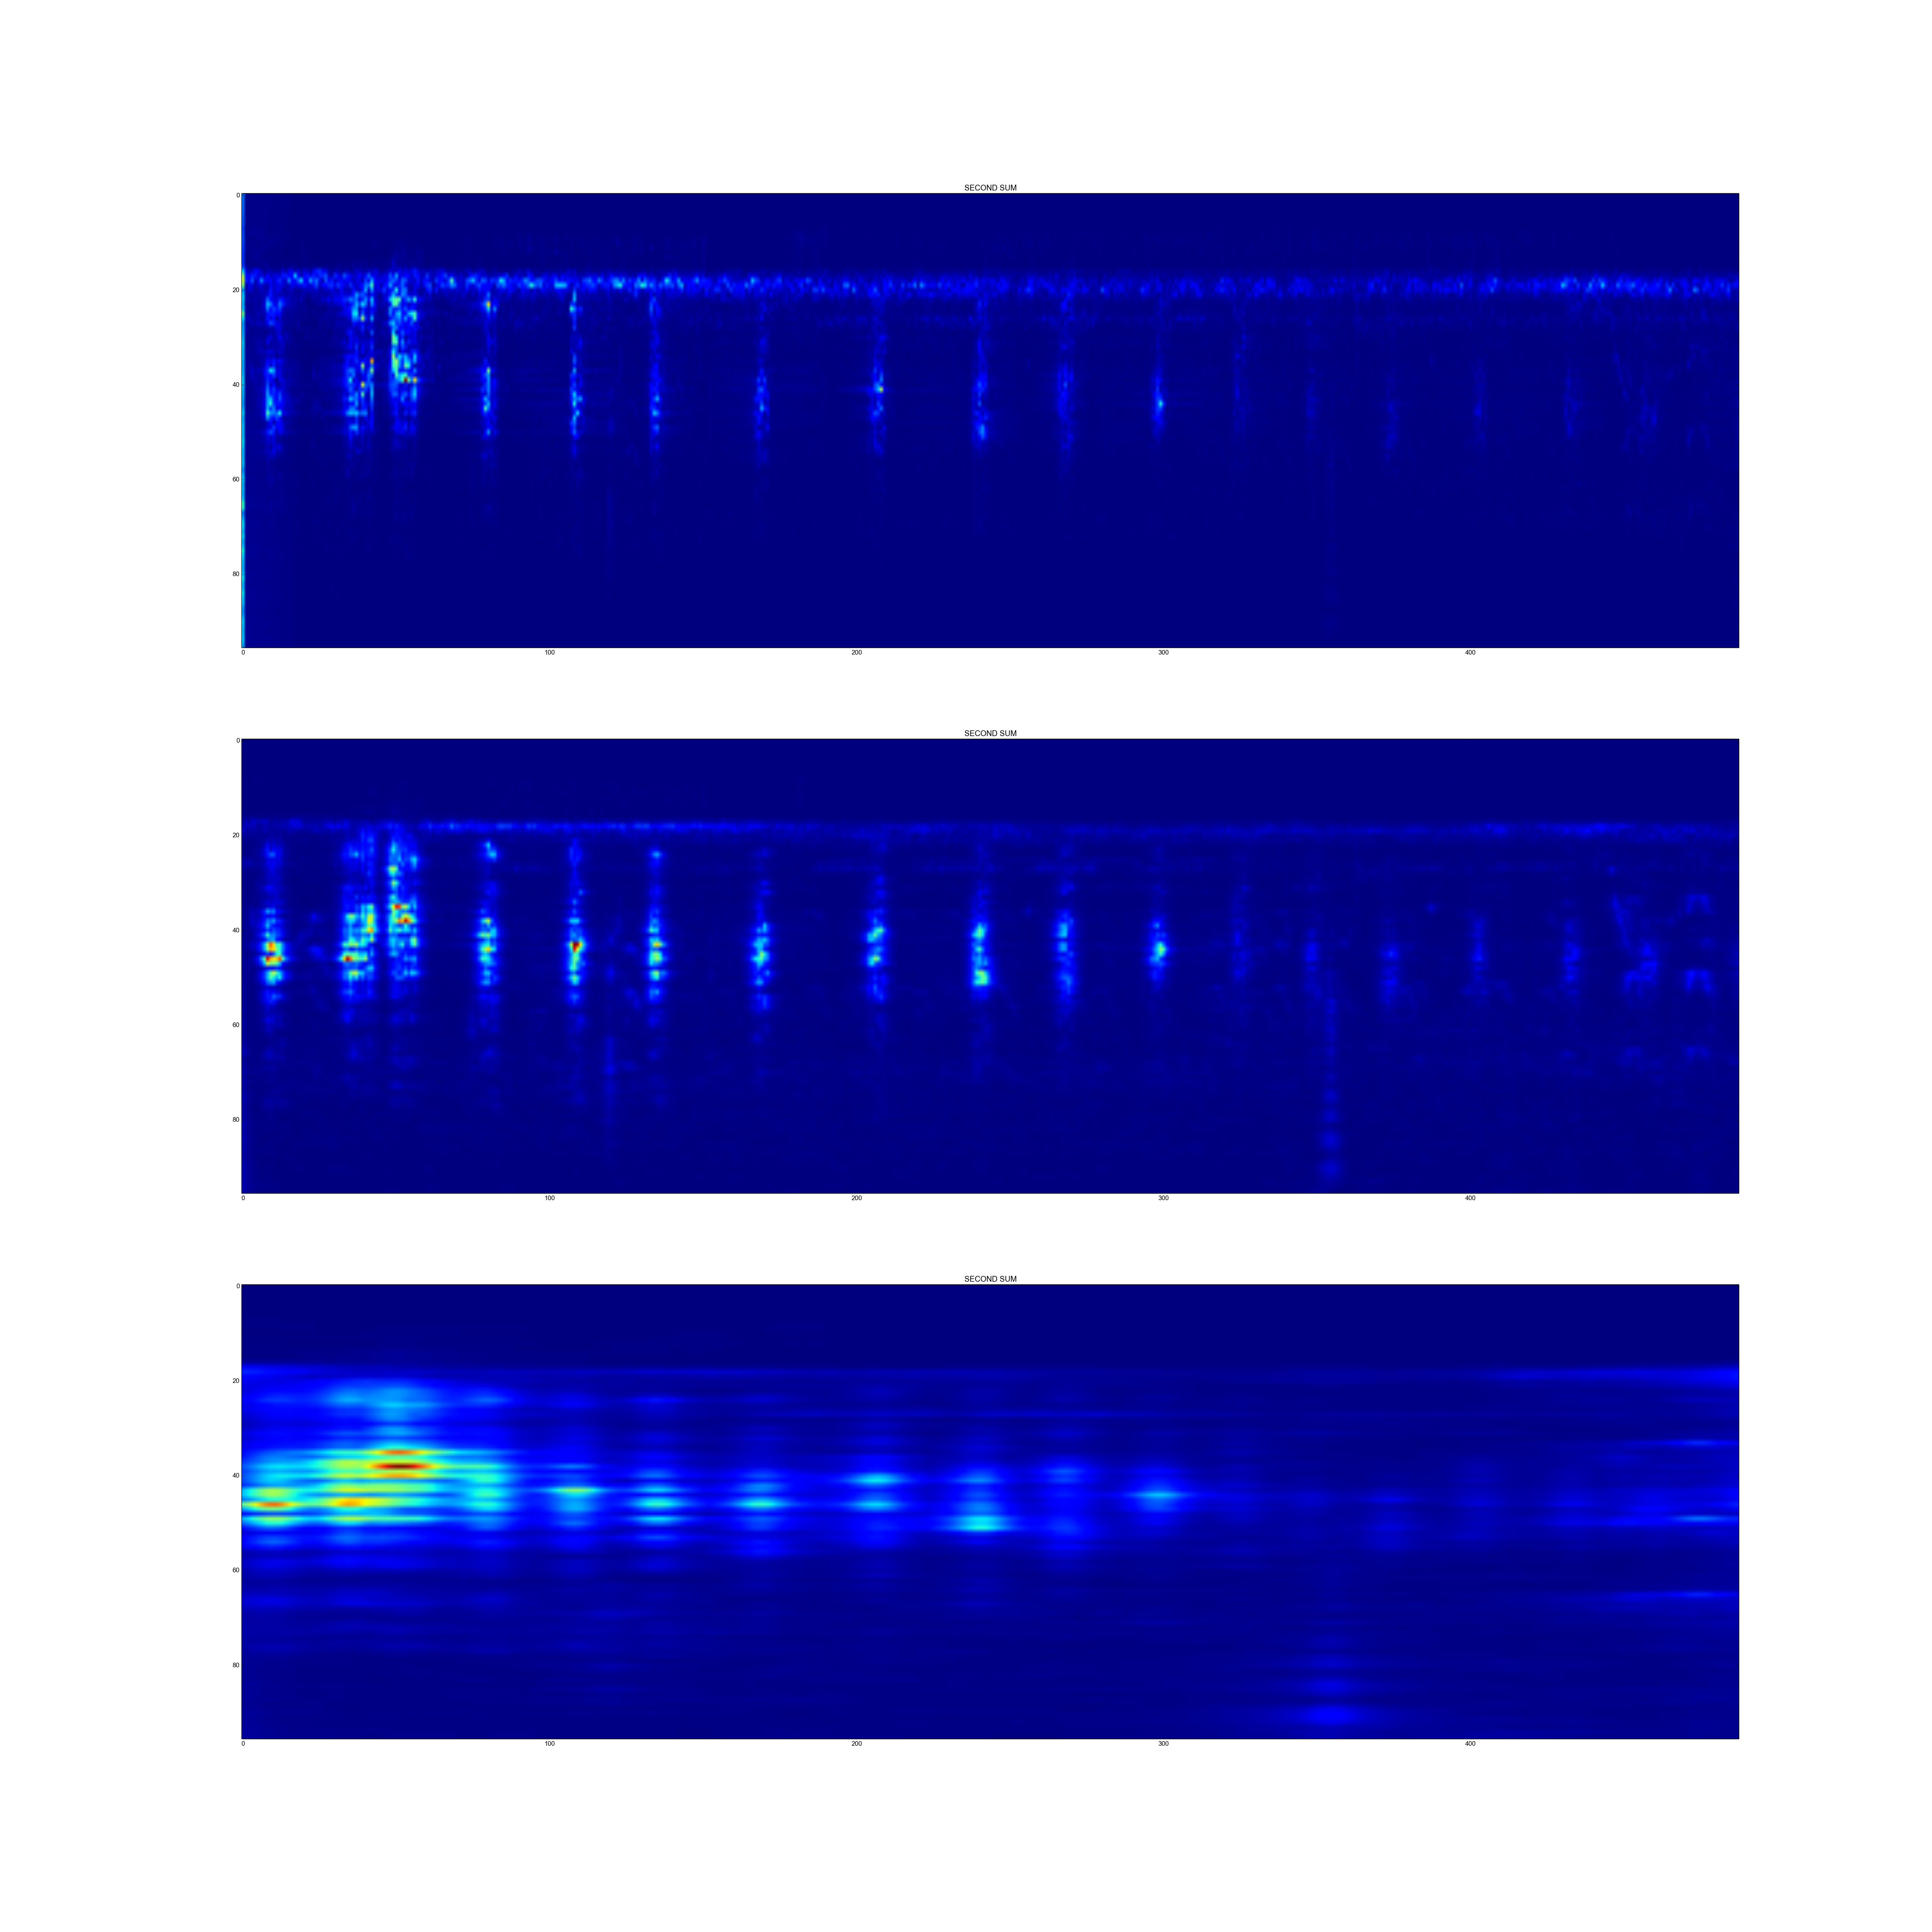
\includegraphics[scale=0.1]{RN1017_3.png}\caption{Each subplot $j=0,1,2$ is equal to $\sum_{i=0}^4 U_{2,j*5+i}$ representing an element wise addition of the previous subplots ($5$ by $5$ with $\beta_i=1\forall i$ so no thresholding of a particular $\psi_{2,i}$) }
\end{center}
\end{figure}


\begin{figure}[H]
\begin{center}
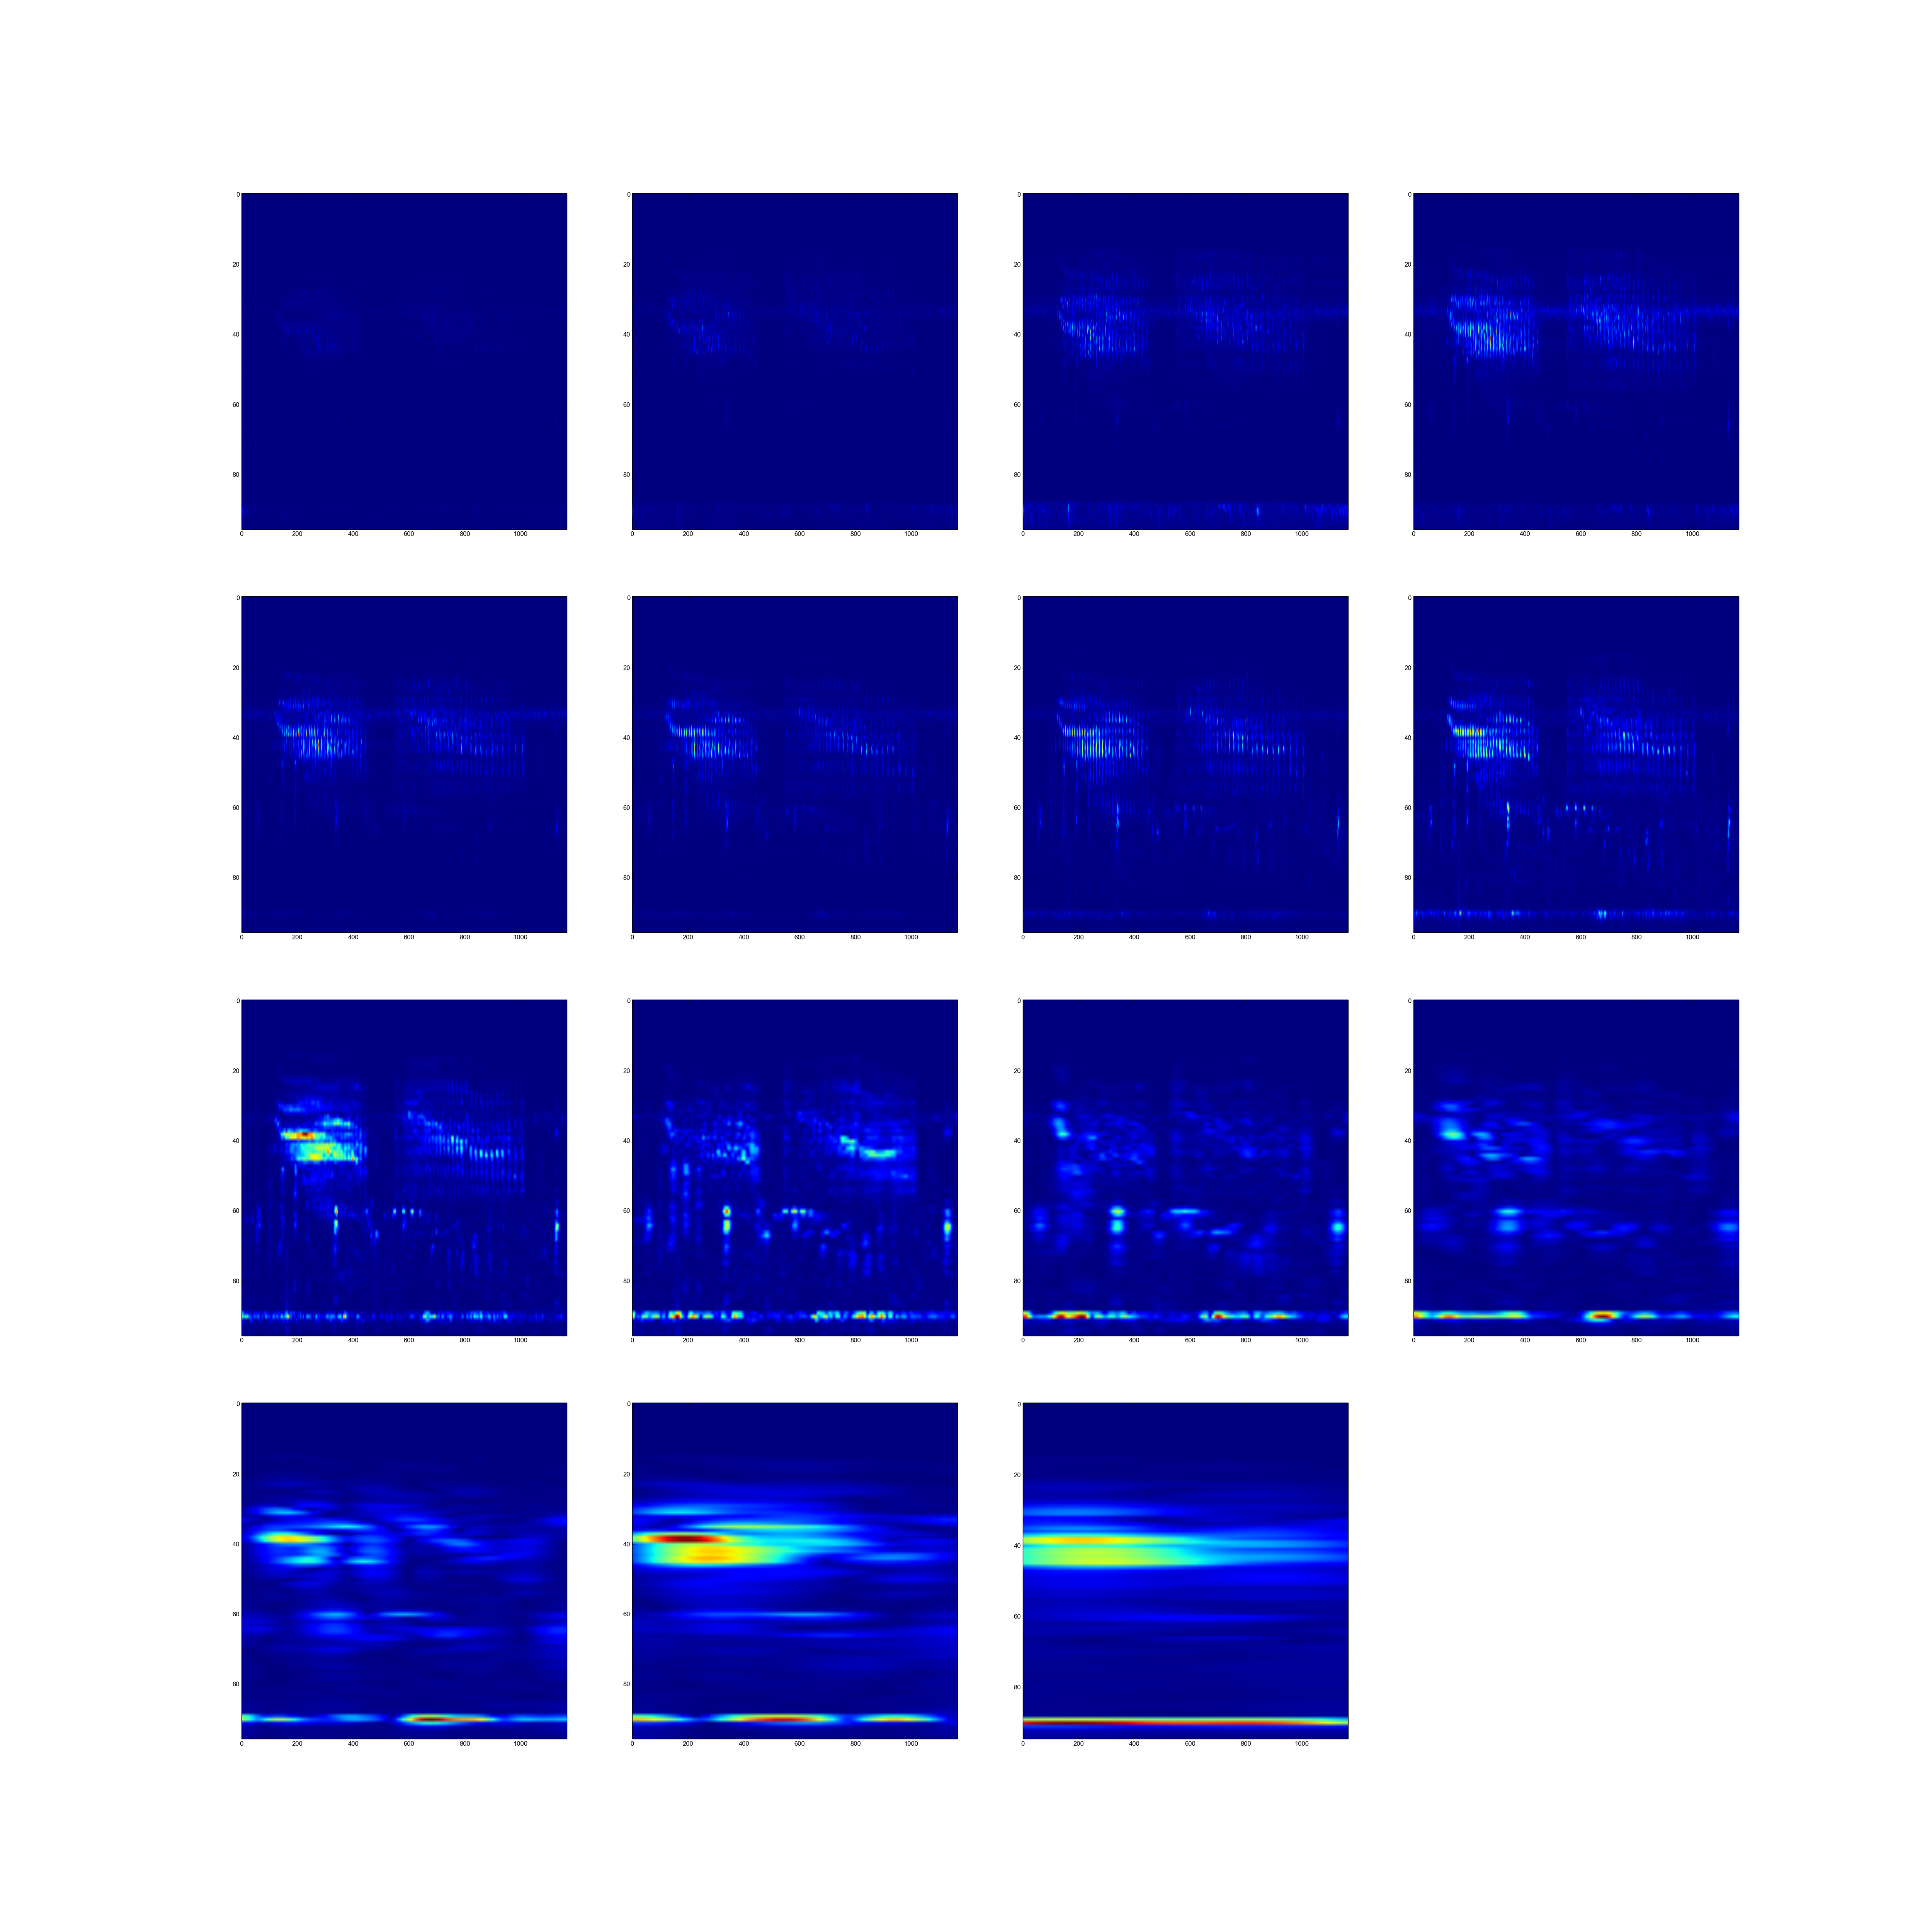
\includegraphics[scale=0.1]{RN819_1.png}\caption{Signal name : RN819.wav, each subplot $i=0,...,14$ represents $||x \star \psi_{1,\lambda_1}|\star \psi_{2,i}|$, the application of the $i^{th}$ $\psi$ filter of the second filter bank on $U_1$ which are then re-normalized independently.}
\end{center}
\end{figure}

\begin{figure}[H]
\begin{center}
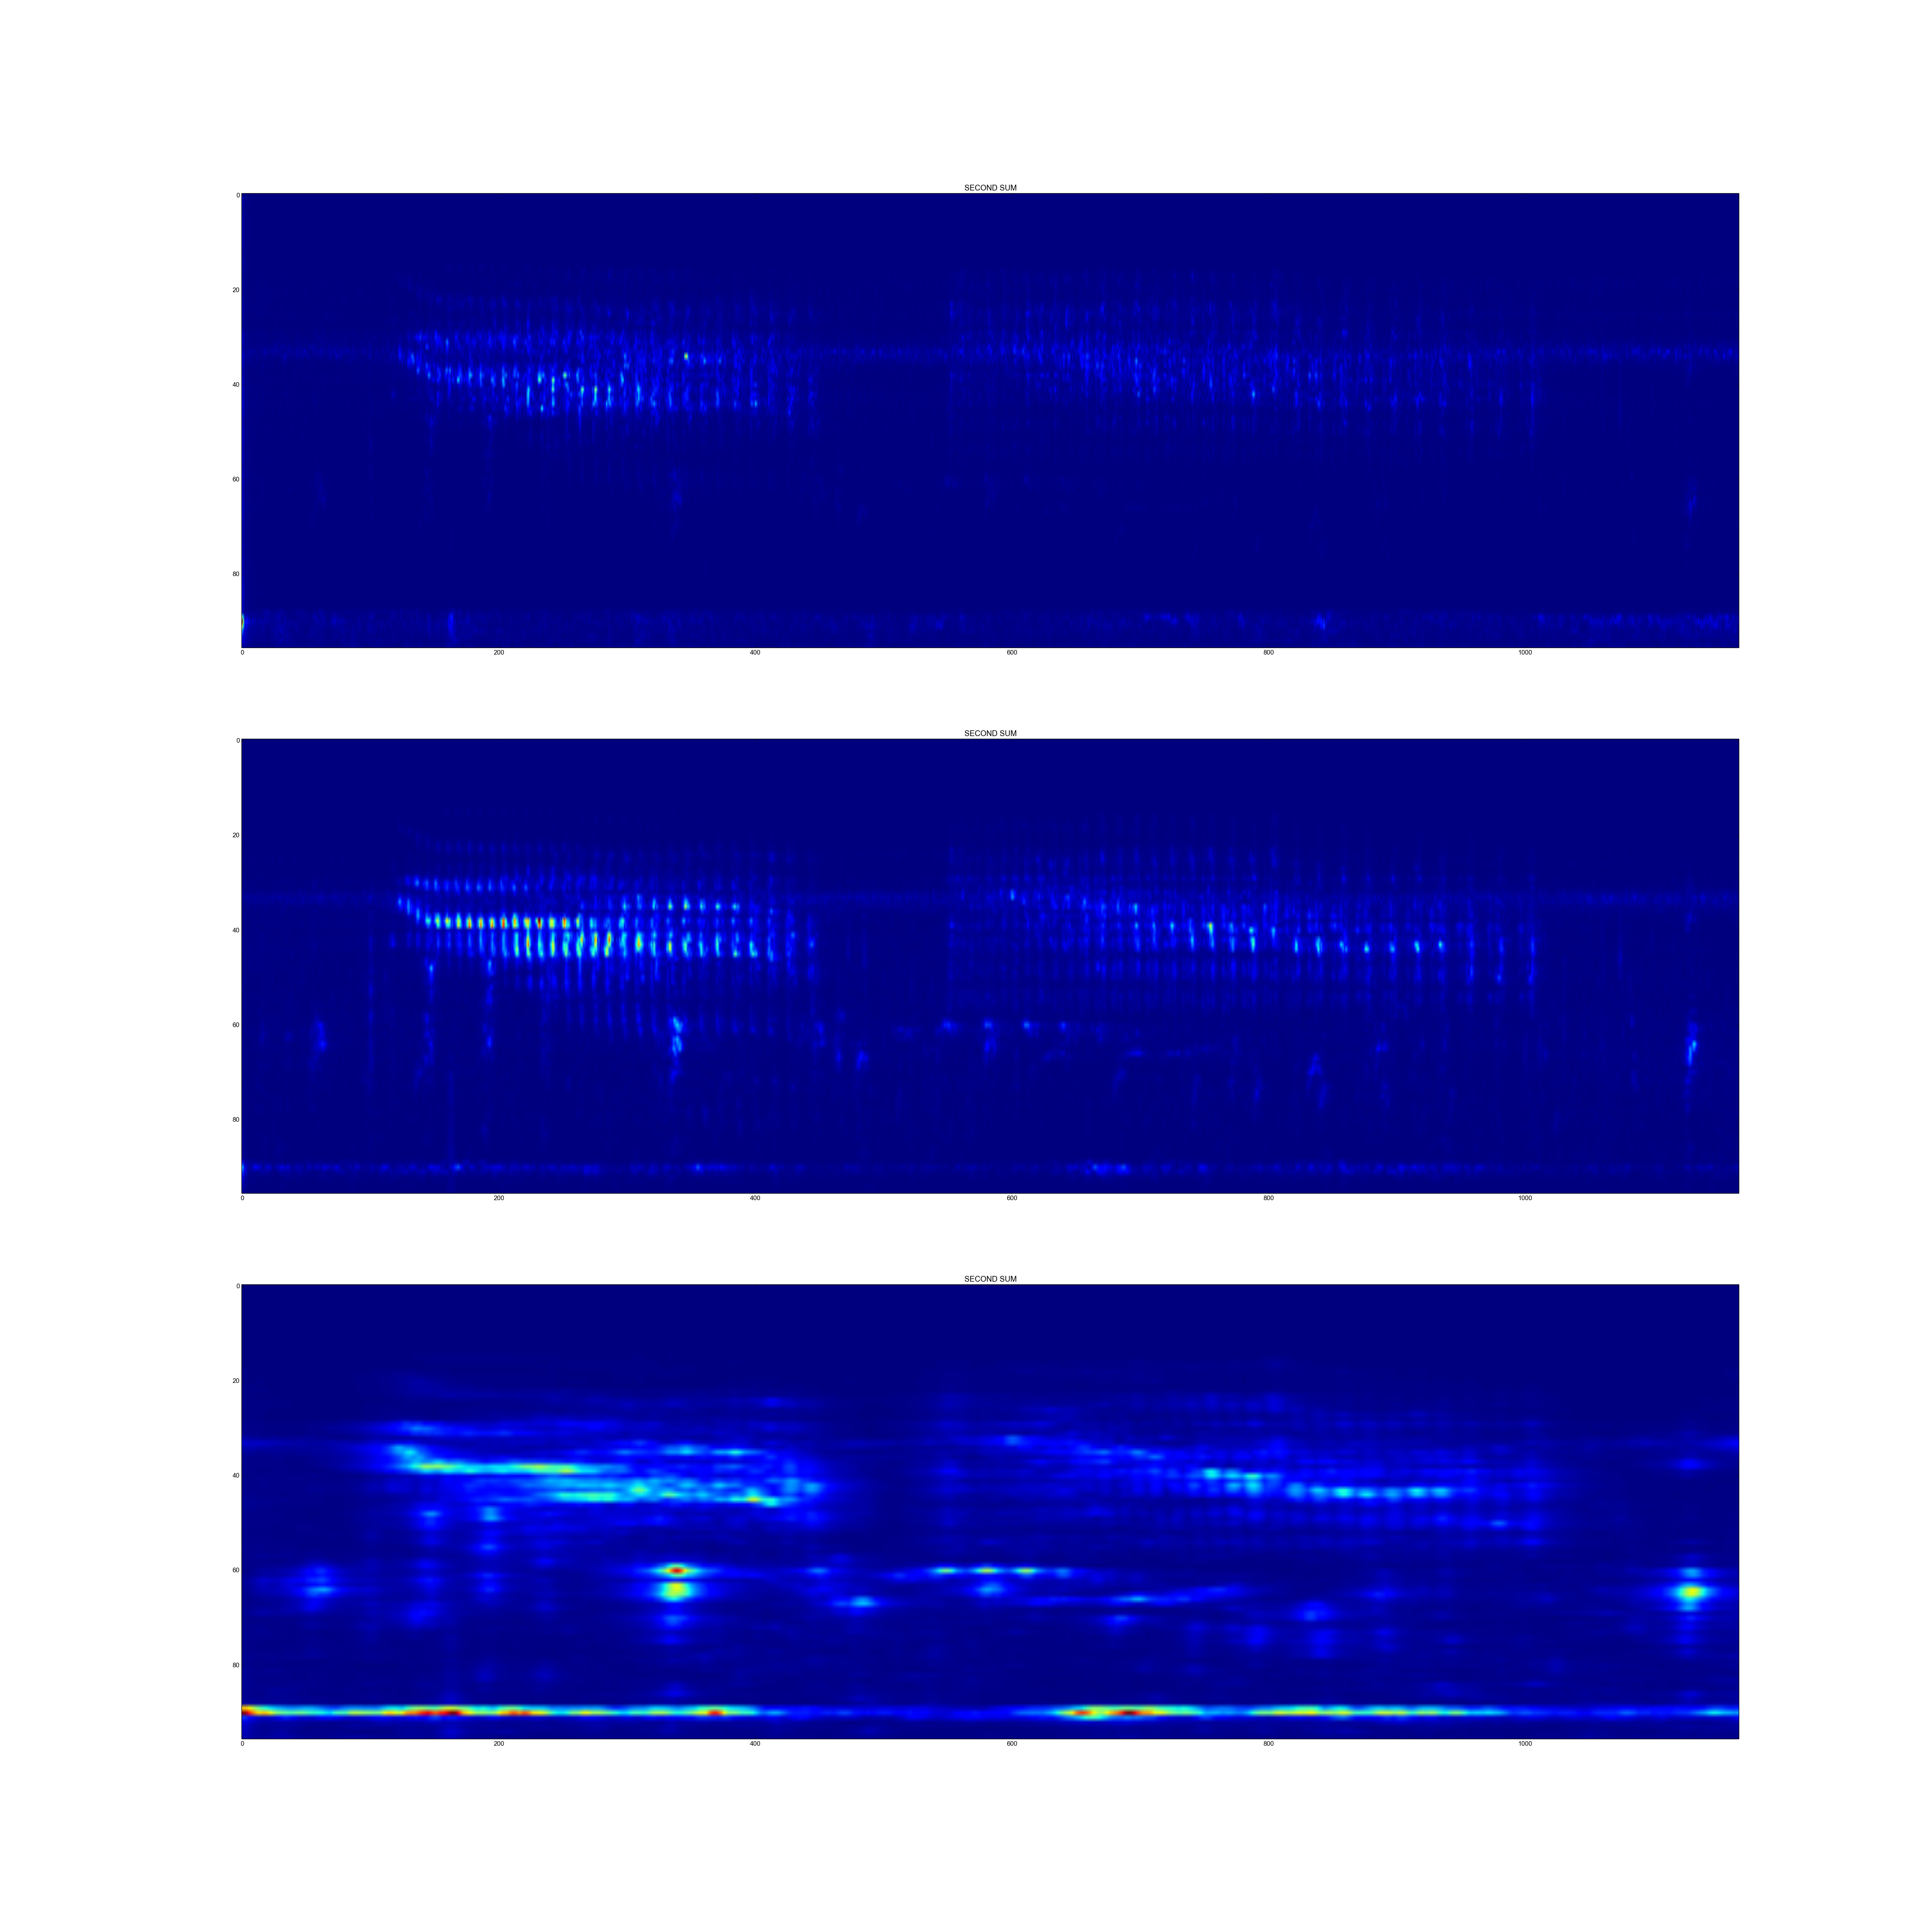
\includegraphics[scale=0.1]{RN819_3.png}\caption{Each subplot $j=0,1,2$ is equal to $\sum_{i=0}^4 U_{2,j*5+i}$ representing an element wise addition of the previous subplots ($5$ by $5$ with $\beta_i=1\forall i$ so no thresholding of a particular $\psi_{2,i}$) }
\end{center}
\end{figure}
In this last case we can see that a "denoising" technique such as explained in the automatic feature extractor could be efficient.\\
Note that before the linear combination all the layers have been normalized independently from each other so their values are between $0$ and $1$.

\subsection{Constant Weighting}
In this case we are using $\beta_i=1, \forall i$ if we are treating the normalized decompositions, otherwise we use $\beta_i=\frac{1}{max(|U_1 \star \psi_{2,i}|\star \phi_2)}$ in order to have a "normalized version" of the decompositions. The thing here is not to threshold but to aggregate the information in order to reduce the feature vector length. it is import to note that the features computed (mean,max,std) are sensitive to this change. \\
Once again, we need to cross-validate the $T_2$ coefficient.
\begin{figure}[H]
\begin{center}
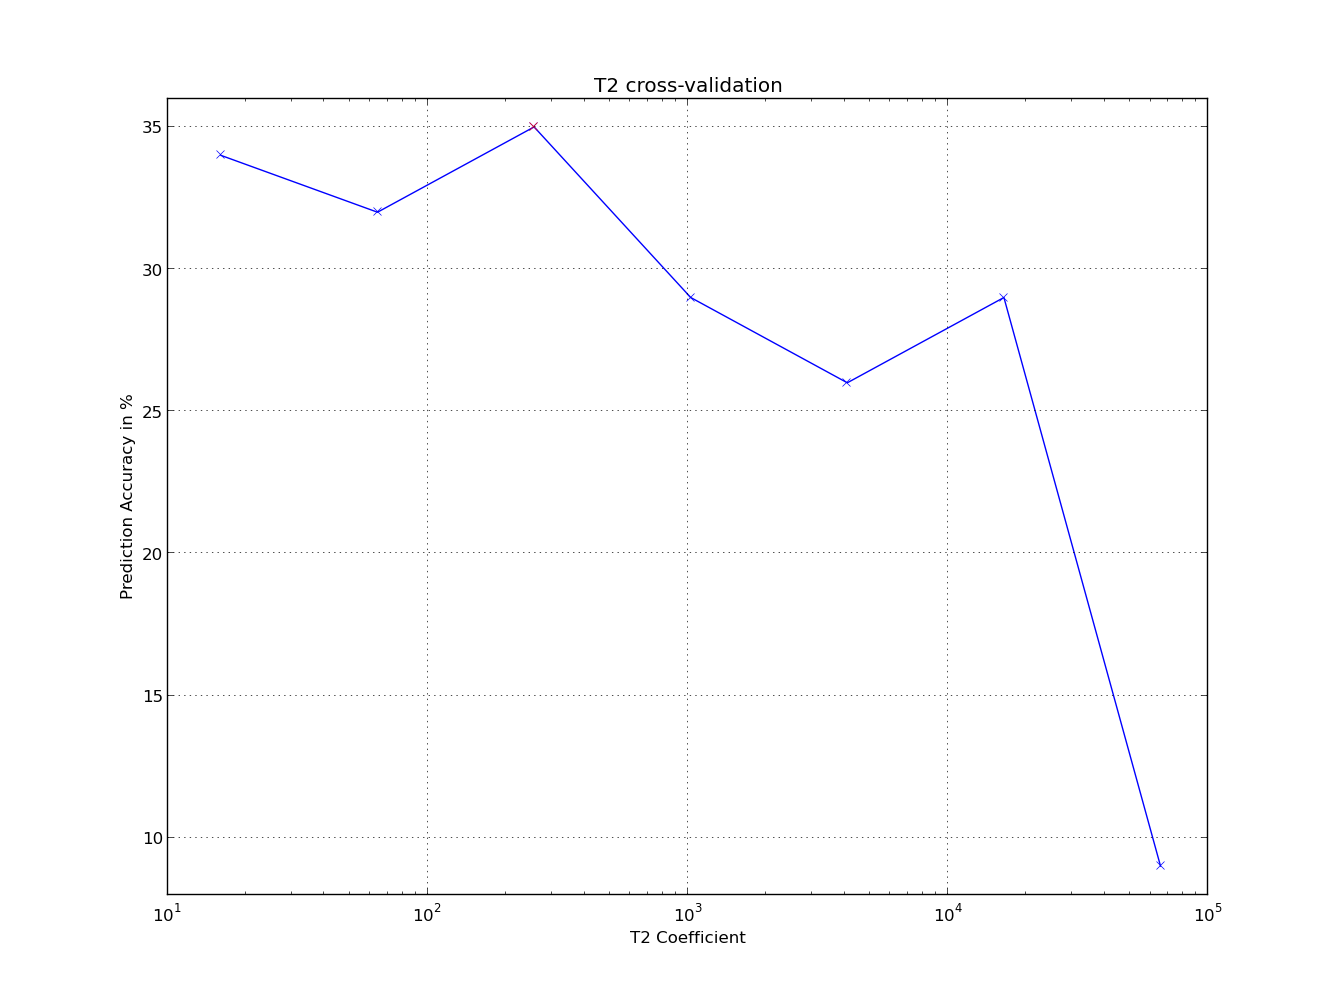
\includegraphics[scale=0.3]{cross_T2_agregated.png}\caption{Cross-validation on $T_2$ using std, mean and max features of the aggregated $S_2'$ ($80*3$ coefficients) without thresholding a particular $\psi_{2,\lambda_2}$}
\end{center}
\end{figure}
The features are also optimized :
\begin{figure}[H]
\begin{center}
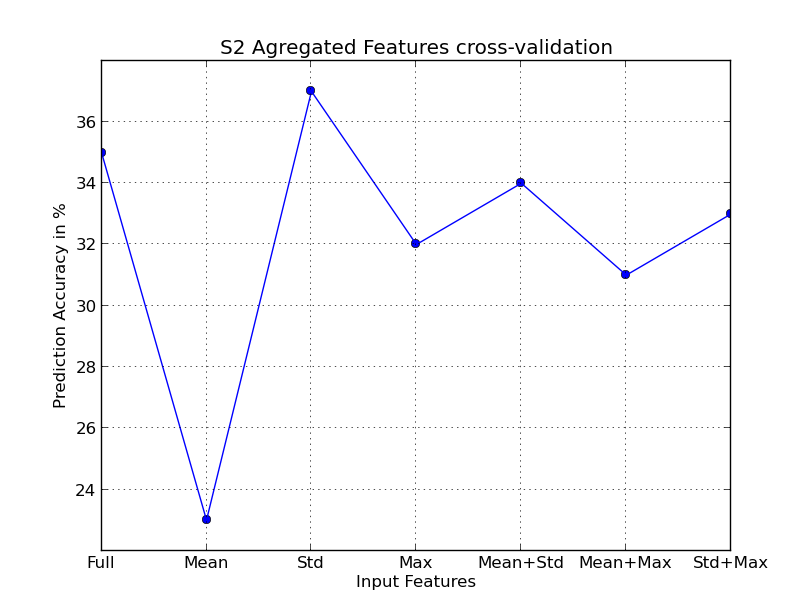
\includegraphics[scale=0.5]{cross_features_S0_S1_agregated.png}\caption{Cross-validation on the features}
\end{center}
\end{figure}
Now that our representation has been optimized we can cross-validate the number of hidden-neurons in our classifier.

\begin{figure}[H]
\begin{center}
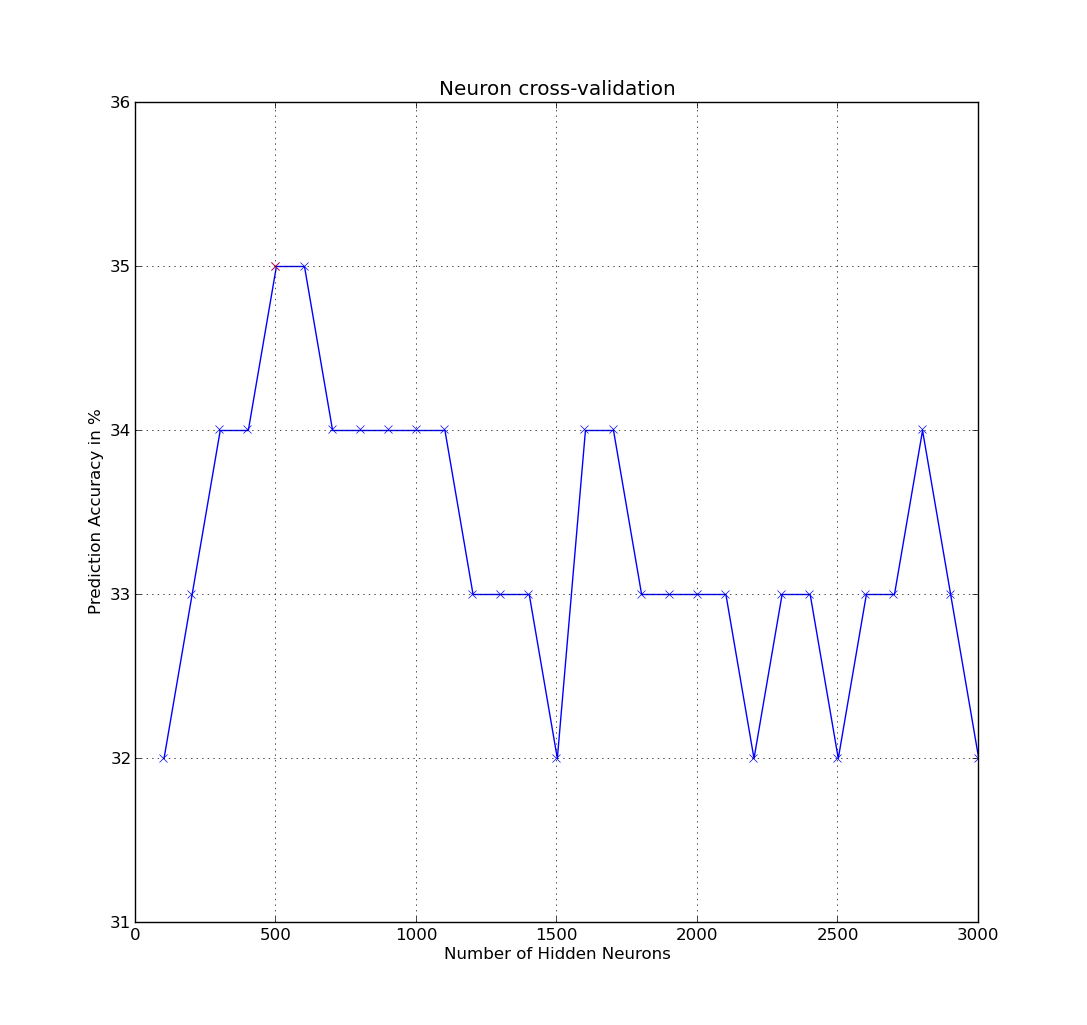
\includegraphics[scale=0.3]{cross_neuron_S2_agreg.png}\caption{Cross-validation on the number of hidden neurons}
\end{center}
\end{figure}
We can then reach an accuracy of $35\%$ by simply aggregating information. Even though the improvement is not huge (only $2\%$) we will now see that introducing active weighting can drastically improve this result.
\subsection{Pyramidal Weighting}
The coefficients $\beta_i$ are now of the form 

\begin{figure}[H]
\begin{center}
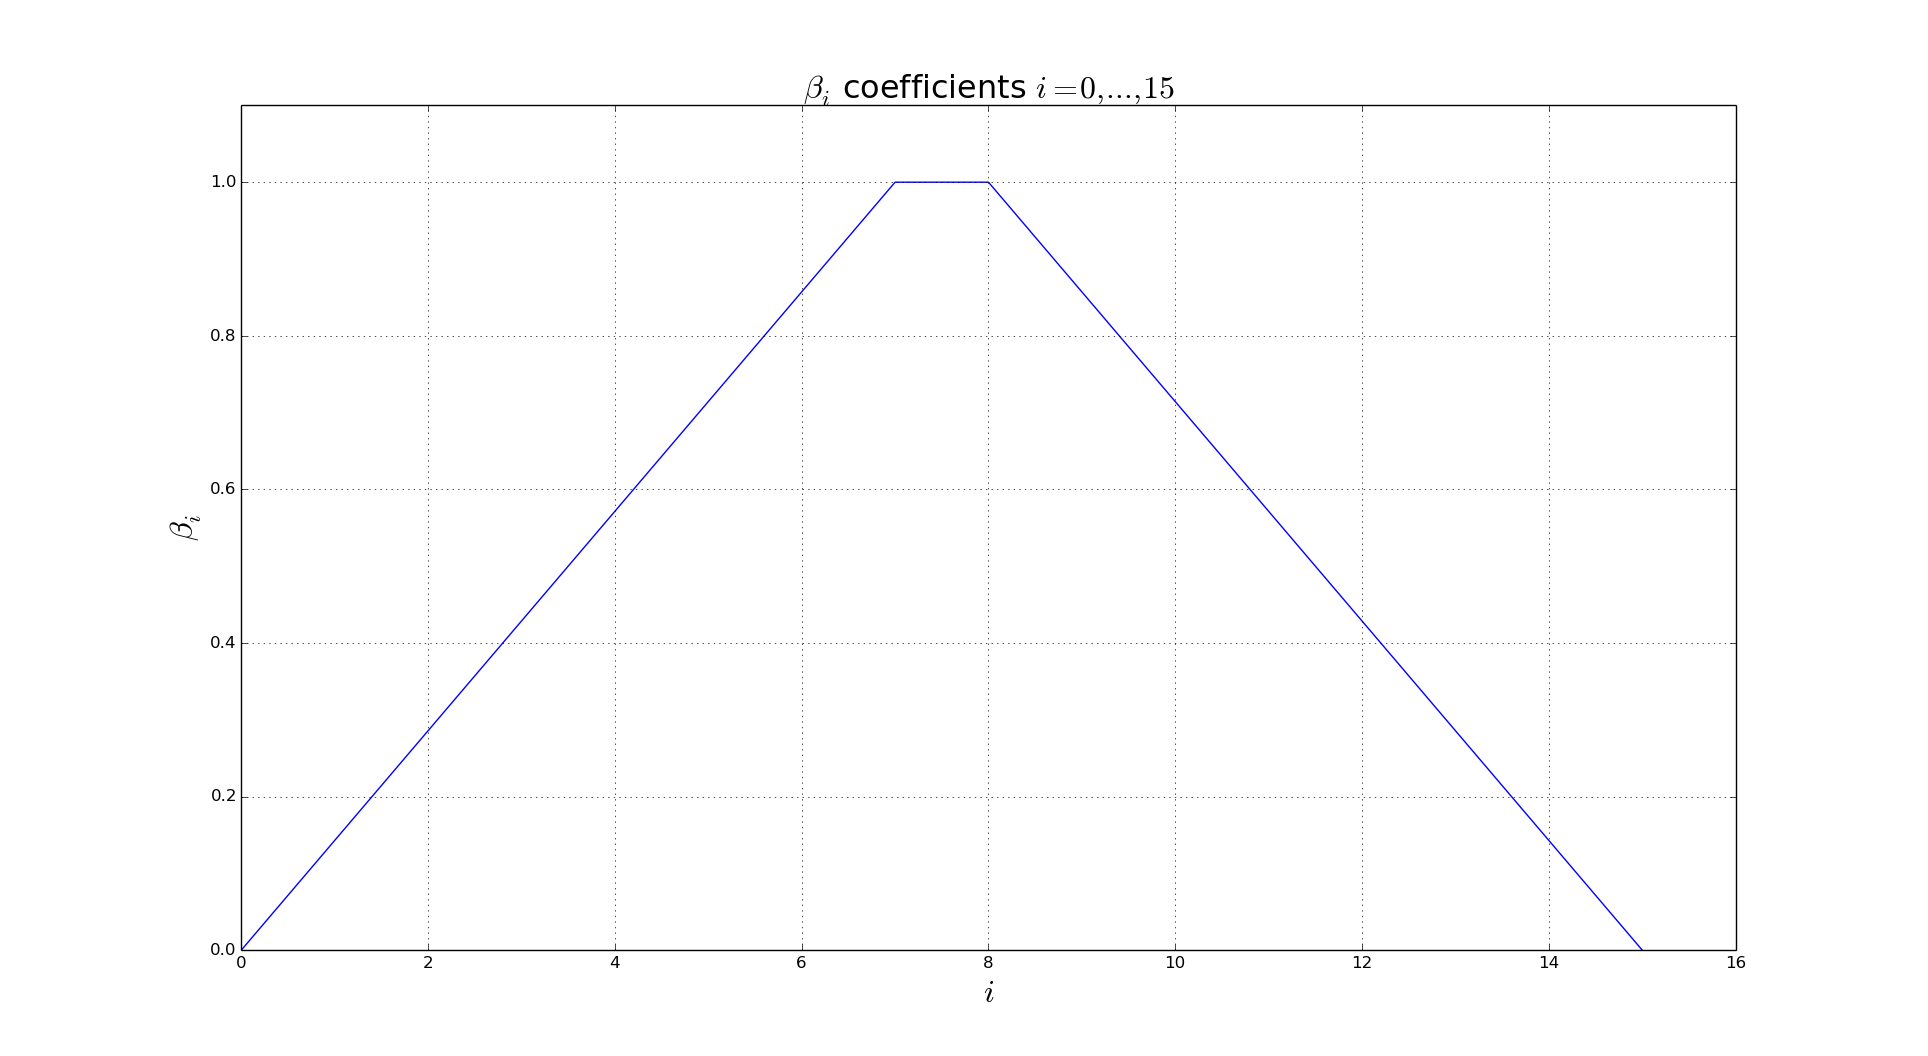
\includegraphics[scale=0.2]{b_i_coeffs.png}\caption{The chosen coefficients for the thresholding}
\end{center}
\end{figure}
and then the coefficients are weighted by the normalization so : $\beta_i*=\frac{1}{max(|U_1 \star \psi_{2,i}|\star \phi_2)}$
thus, we hardly threshold the extreme cases. This is from the fact that insects are usually present for the first filters and background noises are encoded by the last filters.
\\
Let's now cross-validate the $T_2$ coefficient :
\begin{figure}[H]
\begin{center}
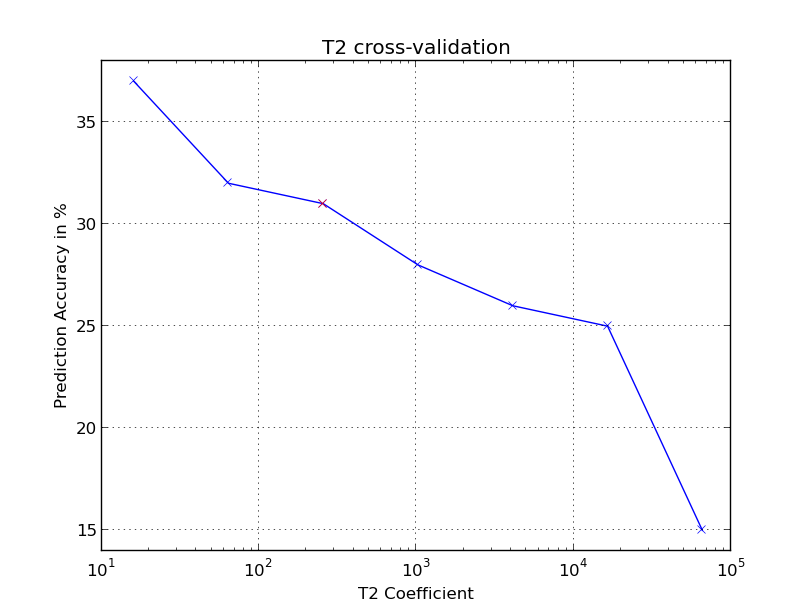
\includegraphics[scale=0.5]{cross_T2_weighted_agregated.png}\caption{Cross-validation on the $T_2$ for pyramidal coefficients}
\end{center}
\end{figure}
And now we cross-validate the features :
\begin{figure}[H]
\begin{center}
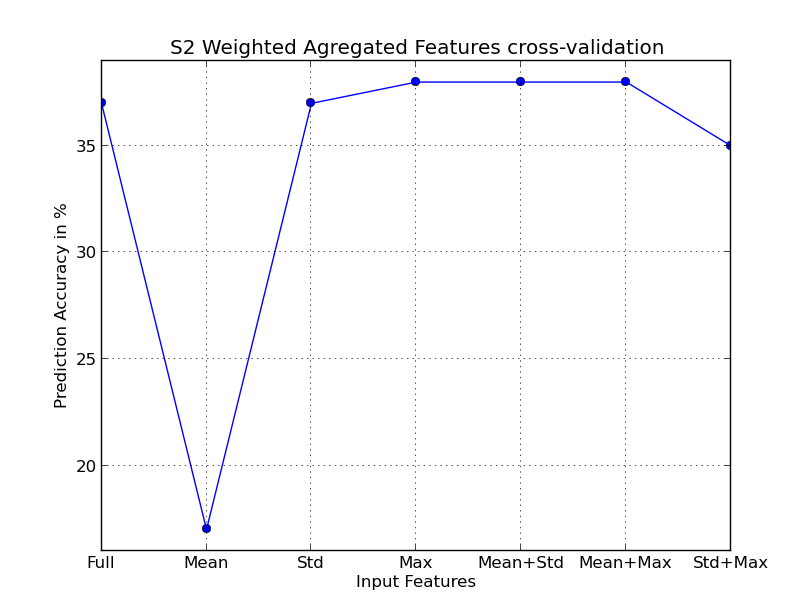
\includegraphics[scale=0.5]{cross_features_S0_S1_weighted.png}\caption{Cross-validation on the $S_2'$ features for pyramidal coefficients}
\end{center}
\end{figure}
We finally cross-validate the classifier and see the impact on the accuracy :
\begin{figure}[H]
\begin{center}
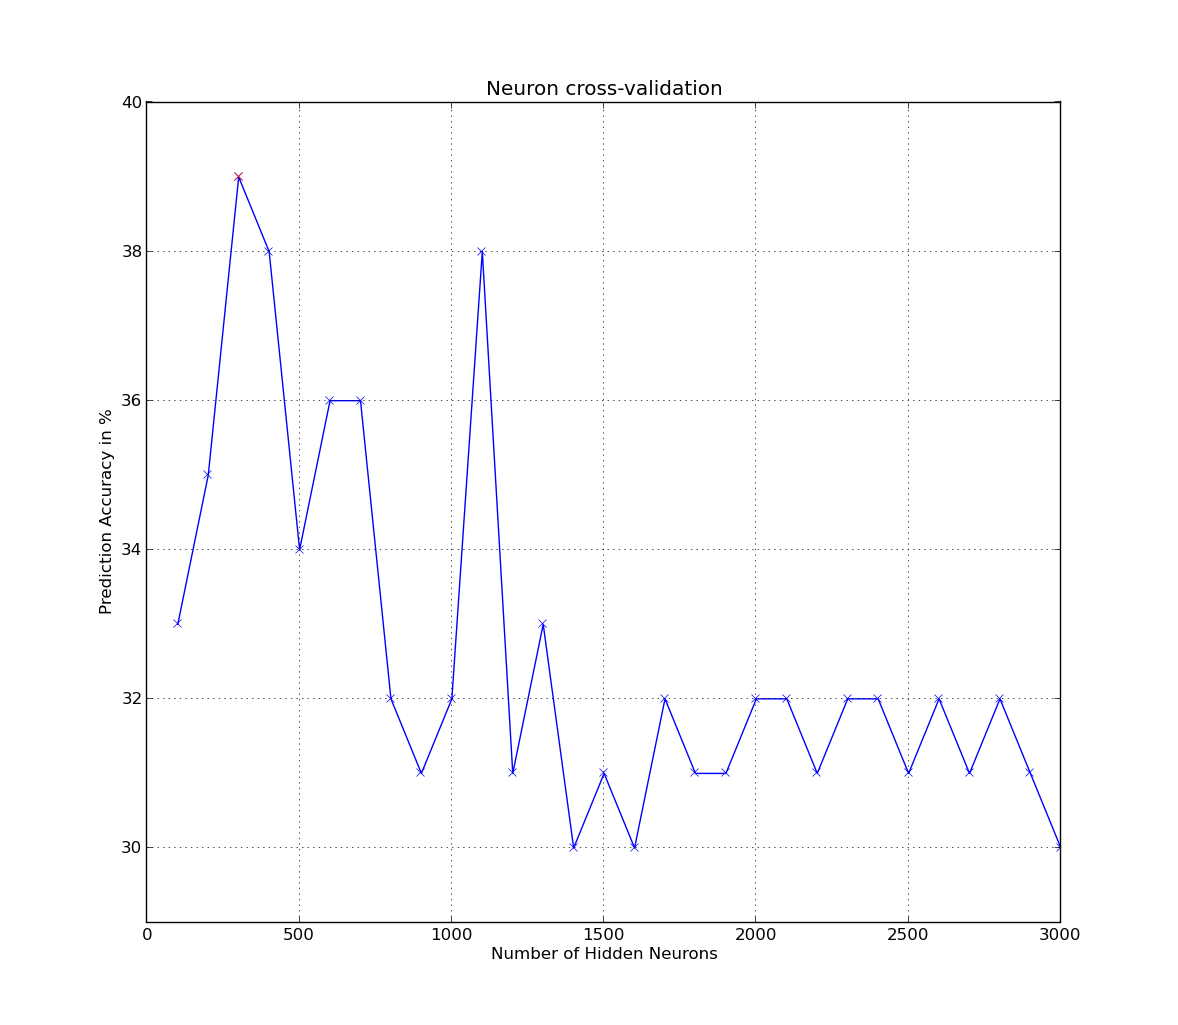
\includegraphics[scale=0.3]{cross_neuron_S2_weighted.png}\caption{Cross-validation on the number of hidden neurons}
\end{center}
\end{figure}
It is now clear that the weighting is playing an important role for the accuracy. We are able to reach $39\%$ of accuracy with this coefficients and architecture which is yet another improvement from constant coefficients.
\subsection{Results Summary and Discussions}
Clearly with this approach we are able to have an information gain while keeping a low dimension.
The main drawback concerns the selection of the thresholding coefficients $\beta_i$ and the second layer coefficients $Q_2$, $J_2$.
For example, another trial with $Q_2=1,J_2=14$ leads to $54\%$ of accuracy using $\beta_i=1,\forall i$. This approach is clearly the one to investigate. Choosing a small $Q_2$ seems enough since more filters per octave would lead to redundant layers ($|U_1 \star \psi_{2,i}| \approx |U_1 \star \psi_{2,i \pm 1 }|$). On the other hand, having a bigger $J_2$ is better since it allows more  information gain in the middle to low frequencies (usually where birds are). 
\chapter{Discussion and Conclusion}
\section{Discussion}
\subsection{Three Layers with $U_2$ Thresholding}
The goal here is to use the thresholding algorithm of the $\psi_{2,\lambda_2}$ in order to then make another scattering layer decomposing the $U_2'$ which would be "cleaner" than a standard $U_2$. This would provide more information on the bird songs while keeping a thresholding phase and dimensionality reduction part. The scheme would be as follow for the last part :
\begin{align*}
... \rightarrow & | U'_2 \star \psi_{3,\lambda_3}| :=U_3'(\lambda_1,k(\lambda_2),\lambda_3,t)\\
& \downarrow\\
& U'_3 \star \phi_3 := S'_3(\lambda_1, k(\lambda_2),\lambda_3,t) \in \mathbb{R}^{| \lambda_1 | * | \lambda_3| \times N_3}
\end{align*}
\subsection{Image Classification}
Another way could be to first use compute a scalogram or spectrogram (a time-frequency representation) and then treat this as an image. This task would then be to classify textures for example. It could even be possible to perform some kind of edge detections to first extract the $2D$ features and then apply a simple classifier. 
\subsection{Speech Recognition : HMM}
Finally, an approach using a Hidden Markov Model could be used similarly to the speech recognition task. In fact, some bird songs have been artificially generated through this kind of model. 
\section{Conclusion}


The presented challenge is really a unique experience for testing algorithms around bioacoustic classification. This task contains all the main difficulties and problems encountered in a real life problem while involving a huge dataset. 
\\
We have seen that the scattering transform provides a wonderful new data representation but it is not yet easy to know how to extract features from its coefficients. We obviously didn't try every possible algorithm but the idea of thresholding/combination in the $\lambda_2$ dimension seems to be interesting. The key part is to be able to capture feature with a time-invariant algorithm in term of the position of the feature in a signal, but, we need to keep a "time" component to analyse frequencies evolution inside the features.
\\

Given the massive dataset it has also been a unique experience to learn ways and methods to deal with computational limitations and the challenge deadline.
more importantly, this has helped to deeply understand the scattering network and the pre-processing part in general when trying to apply machine learning algorithms for a given task.


\chapter*{Acknowledgements}
I particularly want to thank Pr St\'ephane MALLAT for accepting me into his team for months during this TER and for guiding me through this task. I also want to thank all his team and especially Vincent LOSTANLEN with whom I learned a lot about machine learning in general and the right way to approach such a problem. 
I thank Pr. Herv\'e GLOTIN and his team who  allowed me to use their server and for all their advices and analysis on bioacoustic and signal processing in general.
I also thank the SABIOD Project \footnote{\url{http://sabiod.org}}
MI CNRS MASTODONS for supporting me.
Finally, I want to thank Pr Albert COHEN for tutoring this TER and Pierre et Marie Curie University for giving us such opportunities.

\bibliographystyle{plain}
\bibliography{ref2}
\nocite{*}

\end{document}
